% Most users will need to modify ONLY the parts in this file that are marked as ``MODIFY ME''
%%%%%%%%%%%%%%%
%%%%%%%%%%%%%%%
% SHSU STYLE
%%%%%%%%%%%%%%%
%%%%%%%%%%%%%%%

% Set up the documentclass
\documentclass[letterpaper, oneside, onecolumn, 12pt, pdftex, titlepage]{book} 

\setcounter{secnumdepth}{0}
%%%%%%%%%%%%%%%
% NEW TIMES ROMAN
\usepackage[T1]{fontenc}
\usepackage{mathptmx}
%%%%%%%%%%%%%%%

%%%%%%%%%%%%%%%%
%TITLE PAGE
\renewcommand\maketitle{
\null  % Empty line
\nointerlineskip  % No skip for prev line
%\vfill
\begin{center}
    \normalsize
    \MakeUppercase{\thesisname}
    \vspace{1cm}\\
    \rule{6em}{0.4pt}\\
    \vspace{0.5cm}
    {\normalsize
    A Thesis\\
    Presented to\\
    The Faculty of the Department of Biological Sciences\\
    at \university\\
\vspace{0.5cm}    
    \rule{6em}{0.4pt}\\
    \vspace{0.5cm}
    In Partial Fulfillment\\
    of the Requirements for the Degree of\\
    \degreename\\
    \vspace{0.5cm}
    \rule{6em}{0.4pt}\\
    \vspace{0.5cm}
    by\\
    \authorname\\
}
    \monthyear
\end{center}
\vfill
\thispagestyle{empty}
}
%%%%%%%%%%%%%%%
% PAGE MARGINS
%
% INSTRUCTIONS: 
% The default page margins might not give the desired result 
% this depends on the type of machine that you use to compile and print
% If neither of the three choices below provide the correct margins the library demands
% CREATE A NEW geometry and set the values that work for you.
%
% These margins work on a Mac computer with MacTex and printed from a Mac computer
\usepackage[letterpaper, scale=1, nomarginpar, left=1.5truein, right=1truein, top=1truein, bottom=1truein, headheight=0.5truein, footskip=0.5truein]{geometry}
%
% DO NOT USE THE FOLLOWING MARGINS UNLESS YOU HAVE TRIPLE CHECKED THAT THE ABOVE DEFAULTS DO NOT WORK FOR YOU
%
% These margins worked on a Mac computer compiled with MacTex and the 
% printed from a Windows computer
%\usepackage[letterpaper, scale=1, nomarginpar, left=1.375truein, right=0.875truein, top=0.875truein, bottom=0.875truein, headheight=0.5truein, headsep=0.4166truein, footskip=0.5625truein]{geometry}
%
% These margins worked on a Windows computer compiling with MiKTeX
%\usepackage[letterpaper, scale=1, nomarginpar, left=1.5truein, right=0.98truein, top=1truein, bottom=0.88truein, headheight=0.5truein, headsep=0.3truein, footskip=0.333truein]{geometry}
%%%%%%%%%%%%%%%

%%%%%%%%%%%%%%%
% DOUBLE SPACING
% 
% INSTRUCTIONS: 
% The command \doublespacing may not work for you, 
% since Word double spacing is different than 
% LaTeX double spacing.
% If the library is not happy with the results of this command
% comment \doublespacing and uncomment \setstretch. 
% Then play with the number there until you get the double-spacing that is required
%The default value of 1.91666 has worked in the past
\usepackage{setspace}
%\doublespacing
\setstretch{1.91666}
% Extra vertical space inserted before a paragraph.
\setlength{\parskip}{0pt}
% Prevents LaTeX from adding vertical white space 
% in strange places on pages that it cannot fill properly.
\raggedbottom
%%%%%%%%%%%%%%%

%%%%%%%%%%%%%%%
%GENERAL STYLE
%%%%%%%%%%%%%%%
%
%%%%%%%%%%%%%%%
% These commands will help LaTeX 
% minimize the number of orphans and widows.
\doublehyphendemerits=10000       % No consecutive line hyphens.
\brokenpenalty=10000              % No broken words across columns/pages.
\widowpenalty=9999                % Almost no widows at bottom of page.
\clubpenalty=9999                 % Almost no orphans at top of page.
\interfootnotelinepenalty=9999    % Almost never break footnotes.
%%%%%%%%%%%%%%%
%
%%%%%%%%%%%%%%%
% Alter some LaTeX defaults for better treatment of figures:
% See p.105 of "TeX Unbound" for suggested values.
% See pp. 199-200 of Lamport's "LaTeX" book for details.
\renewcommand{\topfraction}{0.9}	% max fraction of floats at top
\renewcommand{\bottomfraction}{0.8}	% max fraction of floats at bottom
% Parameters for TEXT pages (not float pages):
\setcounter{topnumber}{2}
\setcounter{bottomnumber}{2}
\setcounter{totalnumber}{4}     % 2 may work better
\setcounter{dbltopnumber}{2}    % for 2-column pages
\renewcommand{\dbltopfraction}{0.9}	% fit big float above 2-col. text
\renewcommand{\textfraction}{0.1}	% allow minimal text w. figs .07 may work better
%   Parameters for FLOAT pages (not text pages):
\renewcommand{\floatpagefraction}{0.7}	% require fuller float pages
% N.B.: floatpagefraction MUST be less than topfraction !!
\renewcommand{\dblfloatpagefraction}{0.7}	% require fuller float pages
% remember to use [htp] or [htpb] for placement

%ROMAN NUMERAL CHAPTER NUMBERS
\renewcommand{\thechapter}{\Roman{chapter}}
%Bold tables
%\renewcommand{\tablename}{\textbf{Table}}
%%%%%%%%%%%%%%%

%%%%%%%%%%%%%%%
% PACKAGES
%
% The usual AMS stuff
\usepackage{amsmath,amsfonts,amssymb,amscd,amsthm}
%
%provides extensions to amsmath
\usepackage{mathtools}
%

% This package modifies the captions. 
% Only needed if the library requests to modify the captions.
% In this case, copy/paste the following line and modify the default values
% to achieve the desired result. 
%\usepackage[format=hang,labelfont=bf,font=normal,justification=centerlast, margin=20pt]{caption,subfig}
%
% This package is required to include external figures in your document.
\usepackage{graphicx}
%
% enables you to do nice figures in LATEX.
\usepackage{tikz}
%tkz-graph loads tikz but it is not contained in the standard distribution.
% \usepackage{tkz-graph}
\usetikzlibrary{matrix,arrows,shapes}
%
% This package allows a line break of an underline sentence
\usepackage{soul}
%
% If an eps image is detected, epstopdf is automatically called to convert it to pdf format.
\usepackage{epstopdf}
%
% INSTRUCTIONS:
% If you need to use a package that is not included already,
% you must add it to the file packages.tex
%%%%%%%%%%
%%%%%%%%%%
% PACKAGES
%%%%%%%%%%
%%%%%%%%%%

%%%%%%%%%%%%%%%%%%%%%%%%%%%%%%%%%%%%%%%
% I have added the packages I need to provide the correct formatting. 
% I have also added some packages that are commonly used.
% If you need to add more packages then you should do it at the end of this list.
%%%%%%%%%%%%%%%%%%%%%%%%%%%%%%%%%%%%%%%
%
% This package defines commands to access bold math symbols.  through \bm
%\usepackage{bm} 


%
% This package provide some additional commands to enhance
% the quality of tables in LaTeX.
\usepackage{booktabs}
%
% This package defines a single environment tabu to make all kinds of tabulars in text or in math mode provided that they do not split across pages.
% tabu is more flexible that tabular, tabular*, tabularx and array and extends the possibilities.
\usepackage{tabu}
%
% delarray introduces delimeters \begin{array}({cc})
% The tabulary environment expands specific columns to meet the table’s width requirement 
\usepackage{array,delarray,tabulary,colortbl}
%
% enumitem package permits adjustment of list parameters
%\begin{enumerate}[topsep=0pt, partopsep=0pt]
%to suppress all spacing above and below your list
%\begin{enumerate}[itemsep=2pt,parsep=2pt]
%to set spacing between items and between paragraphs within items
%\begin{enumerate}[label=(\emph{\alph*})] or \Alph, \arabic, \roman and \Roman
\usepackage{enumitem} 
%
% Provides:
% the IEEE itemize, enumerate and description list environments
% the complete IEEEeqnarray family for producing multiline equations
% as well as matrices and tables, including the IEEEeqnarray support
% commands.
% This package clashes with enumitem
% \usepackage[retainorgcmds]{IEEEtrantools}
%
% Create tabular cells spanning multiple rows.
\usepackage{multirow}
%
% The package rotating gives you the possibility to rotate any object of an arbitrary angle. 
\usepackage{rotating}
%
% Provides command adjustwidth to locally change the margins of the text, and commands \changetext and \changepage for more radical changes to the page design mid-way through a document.
\usepackage{changepage}
%
% This package provides a verbatim command which is useful in case you want to 
% include the outcome of a computation exactly like it is displayed on the computer.
\usepackage{verbatim}
%
% float provides the option [H] for floating environments
% \afterpage, that causes the commands specified in its argument to be expanded
% after the curent page is output 
% afterpage places the float 'somewhere close' 
% \afterpage{\clearpage\begin{figure}[H] ...\end{figure}}
%\usepackage{afterpage,float}
%
% Using the package listings you can add non-formatted text as you would do with \begin{verbatim} but its main aim is to include the source code of any programming language within your document. 
%\usepackage{listings}
%
% \xspace should be used at the end of a macro designed to be used mainly in text. 
% It adds a space unless the macro is followed by certain punctuation characters.
%\usepackage{xspace}
%
%to anable \mathscr command for math script fonts
\usepackage[mathscr]{euscript}
%
% The mathrsfs package uses a really fancy script font (the name stands for "Ralph Smith's Formal Script") which is already part of most modern TeX distributions. 
% The package creates a new command \mathscr.
%\usepackage{mathrsfs}
%
% Martin Vogel's Symbols (marvosym) font.
% \usepackage{marvosym}
%
% Fonts and macros for IPA phonetics characters.
%\usepackage{tipa}
\usepackage{makecell}
%\usepackage{enumitem}

\usepackage{lscape}
\usepackage[section]{placeins}

%Nice SI units
\usepackage{siunitx}


\endinput

%-----------------------------------------------------------------------
% End of packages.tex
%-----------------------------------------------------------------------

%%%%%%%%%%%%%%%

%%%%%%%%%%%%%%%
% This package changes the way footnotes are presented.
%\usepackage[perpage,para,symbol,bottom]{footmisc}
\usepackage[perpage,bottom,flushmargin]{footmisc}
%%%%%%%%%%%%%%%

%%%%%%%%%%%%%%%
% PAGE FORMATTING
% This package makes every page number to appear
% in the top right corner.
\usepackage{fancyhdr}
\pagestyle{fancy}
\fancyhf{} 
\rhead{\rm\thepage}
\renewcommand\headrulewidth{0pt}
%%%%%%%%%%%%%%%

%%%%%%%%%%%%%%%
% NUMBERING OF TABLES, FIGURES, AND EQUATIONS
\usepackage{chngcntr}
\counterwithout{table}{chapter}
\counterwithout{figure}{chapter}
\counterwithout{equation}{chapter}
%%%%%%%%%%%%%%%

%%%%%%%%%%%%%%%
% TABLE OF CONTENTS
% The header may appear a bit off the top margin.
% If that is the case, use the second definition and 
% adjust the vertical space accordingly.
\renewcommand{\contentsname}{TABLE OF CONTENTS}
%\renewcommand{\contentsname}{\protect\vspace{0.09375in}TABLE OF CONTENTS}
%
% Only Chapters and Sections are needed in TOC.
\setcounter{tocdepth}{1}

% The word "Page" must appear in TOC.
% The placing of the word "Page"  in the TOC may need to be fixed.
% If so, change ~\hfill for \hspace{5.65in} or whatever quantity works for you.
\addtocontents{toc}{~\hfill\textbf{Page}\par}
%%%%%%%%%%%%%%%
%
%%%%%%%%%%%%%%%
% This package modifies the table of contents
% The TOC is indented according to depth: Chapter, Section.
% However, I decided to use titletoc instead since it provides
% more capabilities. But this command is as easy as pie. 
% You just add the package and that is it.
%\usepackage{tocstyle}
%%%%%%%%%%%%%%%
%
%%%%%%%%%%%%%%%%
% This package also modifies the table of contents
% The right margin can be controlled much more
% which is needed in order not to intrude into the 1in margin
% that is required by the library.
\usepackage{titletoc}
%
% The next line writes the dots all the way to the number 
%\contentsmargin{0pt}
%
% The next line shrinks the width of the TOC in case it is needed. 
%\renewcommand\contentspage{\thecontentspage}
%
% \dottedcontents  fills the page with dots up to the page number.
% However it makes the entries have bold font.
% So I created my own version of below.
%\dottedcontents{chapter}[2em]{}{2em}{1pc} % 2.3, 2.3, 5pt
%\dottedcontents{section}[3.8em]{}{2em}{1pc} %3.8, 2.3
%
% INSTRUCTIONS:
% Depending on the final margins of your document,
% some of the values below may need to change.
\titlecontents{chapter} % set formatting for \chapter 
[2.3em]                 % adjust left margin
{\normalfont}           % font formatting
{\contentslabel{1.3em}} % section label and offset
{\hspace*{-2.3em}} 
{\titlerule*[1pc]{.}\contentspage}
\titlecontents{section} % set formatting for \section 
[6em]                 % adjust left margin
{\normalfont}             % font formatting
{\contentslabel{2.5em}} % section label and offset
{\hspace*{-2.3em}}
{\titlerule*[1pc]{.}\contentspage}
%%%%%%%%%%%%%%%%

%%%%%%%%%%%%%%%
% TABLE OF LISTS AND FIGURES
% INSTRUCTIONS:
% The headers may appear a bit off the top margin.
% If that is the case, use the second definitions and 
% adjust the vertical space accordingly.
\renewcommand\listtablename{LIST OF TABLES}
\renewcommand\listfigurename{LIST OF FIGURES}
%\renewcommand\listtablename{\protect\vspace{0.09375in}LIST OF TABLES}
%\renewcommand\listfigurename{\protect\vspace{0.09375in} LIST OF FIGURES}
\addtocontents{lot}{\textbf{Table}\hfill\textbf{Page}\par}
\addtocontents{lof}{\textbf{Figure}\hfill\textbf{Page}\par}
% These command prevents LaTeX from adding extra space 
% in the LOF and LOT between items on different chapters.
\newcommand*{\noaddvspace}{\renewcommand*{\addvspace}[1]{}}
\addtocontents{lot}{\protect\noaddvspace}
\addtocontents{lof}{\protect\noaddvspace}
%%%%%%%%%%%%%%%
%
%%%%%%%%%%%%%%%
% Shrink the horizontal spacing in LOT and LOF
% tocloft conflicts  with titletoc
% \usepackage{tocloft}
% \addtolength{\cftfignumwidth}{-1em}
% \addtolength{\cfttabnumwidth}{-1em}
%%%%%%%%%%%%%%%

%%%%%%%%%%%%%%%
% CHAPTER AND SECTION HEADINGS
% I would like to use the line below, but it creates some issues with
% my definitions below. So I am using a vanilla version of the package.
%\usepackage[noindentafter, rigidchapters, nobottomtitles*]{titlesec}
\usepackage[nobottomtitles*]{titlesec}
% \titleformat{ command }[ shape ]{ format }{ label }{ sep }{ before }[ after ]
\titleformat{\chapter}[display]
{\normalfont\normalsize\bfseries\filcenter}
{CHAPTER \thechapter}
{0ex}
{\titlerule[0pt]
\vspace{0ex}%
}
[\vspace{0ex}%
{\titlerule[0pt]}]
%
\titleformat{\section} % add \filcenter if centering required
  {\normalfont\normalsize\bfseries}{\thesection}{1em}{}
\titleformat{\subsection} % add \filcenter if centering required
  {\normalfont\normalsize\bfseries}{\thesubsection}{1em}{} 
\titleformat{\subsubsection} % add \filcenter if centering required
  {\normalfont\normalsize\bfseries}{\thesubsubsection}{1em}{}
\titleformat{\paragraph}[runin]
  {\normalfont\normalsize\bfseries}{\theparagraph}{1em}{}
\titleformat{\subparagraph}[runin]
  {\normalfont\normalsize\bfseries}{\thesubparagraph}{1em}{}
%
% SPACING OF CHAPTER AND SECTION HEADINGS
% INSTRUCTIONS:
% The CHAPTER HEADING may be a bit low or high depending on the margins.
% If that is the case, modify the {-30pt} for whatever works.
% -28pt has also worked.
%
% The lines below gives the correct spacing in most cases.
% But it has one small inconsistency when a \chapter command
% is immediately followed by a \section command.
% In that case a line \vspace{-12pt} must be place in between
% the two commands on each occurence inside your main text.
% \titlespacing{ command }{ left }{ beforesep }{ aftersep }[ right ]
\titlespacing{\chapter} {0pt}{-30pt}{12pt}
\titlespacing{\section} {0pt}{0pt}{0pt}
\titlespacing{\subsection} {0pt}{0pt}{0pt}
\titlespacing{\subsubsection} {0pt}{0pt}{0pt}
\titlespacing{\paragraph} {0pt}{0pt}{0pt}
\titlespacing{\subparagraph} {\parindent}{0pt}{0pt}
%%%%%%%%%%%%%%%

%%%%%%%%%%%%%%%
% BIBLIOGRAPHY
% INSTRUCTIONS:
% The header may appear a bit off the top margin.
% If that is the case, use the second definition and 
% adjust the vertical space accordingly.
%\renewcommand{\bibname}{REFERENCES}
 \renewcommand{\bibname}{\protect\vspace{12pt}REFERENCES}
%
%  Bibliography prepared with BibTeX using amsplain
%  or amsalpha using natbib.
\usepackage[square, numbers, comma, sort&compress]{natbib}
% The following line deletes extra space in between the entries in the
% bibliography to keep the doublespacing.
\setlength{\bibsep}{0pt}
%%%%%%%%%%%%%%%

%%%%%%%%%%%%%%%
% APPENDIX
% This package improves some of the formatting of the title of an appendix and 
% the inclusion of the appendix in the TOC.
\usepackage{appendix}
% INSTRUCTIONS:
% The header may appear a bit off the top margin.
% If that is the case, use the second definition and 
% adjust the vertical space accordingly.
\renewcommand\appendixname{APPENDIX}
%\renewcommand\appendixname{\protect\vspace{9pt}APPENDIX}
%%%%%%%%%%%%%%%
%
%%%%%%%%%%%%%%%%%%%%%%%%%%%%%%%%
% I strongly recommend AGAINST adding the following spell.
% 
% This prepends the word APPENDIX in TOC
% for each appendix chapter.
%%%%%%%%%%%%%%%%%%%%%%%%%%%%%%%%
% \makeatletter
% \newcommand\appendix@chapter[1]{%
%  \refstepcounter{chapter}%
%  \orig@chapter*{APPENDIX \@Alph\c@chapter\ #1}%
%  \addcontentsline{toc}{chapter}{APPENDIX \@Alph\c@chapter\protect\quad #1}%
% }
% \let\orig@chapter\chapter
% \g@addto@macro\appendix{\let\chapter\appendix@chapter}
% \makeatother
%%%%%%%%%%%%%%%%%%%%%%%%%%%%%%%%%

%%%%%%%%%%%%%%%
% HYPERLINKS
\usepackage{url}
\usepackage[pdfpagemode=UseOutlines,bookmarks=true,bookmarksopen=true,
   bookmarksopenlevel=1,bookmarksnumbered=true,hypertexnames=false,
   colorlinks,linkcolor={black},citecolor={black},urlcolor={red}, unicode,
   pdfstartview=FitV,breaklinks=true]{hyperref} 

%%%%%%%%%%%%%%
%%%%%%%%%%%%%%%
%%%%%%%%%%%%%%%
% END: SHSU STYLE
%%%%%%%%%%%%%%%
%%%%%%%%%%%%%%%
\endinput


%%%%%%%%%%%%%%%%%%%
%%%%%%%%%%%%%%%%%%%
% THEOREM ENVIRONMENTS 
%%%%%%%%%%%%%%%%%%%
%%%%%%%%%%%%%%%%%%%

% As set up here, all theorem-class objects will be numbered with
% the same counter, starting with 1.
% This may be changed if the author prefers.
% For example, you can change this setup to start 
%  with 1 at every new chapter; and set numbers to have
%  the form <chapter>.<theorem>.  

%\theoremstyle{plain}
\newtheorem{theorem}{Theorem}%[chapter]
\newtheorem{lemma}[theorem]{Lemma}
\newtheorem{corollary}[theorem]{Corollary}
\newtheorem{proposition}[theorem]{Proposition}
\newtheorem{axiom}[theorem]{Axiom}
\newtheorem{algorithm}[theorem]{Algorithm}
\newtheorem{conjecture}[theorem]{Conjecture}

\theoremstyle{definition}
\newtheorem{definition}[theorem]{Definition}
\newtheorem{example}[theorem]{Example}
\newtheorem{xca}[theorem]{Exercise}

\theoremstyle{remark}
\newtheorem{remark}[theorem]{Remark}
%%%%%%%%%%%%%%%

\endinput

%-----------------------------------------------------------------------
% End of theorems.tex
%-----------------------------------------------------------------------


%%%%%%%%%%%%%%%%%%%
%%%%%%%%%%%%%%%%%%%
% LaTeX COMMANDS
%%%%%%%%%%%%%%%%%%%
%%%%%%%%%%%%%%%%%%%
%Im tired of typing grams of o2 per meter2 per day 
\sisetup{qualifier-mode = phrase, qualifier-phrase = \ } 
\DeclareSIUnit\goxy{\gram\of{O_2~}\per\square\meter\per\day}

% Miscellaneous Special Capitals
\newcommand{\zz}{\mathbb{Z}}
\newcommand{\nn}{\mathbb{N}}
\newcommand{\pp}{\mathbb{P}}
\newcommand{\qq}{\mathbb{Q}}
\newcommand{\rr}{\mathbb{R}}
\newcommand{\cc}{\mathbb{C}}
\newcommand{\kk}{\bm{k}}
\newcommand{\xx}{\bm{x}}
\newcommand{\bfa}{\bm{a}}
\newcommand{\bfb}{\bm{b}}
\newcommand{\sm}{\mathscr{M}}
\newcommand{\sg}{\mathscr{S}}
\newcommand{\LL}{\mathscr{L}}
\newcommand{\rD}{\widetilde{\Delta}}
\newcommand{\rL}{\widetilde{\LL}}
\newcommand{\rV}{\widetilde{V}}
\newcommand{\GG}{\bm{G}}
\newcommand{\HH}{\bm{H}}
\newcommand{\bfs}{\bm{s}}

%Miscellaneous symbols
\newcommand{\di}{\"}
\newcommand{\la}{\langle}
\newcommand{\ra}{\rangle}
\newcommand{\os}{\overset}
\newcommand{\us}{\underset}
\newcommand{\perpp}{\mbox{$\perp\!\!\!\perp$}}
\newcommand{\Times}{\!\times\!}
\newcommand{\lra}{\longrightarrow} 
\newcommand{\Lra}{\Longrightarrow}
\newcommand{\lto}{\longleftarrow}
\newcommand{\lf}{\left}
\newcommand{\rt}{\right}
\newcommand{\bv}{\, \big\vert \,}
\newcommand{\wt}{\widetilde}
\providecommand{\abs}[1]{\lvert#1\rvert}
\providecommand{\norm}[1]{\lVert#1\rVert}

%Miscellaneous Greek letters
\newcommand{\eps}{\ensuremath{\epsilon}}
\newcommand{\ga}{\ensuremath{\gamma}}

%Miscellaneous operators
\DeclareMathOperator{\coker}{Coker}
\DeclareMathOperator{\im}{Im}
\DeclareMathOperator{\codim}{codim}
\DeclareMathOperator{\smax}{\sigma_{\mathrm{max}}}
\DeclareMathOperator{\tail}{tail}
\DeclareMathOperator{\head}{head}
\DeclareMathOperator{\outdeg}{outdeg}
\DeclareMathOperator{\indeg}{indeg}
\DeclareMathOperator{\supp}{supp}

% Displaystyle in $$ mode
\newcommand{\ds}{\displaystyle}

%%%%%%%%%%%%%%%%%%%%%%%%%%%%%%%%%%%
% EXTRA COMMANDS 
%%%%%%%%%%%%%%%%%%%%%%%%%%%%%%%%%%%

\newcommand{\sxy}[2]{\sum_{i=#1}^{#2}}
\newcommand{\res}[3]{$ 0 \leftarrow S^{#1} \leftarrow S^{#2} \leftarrow S^{#3} \leftarrow 0$}
%  Blank box placeholder for figures 
% To reserve space that later will be used for a table or figure.
\newcommand{\blankbox}[2]{%
  \parbox{\columnwidth}{\centering
%    Set fboxsep to 0 so that the actual size of the box will match the
%    given measurements more closely.
    \setlength{\fboxsep}{0pt}%
    \fbox{\raisebox{0pt}[#2]{\hspace{#1}}}%
  }%
}
%%%%%%%%%%%%%%%%%%%%%%%%%%
%%%%%%%%%%%%%%%%%%%%%%%%%%

\endinput

%-----------------------------------------------------------------------
% End of commands.tex
%-----------------------------------------------------------------------


% \makeatletter
%  \renewcommand*\l@chapter[2]{%
%  \ifnum \c@tocdepth >\m@ne
%  \addpenalty{-\@highpenalty}%
%  \vskip \@plus\p@
%  \setlength\@tempdima{1.5em}%
%  \begingroup
%   \let\oldnumberline=\numberline
%   \def\numberline{\chaptername~\oldnumberline}%
%   \settowidth{\@tempdimb}{\normalsize\textbf \chaptername~}%
%   \advance\leftskip by \@tempdimb
%   \parindent \z@ \rightskip \@pnumwidth
%   \parfillskip -\@tempdima
%   \leavevmode \textbf
%   \advance\leftskip\@tempdima
%   \hskip -\leftskip
%   #1\nobreak\normalfont\leaders\hbox{$\m@th
%         \mkern \@dotsep mu\hbox{.}\mkern \@dotsep
%         mu$}\hfill\nobreak\hb@xt@\@pnumwidth{\hss #2}\par
%       \penalty\@highpenalty
%     \endgroup
%   \fi}

%%%%%%%%%%%%%%
%% MODIFY ME %%%%%
%%%% BEGIN %%%%%%
%%%%%%%%%%%%%%
% The following command specifies which chapters and appendices
% are included in the document.
%
% If you remove an entry from this list, the final pdf file will not include that chapter.
% But the chapter numbering, page numbering, table of contents, and other automatic counters
% will still take into account all the chapters that appear below as \include{}
%
% Note that there are no spaces in between entries in this list.
\includeonly{chap1,chap2,chap3,chap4,appendix1,vita}
%%%%%%%%%%%%%%
%%%%% END  %%%%%
%%%%%%%%%%%%%%

% \makeindex
\begin{document}
\frontmatter

%%%%%%%%%%%%%%
%% MODIFY ME %%%%%
%%%% BEGIN %%%%%%
%%%%%%%%%%%%%%
\newcommand{\thesisname}{Ecosystem  metabolism  of  coastal  Texas  streams  across  precipitation regimes and land use gradients}
\newcommand{\authorname}{Connor L. Brown}
\newcommand{\degreename}{Master of Science}
\newcommand{\fulldegreename}{Master of Science in Biology}
\newcommand{\university}{Sam Houston State University}
\newcommand{\monthyear}{May, 2022}

\maketitle
\clearpage
%%%%%%%%%%%%%
%%%%% END  %%%%%%
%%%%%%%%%%%%%%

%%%%%%%%%%%%%%%%%%%%%%%%%%%%%%%%%%%%
% You can LaTeX the Approval Sheet. However, it may
% not entirely fit the spacing of the Word template
% provided by the library.
% I AM EXTREMELY INTERESTED IN TESTING IF THIS WORKS
% To do this, uncomment the following two lines and then comment
% the third line below.
%%%%%%%%%%%%%%%%%%%%%%%%%%%%%%%%%%%%
%
\setcounter{page}{2}
\pagestyle{empty}
\begin{center}
ECOSYSTEM METABOLISM OF COASTAL TEXAS STREAMS ACROSS PRECIPITATION REGIMES AND LAND USE GRADIENTS
%THE TITLE OF THESIS OR DISSERTATION GOES HERE, IN ALL CAPS
%\vskip116pt
\vskip20pt
{by \par}
\vskip20pt
{Connor L. Brown\par}
\vskip22pt
\rule{6em}{0.4pt}\\
\end{center}
\vskip4pt
\par
\hspace{196pt} APPROVED:
\vskip19pt
\hspace{196pt}
%\line(1,0){218}
\vskip-13pt
\hspace{196pt}Amber J. Ulseth, PhD
\vskip-11pt
\hspace{196pt}Committee Director
\hspace{196pt}
%\line(1,0){218}
\vskip10pt
\vskip-13pt
\hspace{196pt}Jerry L. Cook, PhD
\vskip-11pt
\hspace{196pt}Committee Member
\hspace{196pt}
%\line(1,0){218}
\vskip10pt
\vskip-13pt
\hspace{196pt}Ross J. Guida, PhD
\vskip-11pt
\hspace{196pt}Committee Member
\hspace{196pt}
%\line(1,0){218}
\vskip10pt
\vskip-13pt
\hspace{196pt}Jeffrey R. Wozniak, PhD
\vskip-11pt
\hspace{196pt}Committee Member
\vskip-11pt
\hspace{-1pt}
%\line(1,0){200}
\vskip-13pt
\hspace{196pt}
John B. Pascarella, PhD\par
\vskip-11pt
\hspace{196pt}
Dean, College of Science and Engineering
\vskip-11pt
\hspace{196pt}
Technology\par
\vfil\null


\endinput

%-----------------------------------------------------------------------
% End of approval-sheet.tex
%-----------------------------------------------------------------------

%
%\setcounter{page}{3}

%%-----------------------------------------------------------------------------
% Beginning of dedication.tex
%-----------------------------------------------------------------------------
%
%%%%%%%%%%%%%%%%%%%%%%%%%%%%%%%%%%%%%%%%%%%%%%%%%%%%%%%%%%%%%%%%%%%%%%%%

\chapter*{DEDICATION}
\addcontentsline{toc}{chapter}{DEDICATION}

A dedication  statement goes here.


\endinput
%-----------------------------------------------------------------------------
% End of dedication.tex
%-----------------------------------------------------------------------------


%-----------------------------------------------------------------------------
% Beginning of abstract.tex
%-----------------------------------------------------------------------------
%
%%%%%%%%%%%%%%%%%%%%%%%%%%%%%%%%%%%%%%%%%%%%%%%%%%%%%%%%%%%%%%%%%%%%%%%%

\chapter*{ABSTRACT}
\addcontentsline{toc}{chapter}{ABSTRACT}

\vspace{-12pt}
\begin{singlespace}
\noindent 
Brown, Connor L. \textit{Ecosystem metabolism of coastal Texas streams across precipitation regimes and land use gradients}. Master of Science (Biology), May, 2022, Sam Houston State University, Huntsville, Texas.
\end{singlespace}

Anthropogenic pressures of land use and climate change have the potential to impact chemical and biological factors that can affect stream ecosystem function. Ecosystem metabolism (i.e., gross primary production [GPP] and ecosystem respiration [ER]), is a metric of stream ecosystem function as it integrates nutrient and carbon cycling. We estimated daily GPP and ER using high temporal frequency oxygen data from nine Texas coastal streams falling along a precipitation and land use gradient. The most arid stream watershed land use consisted of predominantly shrubs and grasses (55\%), whereas the most mesic stream watershed consisted of predominantly agricultural land cover (90\%). These coastal streams did not show strong seasonal variations of GPP or ER, as often found in more temperate regions. GPP ranged from 0.3 g $O_2 m^{-2} d^{-1}$ to 0.9 g $O_2 m^{-2} d^{-1}$, slightly peaking in the middle of the precipitation and land use gradients. ER ranged from -1.0 g $O_2 m^{-2} d^{-1}$ to -4.9 g $O_2 m^{-2} d^{-1}$ with no apparent trend along the precipitation or land use gradient. These results suggest local factors, such as light and nutrients, may be driving ecosystem metabolism, rather than broad scale processes.
\vspace{12pt}
\begin{singlespace} 
\noindent
KEY WORDS: Ecosystem metabolism, Primary production, Ecosystem respiration, Net ecosystem production, Land use.
\end{singlespace}

%\hspace{200pt} Approved:
%\vskip24pt
%\hspace{200pt}\line(1,0){195}\par
%\begin{singlespace}
%\hspace{200pt}Professor Name\par
%\hspace{200pt}Thesis Director\par 
%\end{singlespace}
\endinput
%-----------------------------------------------------------------------------
% End of abstract.tex
%-----------------------------------------------------------------------------


%-----------------------------------------------------------------------------
% Beginning of acknowledgements.tex
%-----------------------------------------------------------------------------
%
%%%%%%%%%%%%%%%%%%%%%%%%%%%%%%%%%%%%%%%%%%%%%%%%%%%%%%%%%%%%%%%%%%%%%%%%

\chapter*{ACKNOWLEDGEMENTS}
\addcontentsline{toc}{chapter}{ACKNOWLEDGEMENTS}

I would like to thank Dr. Amber Ulseth for everything she's done for me during my time at SHSU. Without her mentorship and endless support, I would not be the ecologist I am today and I am eternally grateful. I also want to thank my friend and mentor, Dr. Kelbi Delaune, for instilling her love of streams into me, her constant support, and encouragement to continue pursuing my education. I would also like to thank all the undergraduates who helped me in the field during my research. Finally, I would like to thank my friends, Chelsea Thorn, Brittany Cornell, and Dani Gray for constant encouragement and countless hours in the field. This material is based upon work supported by the National Science Foundation under Grant No. 1927639.
\endinput
%-----------------------------------------------------------------------------
% End of acknowledgements.tex
%-----------------------------------------------------------------------------

\clearpage
\pagestyle{plain}
\addcontentsline{toc}{chapter}{TABLE OF CONTENTS}
\tableofcontents
\clearpage



\addcontentsline{toc}{chapter}{LIST OF TABLES}
\listoftables
\clearpage

\addcontentsline{toc}{chapter}{LIST OF FIGURES}
\listoffigures

\addtocontents{toc}{%
\protect\noindent\normalfont CHAPTER \protect\par}

\backmatter

  
\mainmatter

\pagestyle{fancy}
\fancypagestyle{plain}{\pagestyle{fancy}}

%%%%%%%%%%%%%%
%% MODIFY ME %%%%%
%%%% BEGIN %%%%%%
%%%%%%%%%%%%%%
% Main content
%-----------------------------------------------------------------------
% Beginning of chap1.tex
%-----------------------------------------------------------------------
%
%  Use this file as a model for a chapter; DO NOT START BY removing its
%  contents and filling in your own text.
% 
%%%%%%%%%%%%%%%%%%%%%%%%%%%%%%%%%%%%%%%%%%%%%%%%%%%%%%%%%%%%%%%%%%%%%%%%

\chapter[INTRODUCTION]{Introduction}

%If a chapter command is immediately followed by a section command 
% add the following line to preserve the space
\vspace{-12pt}
\section{Background}

Although inland fresh waters cover ~1\% of the Earth's surface, they disproportionately provide valuable services such as water purification, irrigation, flood control, support biodiversity, nutrient cycling, and carbon storage \cite{williamson_lakes_2008, palmerEcologyHeartbeatEcosystems2012}. Many of these ecosystem services are linked to stream flow regime. Global climate models predict many regions will become more arid. Annual precipitation will decrease, while timing and intensity of precipitation events will increase \cite{IPCC}. With increases in human populations, more land is expected to be urbanized or converted for agricultural use. This can lead to more impervious surfaces, increased nutrient loads, and increased turbidity. Ecosystem functions such as nutrient cycling, and carbon storage respond to changes in a stream’s watershed, such as native vegetation being developed for urban, or agriculture uses; or changes in precipitation regime. Changes in climate and land use affects ecosystem functions of streams \cite{grimm_changing_2008}.


\section{Ecosystem Metabolism}
Ecosystem metabolism is a measure of ecosystem function and modulates nutrient and organic matter cycling \cite{izagirre_environmental_2008, williamson_lakes_2008}. Ecosystem metabolism encompasses gross primary production (GPP), the fixation of inorganic carbon to organic carbon via photosynthesis, and ecosystem respiration (ER), the mineralization of carbon by autotrophs and heterotrophs. A majority of our knowledge on ecosystem metabolism in rivers comes from small rivers with discharge less than 0.1 m$^3$ s$^{-1}$, with active benthic zones, rather than large rivers with planktonic zones \cite{hall_metabolism_2016, bernhardt_metabolic_2018}. 
Both proximal and distal drivers control GPP and ER. Proximal drivers include light, temperature, nutrients, hydrology, and organic matter, whereas distal drivers include land use, climate, soil, vegetation, and disturbance \cite{izagirre_environmental_2008, bernot_inter-regional_2010}. 

GPP and ER can be estimated from diel changes in dissolved oxygen concentrations \cite{odum_primary_1956}. GPP is a positive flux because oxygen is released via photosynthesis, and ER, a negative flux because oxygen is consumed during respiration. Net ecosystem production (NEP) is the sum of GPP and ER fluxes. Ecosystems with a positive NEP are autotrophic, because GPP exceeds ER, whereas ecosystems with negative NEP are heterotrophic, because GPP is less than ER \cite{lovett_is_2006}. 

With advances in technology, methods of measuring ecosystem metabolism in streams have changed since the first introduction of open-channel ecosystem metabolism by Odum (1956). Historically, due to measurement constraints, ecosystem metabolism was most often measured on clear weather days for short time periods \cite{odum_primary_1956, bernhardt_metabolic_2018}. Using Odum’s original open-channel metabolism method involved collecting samples every 2-4 hours and estimating the dissolved oxygen with titration \cite{odum_primary_1956}. Following Odum’s method, the first generation of stream sensors to continuously measure dissolved oxygen were developed. Because these sensors were expensive and drifted, they were deployed for short time periods (e.g., 2-3 days) during stable stream flow conditions \cite{bernhardt_metabolic_2018}. However, with advanced sensor technology and computational power, in the last decade we have been able to obtain high-frequency time series of stream water dissolved oxygen and temperature data, ranging from months to years, to calculate ecosystem metabolism. These high frequency estimates of ecosystem metabolism have led to insight into the controls of GPP and ER in streams \cite{beaulieu_continuous_2013, arroita_twenty_2019}.


\section{Ecosystem Metabolism Drivers}

With the insight into controls of GPP and ER, we are beginning to parse out direct and indirect drivers of ecosystem metabolism \cite{bernot_inter-regional_2010, fus_land_2017}. Proximal drivers of ecosystem metabolism, such as light and nutrient concentrations, directly drive changes in rates of ecosystem metabolism, while distal drivers, such as precipitation regimes and watershed land use, indirectly drive changes in ecosystem metabolism by driving changes in proximal drivers (Figure~\ref{fig:concept}).

\subsection{\textit{Proximal Drivers}}
Light controls GPP from daily to seasonal time-scales, as GPP is positively correlated with light availability \cite{mulholland_inter-biome_2001, roberts_multiple_2007, beaulieu_continuous_2013}. For example, streams with little to no riparian vegetation, such as those flowing through urban and agricultural areas, have more light reaching stream primary producers, which drives greater fluxes of GPP when compared to their forested counterparts \cite{bernot_inter-regional_2010, beaulieu_continuous_2013, alberts_watershed_2017}. Across 72 streams in the United States and Puerto Rico, urban and agricultural streams had a 2-fold increase in GPP vs reference (i.e., non-agriculture and non-urban) streams with riparian vegetation, that was attributed to increased nutrients and light \cite{bernot_inter-regional_2010}. In an intermittent suburban stream, light was found to be the primary driver of increased GPP despite increased nutrient concentrations \cite{beaulieu_continuous_2013}. In a semi-arid stream in Nevada, with little riparian vegetation and high light, light was also attributed to high levels of GPP \cite{davis_high_2012}. Even in forested streams, seasonality of leaf cover drives the temporal pattern of GPP. In Walker Branch, a low-order, forested stream located in Tennessee, rates of GPP peaked in spring prior to leaf out but then declined as the canopy closed in summer and fall seasons \cite{roberts_multiple_2007, alberts_watershed_2017}.

Besides canopy cover, factors such as turbidity and slope control light availability to stream ecosystems \cite{hall_turbidity_2015, blaszczak_scoured_2019}. Increasing turbidity within a stream results in less light reaching the primary producers, thus decreasing GPP. Turbidity may have a seasonal component, increasing during rainy seasons and resulting in depressed GPP during those time periods \cite{hall_turbidity_2015}. High riparian slopes, incised stream channels, or canyon walls limit light reaching the primary producers due to shading, resulting in reduced GPP \cite{hall_turbidity_2015, blaszczak_scoured_2019}.

Temperature also drives both GPP and ER in streams. GPP is expected to increase with increasing temperatures at approximately half the rate as ER \cite{perkins_consistent_2012}. For instance, in geothermal streams, negative NEP increased exponentially with increasing temperature due to the imbalance of increasing GPP and ER \cite{demars_temperature_2011}. Increasing biomass with increasing temperatures also explained increases in GPP and ER in 12 streams near Reykjavik, Iceland \cite{padfield_metabolic_2017}. The recovery rate of primary producer biomass following disturbance, such as scouring, may be in part dictated by temperature. For example, increased temperature was linked to quick recovery rates of GPP and ER following scouring events in a Swiss sub-alpine stream \cite{uehlinger_resistance_2000}. 
	
Nutrient concentrations and ecosystem metabolism can modulate each other, with low nutrient concentrations suppressing ecosystem metabolism and high nutrient concentrations leading to daily decreases in nutrient concentrations coinciding with higher production. For instance, based on a 20-year ecosystem metabolism record in a Spanish River, ER was reduced 2.5-fold and GPP 1.8-fold after the implementation of a waste water treatment plant and subsequent reduction of nutrient concentrations \cite{arroita_twenty_2019}. If nutrients are limited, GPP and ER will be suppressed. With an excess of nutrients beyond demand, nutrients will be transported downstream \cite{covino_measuring_2018}. Streams with high nutrient loads may have increased ER, which may lead to large fluctuations in oxygen concentrations and may drive streams to become hypoxic \cite{arroita_twenty_2019}. However, in 72 streams across the United States and Puerto Rico using short-term ecosystem metabolism estimates (e.g. 24-48hr), multiple regression models revealed weak relationships between nutrient concentrations and GPP and ER \cite{bernot_inter-regional_2010}. As you move from a forested stream to one with increasing urban or agricultural land use, you can expect to see an increase in nutrients from anthropogenic runoff \cite{bernot_nutrient_2006, fus_land_2017}. These increased nutrients could increase rates of ecosystem metabolism.

Dissolved organic matter (DOM) can be a strong driver of ER. DOM in aquatic ecosystems can originate from autochthonous sources such as benthic biofilms, phytoplankton, and macrophytes or allochthonous sources, such as soils and leaf litter \cite{bertilsson_supply_2003, fus_land_2017, wong_sources_2010}. DOM can also vary seasonally. In areas with deciduous vegetation, allochthonous sources dominate in fall and winter, with increasing leaf litter entering the streams. In comparison, autochthonous sources dominate in the summer \cite{aitkenhead-peterson_sources_2003}. In 33 Austrian streams, autochthonous DOM was found in urban and agricultural streams, while allochthonous DOM was found in forested streams \cite{fus_land_2017}. DOM from autochthonous and allochthonous sources vary in their composition and bioavailability. DOM from autochthonous sources has a smaller molecular weight and less aromaticity than DOM from allochthonous sources, and is also more bioavailable (i.e. easily consumed by microbes) \cite{wong_sources_2010}. DOM that is more bioavailable is able to fuel microbes resulting in higher fluxes of ER \cite{fus_land_2017}. DOM quantity and quality are also affected by land use of the watershed. For instance, watersheds with agriculture in the watershed will have more DOM from agricultural soils, which tend to be rich in organic matter, and could increase ER \cite{fus_land_2017}. Readily labile DOM is able to be quickly mineralized and provides an energy source for microbes resulting in increased ER fluxes, while intermediate labile DOM is able to provide a downstream subsidy potentially fueling downstream ecosystem metabolism \cite{wiegner_contribution_2005}. 

Hydrology is another controlling factor of ecosystem metabolism in streams, exerting both direct and indirect forces. At lower flows, streams are more efficient at transforming nutrients and DOM, however, at higher flows streams transport nutrients and DOM downstream \cite{fisher_temporal_1982, hall_hydrologic_2009}. If nutrients and DOM have shorter residence times, that is at higher stream flows, they are more likely to be transported downstream \cite{creed_regulation_1996, casas-ruiz_tale_2017}. Frequent high flow events may also alter the geomorphology of streams by incising stream banks, and this will indirectly alter flow and light regimes of the stream \cite{blaszczak_scoured_2019}. Streams with highly incised banks will receive less light than in streams without incised banks. Frequent high flow events can also increase turbidity, which will further limit the light available to primary producers \cite{hall_turbidity_2015, blaszczak_scoured_2019}. Streams with seasonal increases in discharge may have primary producers that are adapted to increases in discharge \cite{lytle_adaptation_2004}. For instance, in 10 sub-alpine streams with seasonal high flows, an increase in GPP coincided with snowmelt, but decreased with other scouring events \cite{ulseth_climate-induced_2018}. Hydrology also controls DOM input, with high flows pulsing in large quantities of terrestrial DOM \cite{fasching_hydrology_2016, raymond_hydrological_2016}. The increased flow rapidly shunts DOM downstream, decreases residence time and therefore is exported downstream; with decreased flow, residence time of DOM is increased, and is more likely to increase ER \cite{battin_biophysical_2008, raymond_hydrological_2016}.


\subsection{\textit{Distal Drivers}}
Light, nutrient concentrations, and DOM are dependent on precipitation regimes. Arid streams tend to have less riparian cover than mesic forested streams, thus more light compared to forested streams, which will lead to an increase in GPP \cite{davis_high_2012, hall_turbidity_2015}. Arid streams will also have less nutrient runoff caused by precipitation events than forested streams. Precipitation transports nutrients through the watershed resulting in high nutrient concentrations within streams with increasing stream discharge \cite{house_hysteresis_1998, ulseth_natural_2005}. With less nutrients transported to arid streams, GPP and ER will be suppressed. Forested streams will have an increase in DOM from precipitation events bringing in more terrestrial DOM from leaf litter or flushing DOM from soils, which is then transported downstream, where it can fuel microbes resulting in higher fluxes of ER \cite{sawyer_hydrologic_2014, raymond_hydrological_2016}. However, it is unknown how these drivers, dictated by precipitation, will respond to changes along a precipitation gradient and influence ecosystem metabolism.


These distal drivers are also dependent on watershed land use. Urban and agricultural streams tend to have less riparian vegetation than forested streams \cite{bernot_inter-regional_2010}. Urban and agricultural streams also tend to have higher nutrient loads than unimpacted streams \cite{bernot_inter-regional_2010, alberts_watershed_2017, fus_land_2017}. In six mid-western streams draining row-crop agriculture fields, high rates of GPP and ER were attributed to excess nutrient runoff from fertilizer and increased light availability caused by grass buffer zones \cite{griffithsAgriculturalLandUse2013}. Within 33 Austrian streams, there was no change in the concentration of DOM between urban/agricultural and forested streams, however, the composition of DOM differed with land use \cite{fus_land_2017}. Changes in land cover from forested to urban and agricultural also affects hydrology. Urban streams have more frequent high flows that can cause scouring of the substrate, which may suppress GPP \cite{booth_urbanization_1997, blaszczak_scoured_2019, uehlinger_resistance_2000, uehlingerEcosystemMetabolismDisturbance1998}. 

Light availability, temperature, nutrient concentrations, and DOM are able to directly drive changes in ecosystem metabolism, while precipitation regimes, watershed land use, and hydrology indirectly drive changes in ecosystem metabolism. However, the combined effects of these proximal and distal drivers on rates of ecosystem metabolism, is less understood (Figure \ref{fig:concept}).


\begin{figure}[htb]
\begin{center}
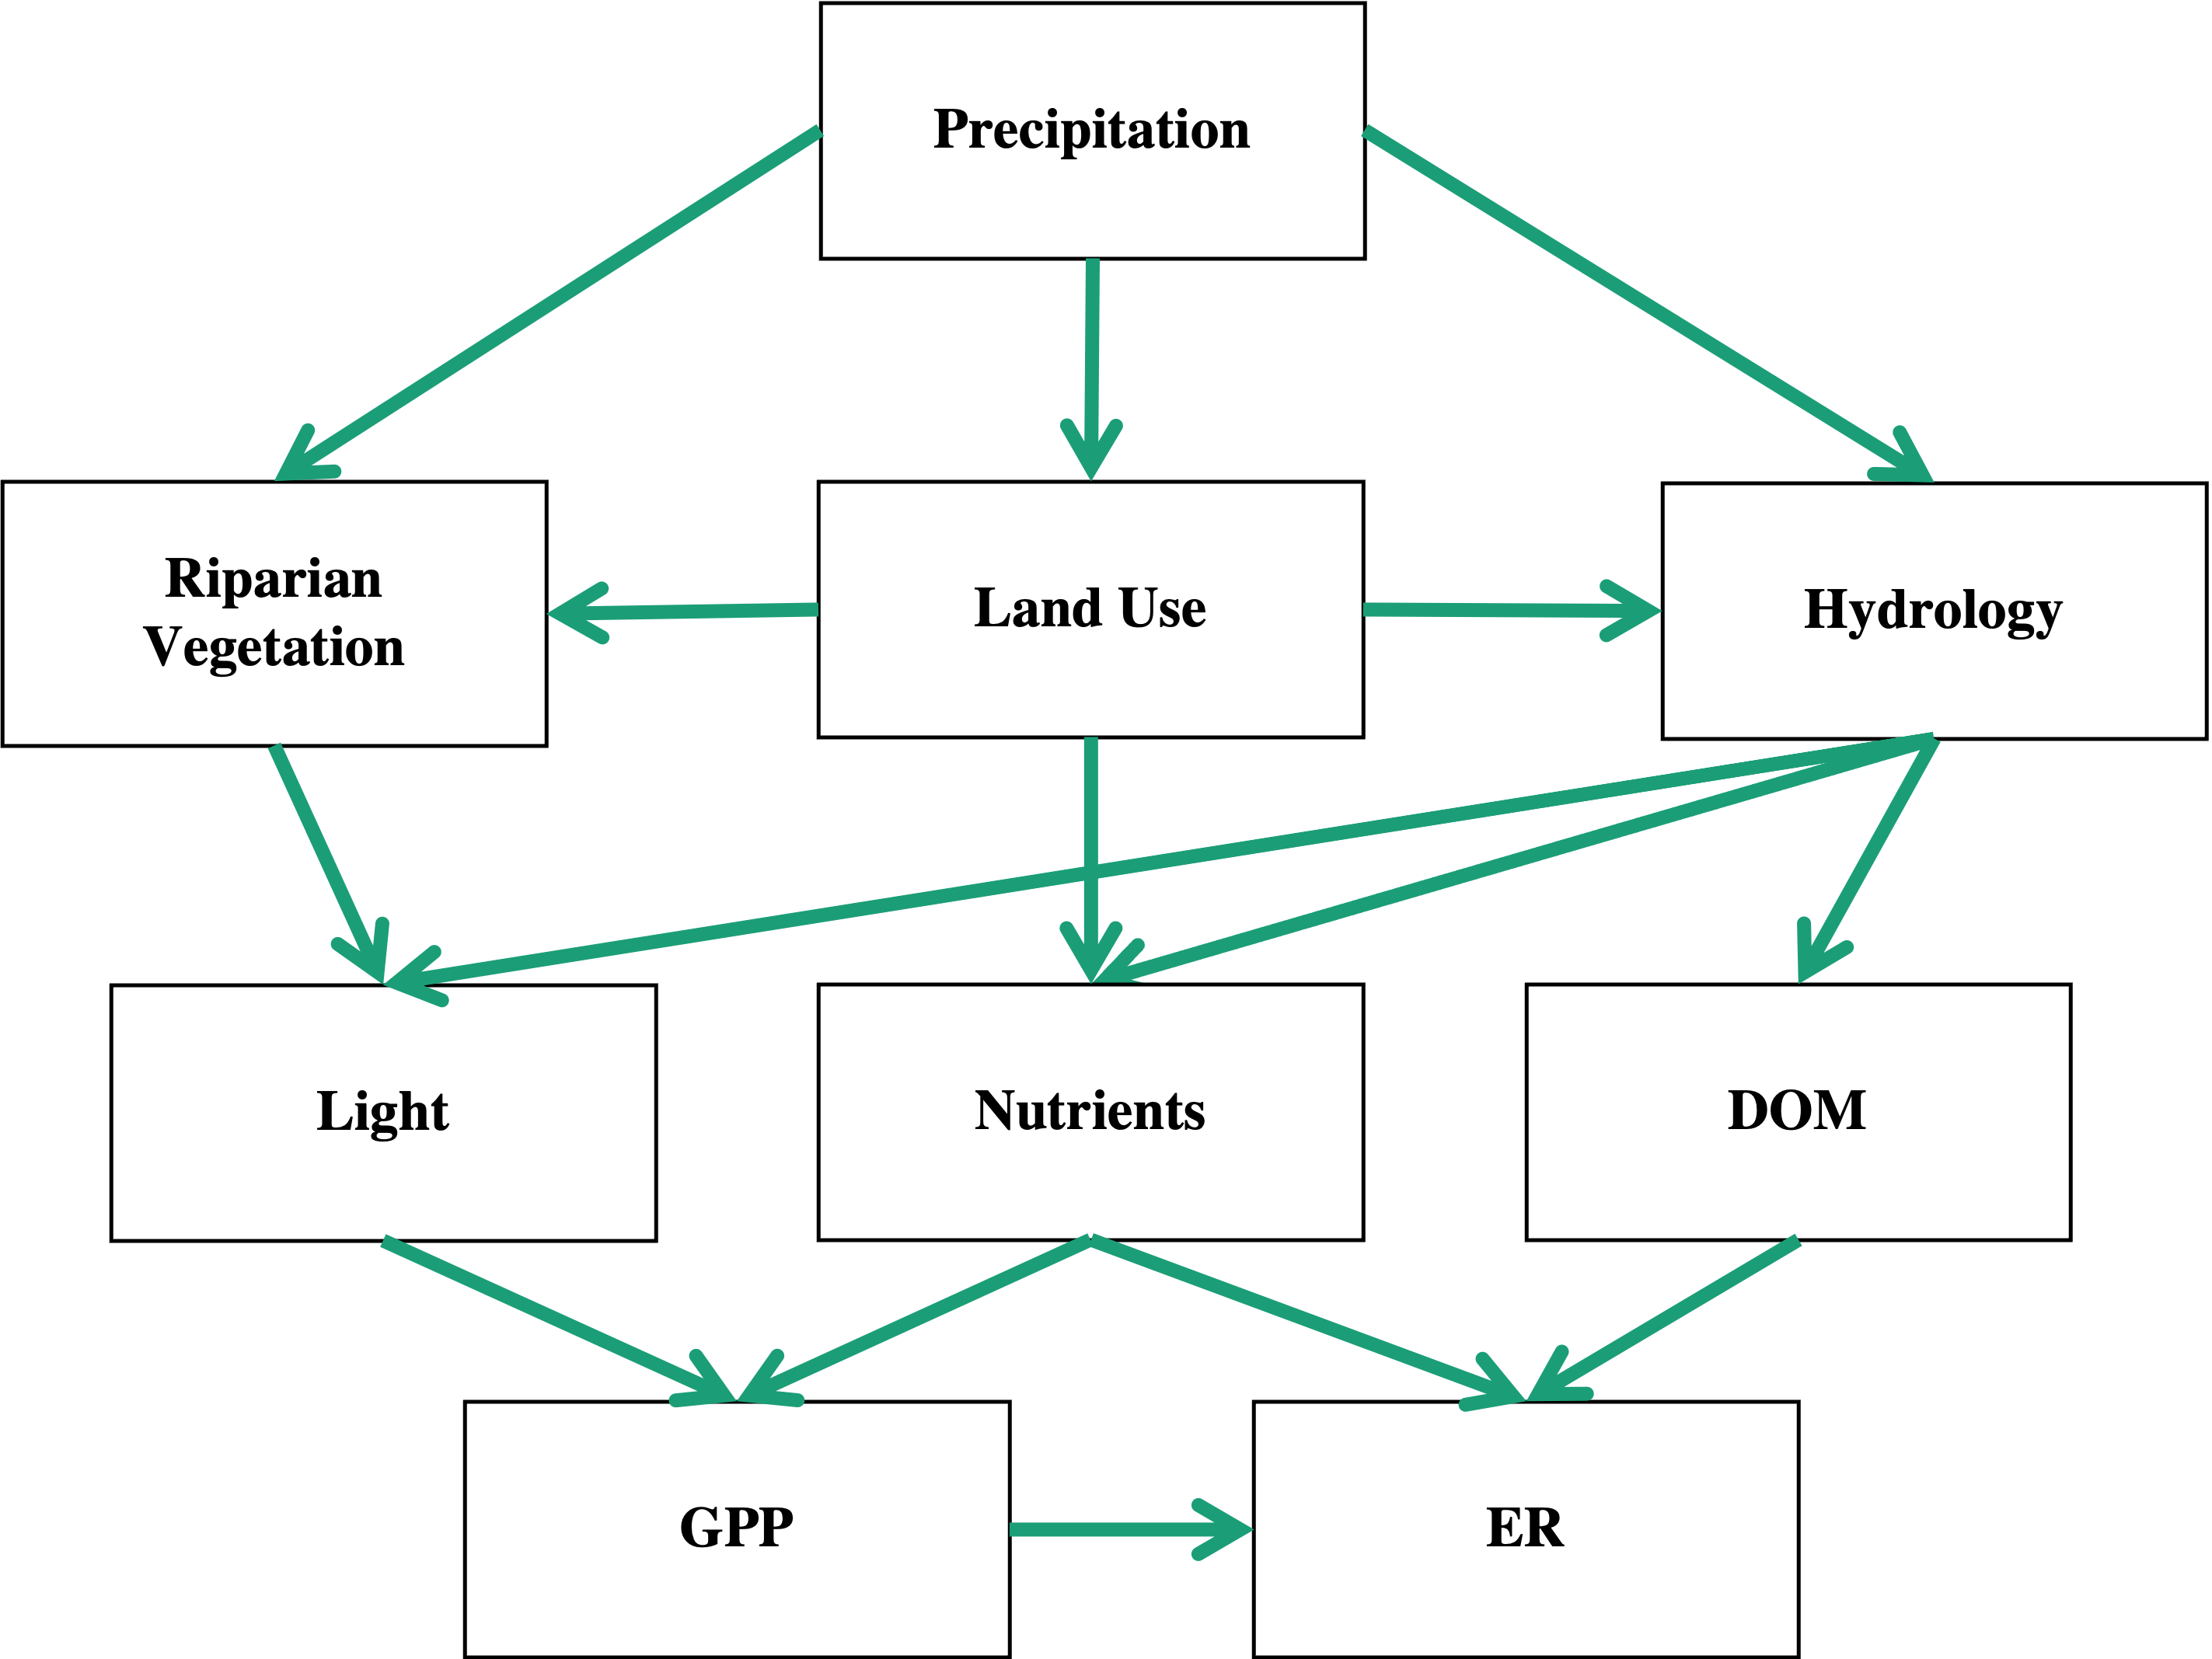
\includegraphics[scale=0.6]{Figs/ConceptDiagGREEN.png}
\caption[Conceptual Diagram]{\textit{Conceptual Diagram}. Conceptual diagram of hypothesized interactions between proximal and distal drivers on ecosystem metabolism.}
\label{fig:concept}
\end{center}
\end{figure}



\section{Research Questions}
\begin{enumerate}
    \item How do changes in light, nutrients, DOC, and hydrology that are driven by precipitation regimes drive patterns of ecosystem metabolism?
    \begin{itemize}
        \item Predictions:
         \begin{itemize}
        \item Increasing precipitation will cause high discharge, which will increase turbidity, attenuate light reaching the benthos, and suppress GPP.
        \item High discharge events will increase scouring or burying events and suppress GPP.
        \item High discharge events will dilute nutrient concentrations and suppress GPP and ER.
        \item As you move from arid to mesic, I expect DOC quantity to increase due to increased precipitation pulsing DOC from the watershed into the streams. Increased DOC will provide more fuel for microbes which will result in increased ER.
    \end{itemize}
    \end{itemize}

    \item How do changes in light, nutrients, DOC, and hydrology that are driven by changes in watershed land use drive patterns of ecosystem metabolism?
    \begin{itemize}
        \item Predictions:
        \begin{itemize}
        \item  Forested land that has been converted into agricultural land will have increased light availability from the removal of non-agricultural vegetation. This will drive an increase in both GPP and ER.
        \item  Forested land that has been converted into agricultural land will have increased nutrients from agricultural runoff, leading to an increase in GPP and ER.
        \item Non-agricultural vegetation will decrease light availability, resulting in suppressed GPP.
    \end{itemize}
    \end{itemize}
    
\end{enumerate}

         
         
         
         



  


\endinput

%-----------------------------------------------------------------------
% End of chap1.tex
%-----------------------------------------------------------------------


%-----------------------------------------------------------------------
% Beginning of chap2.tex
%-----------------------------------------------------------------------
%
%%%%%%%%%%%%%%%%%%%%%%%%%%%%%%%%%%%%%%%%%%%%%%%%%%%%%%%%%%%%%%%%%%%%%%%%

\chapter[METHODS]{Methods} 
\section{Study Areas}
To address my research questions, I analyzed nine Texas coastal plain streams falling along a precipitation, and subsequently, a land use gradient (Figure~\ref{Fig:PPT}~and~\ref{Fig:LandUse}). I estimated ecosystem metabolism in these streams from continuous measurements of dissolved oxygen and temperature for the time periods of 2017-2018 and 2020-2021.

Watershed areas for each of the nine sites were delineated from 1/3 arc-second digital elevation models (DEM) from the United States Geological Survey (USGS). I then calculated watershed land usage percentages using the National Land Cover Data-set (NLCD, 2019). All GIS analysis took place in ArcMap (Version 10.8, ESRI, USA) and QGIS (Version 3.22, QGIS Development Team, Switzerland).

\section{Site Descriptions}
The annual average precipitation along the coastal plain ranged from 55 cm~yr$^{-1}$ in the semi-arid to 135 cm~yr$^{-1}$ at the most mesic watershed along the 300 km precipitation gradient \cite{PRISM}. The catchment areas of the streams ranged from 73 to 1787 \unit{\square\km} (Table \ref{tab:WS Area}). Sites are characterized with high turbidity and intact riparian zones, ranging from dense forested canopy areas at the most mesic site to tall grasses at the most arid site (Figure~\ref{Pic:WMC}~and~\ref{Pic:TRC}). While these sites had intact riparian zones, watershed land use varied across sites following the precipitation gradient, from semi-arid to mesic, agriculture land use increased from 33\% to 82\%, while non-agricultural vegetation decreased from 55\% to 1\% (Figure~\ref{Fig:LandUse}). The precipitation gradient likely drove land use. A majority of sites had sandy substrate that mobilized during precipitation events. Substrate at other sites was composed of small pebbles and gravel. 

\begin{figure}[htb]
\begin{center}
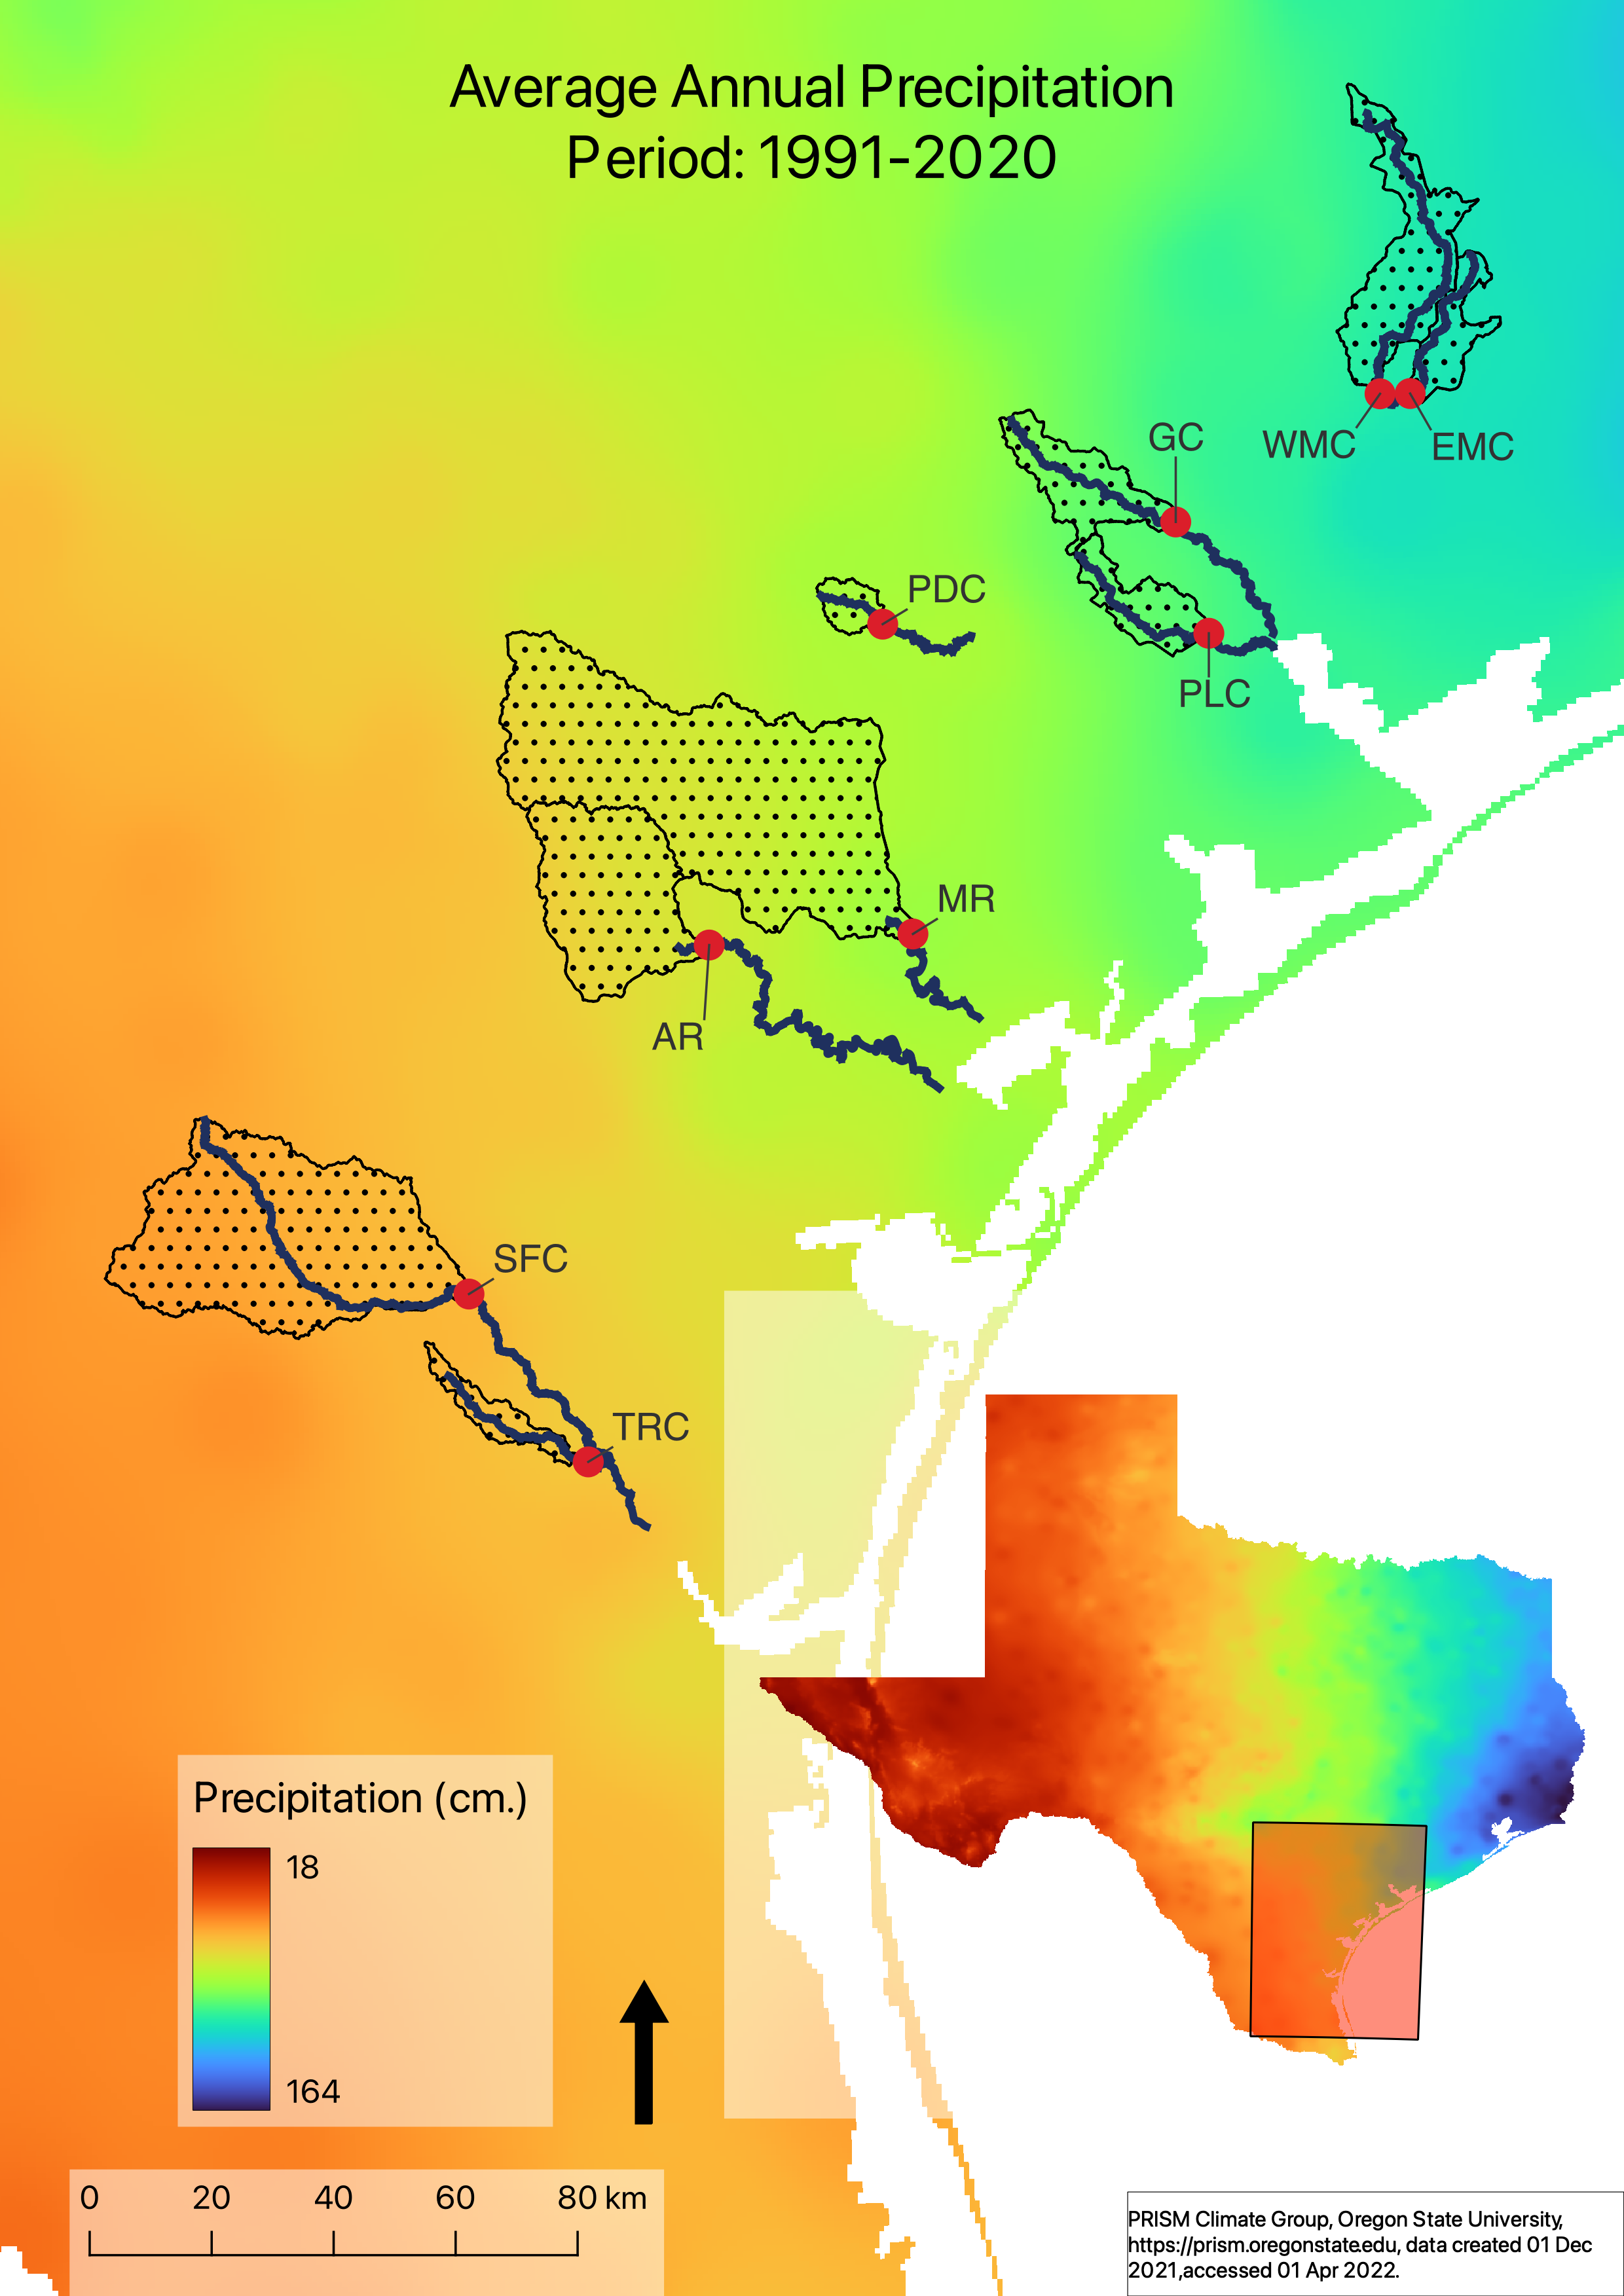
\includegraphics[scale = 0.7]{Figs/PPT.png}
\caption[Texas Precipitation Gradient]{\textit{Texas Precipitation Gradient.} The nine study sites and their watersheds across the 300 km coastal precipitation gradient.}
\label{Fig:PPT}
\end{center}
\end{figure}

\begin{landscape}
\begin{figure}[htb]
\begin{center}
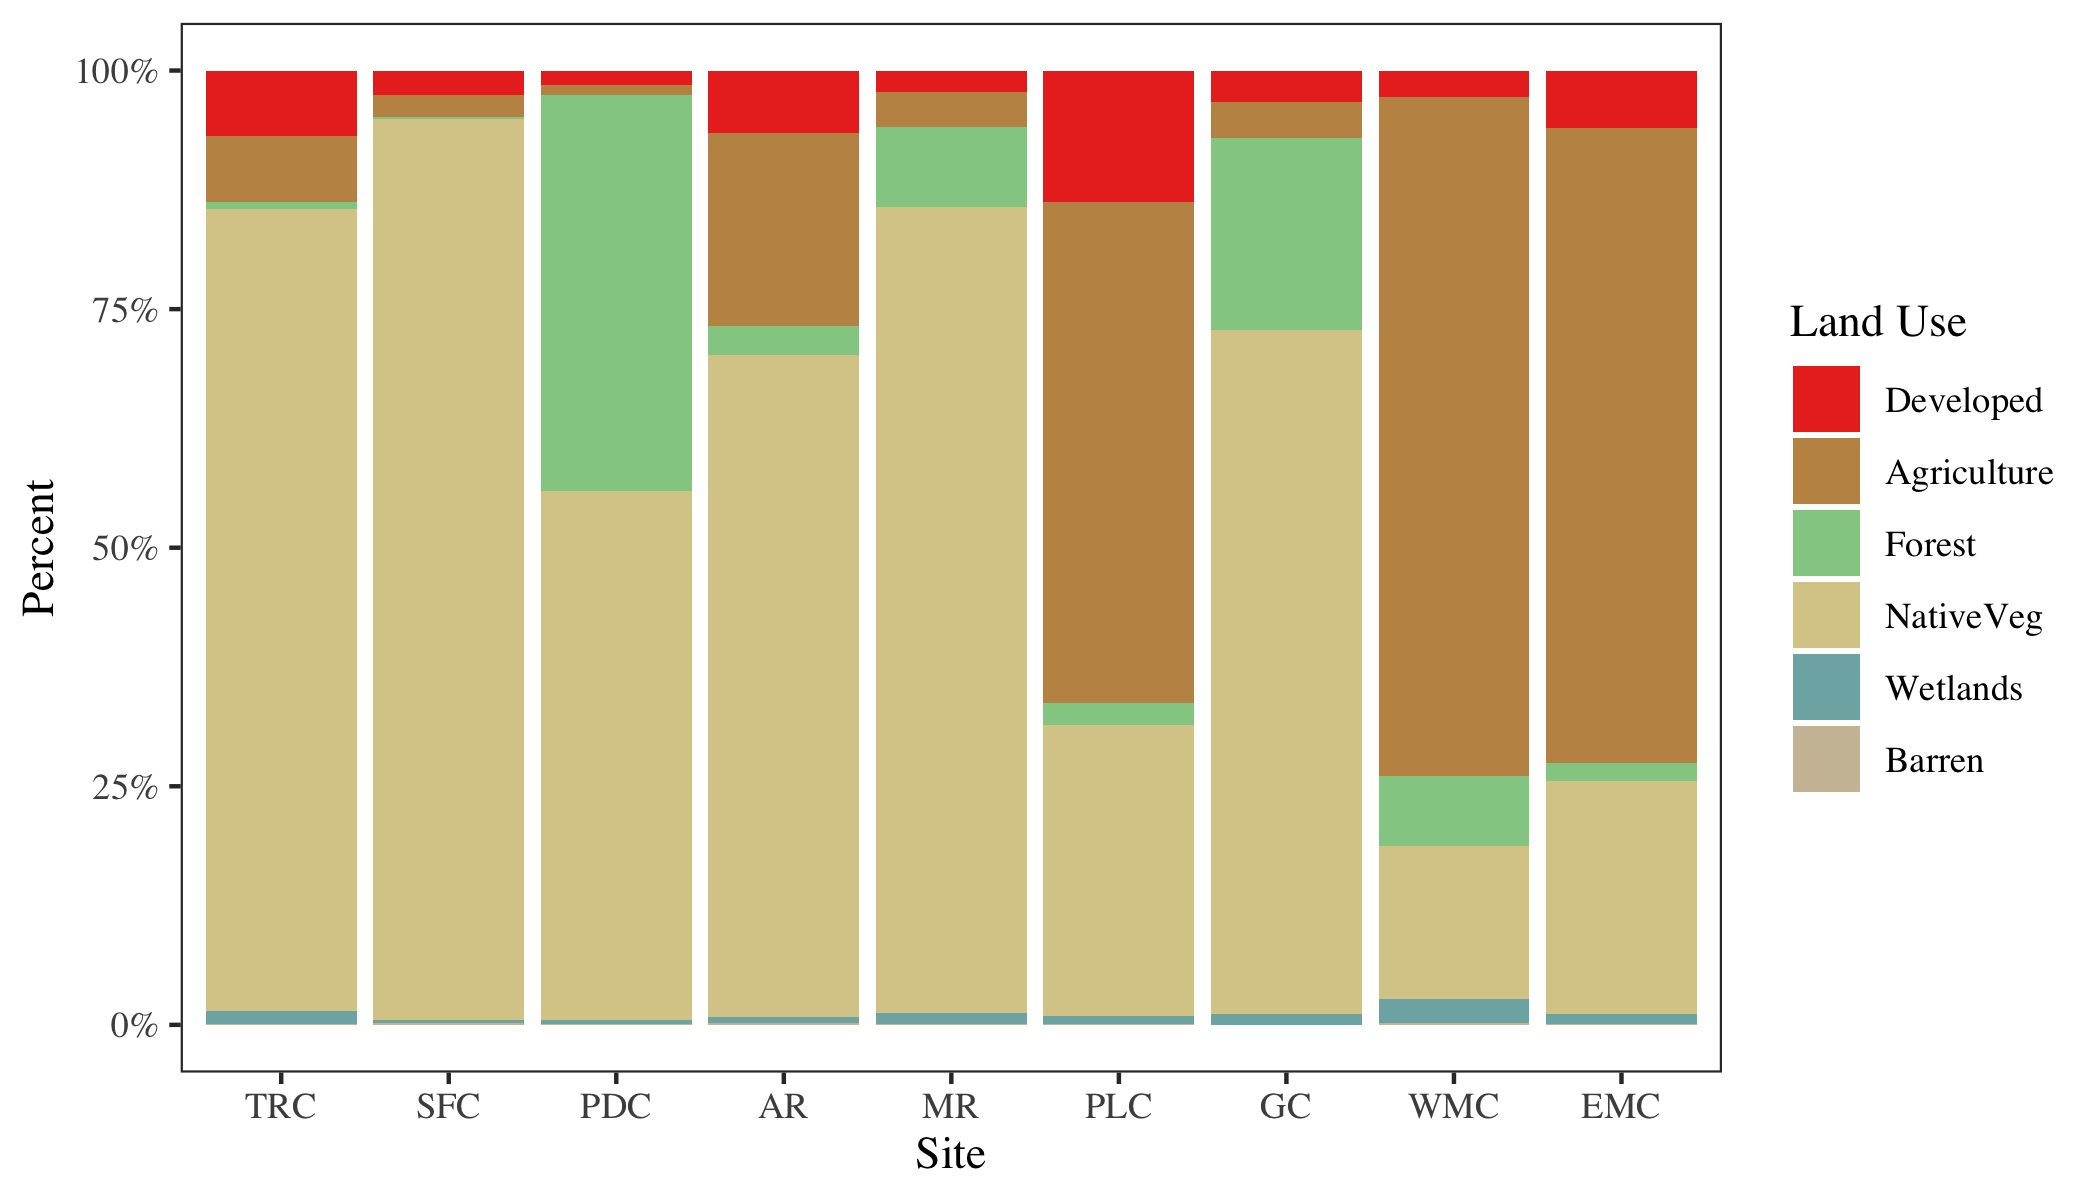
\includegraphics[scale=0.3]{Figs/LandUse.png}
\caption[Watershed Land Use]{\textit{Watershed Land Use.} Land cover types (\%) the nine study sites (Table \ref{tab:WS Area}). Sites are arranged from arid (left) to mesic (right).}
\label{Fig:LandUse}
\end{center}
\end{figure}
\end{landscape}

\begin{table}[htb]
\caption[Site Summary]{\textit{Site Summary}}
\begin{center}
\begin{tabular}
[c]{ccc}\hline
Site & Site Code & Watershed Area (\unit{\square\km})\\\hline
Tranquitas Creek & TRC & 126\\ 
San Fernando Creek & SFC & 1313\\ 
Aransas River & AR &  640 \\ 
Perdido Creek & PDC & 73 \\ 
Mission River & MR & 1787 \\ 
Placedo Creek& PLC & 177 \\ 
Garcitas Creek & GC & 273 \\ 
West Mustang Creek & WMC & 461\\ 
East Mustang Creek & EMC & 140\\\hline
\end{tabular}
\end{center}
\small \textit{Note}: Sites are arranged top to bottom, arid to mesic, with the site code. The largest watershed was 1787 \unit{\square\km}, while the smallest watershed was 73 \unit{\square\km}.
\label{tab:WS Area}
\end{table}

\begin{figure}[htb]
\begin{center}
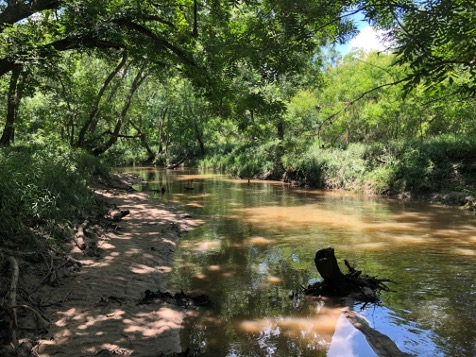
\includegraphics[scale = 0.8]{Figs/WMC.jpg}
\caption[WMC]{\textit{WMC.} This site is one of the most mesic sites and is characterized with high turbidity, high canopy cover, that likely decreases light availability, and sandy substrate.}
\label{Pic:WMC}
\end{center}
\end{figure}

\begin{figure}[htb]
\begin{center}
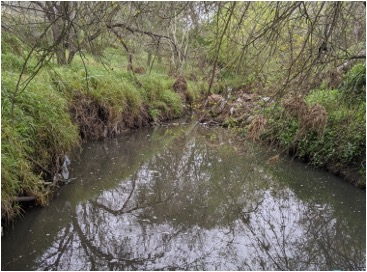
\includegraphics[scale = 0.8]{Figs/trc.jpg}
\caption[TRC]{\textit{TRC.} This site is the most arid site and is characterized with high turbidity and dense riparian vegetation, likely decreasing light availability.}
\label{Pic:TRC}
\end{center}
\end{figure}


\section{Ecosystem Metabolism}

I estimated daily GPP and ER from continuously measured dissolved oxygen concentrations using a one-station approach \cite{odum_primary_1956}. In one-station models, dissolved oxygen (DO) concentrations are used to estimate GPP, ER, and K$_O$ (gas exchange rate [\unit{\per\day}] for oxygen at stream water temperature). DO and temperature were measured every 10 minutes with miniDOT (PME) DO loggers in the stream thalweg, to ensure the water was well mixed. I used the R package StreamLight \cite{savoy_streamlight_2021}, this package uses NLDAS, LAI, and field measurements to estimate light for each site.  GPP, ER, and K$_O$ were modeled using the R package streamMetabolizer  \cite{appling_streammetabolizer_2018}. I used high frequency DO, temperature, and PAR to estimate GPP, ER, and K$_O$ using the following equation \cite{hotchkissHighRatesDaytime2014, hall_turbidity_2015, ulseth_climate-induced_2018, hall_gas_2019}:
\begin{equation*}\label{metab}
\text{O}_{i}=\text{O}_{i-\Delta t}+\left(\left(\frac{\text{GPP}_{d}}{\bar{Z}} \times \frac{\text{PAR}_{i}}{\sum \text{PAR}_{d}}\right)+\frac{\text{E R}_{d}}{\bar{Z}}+\text{K}_{o}\left(\text{O}_{{\text{sat}}(i-\Delta t)}-\text{O}_{i-\Delta t}\right)\right) \Delta t
\end{equation*}
Where O$_i$ is the DO (\unit{\mg\per\l}) concentration at time $i$ and and $O_{(i-\Delta t)}$ is the DO concentration at the time step prior to $O_i$ and $\Delta t$ is the time-step of the analysis (10 minutes). GPP$_d$ and ER$_d$ are areal fluxes of GPP and ER for day $d$ (\unit{\goxy}). $\bar{Z}$ is daily average stream reach depth (m). The gas exchange rate, K$_O$ is at stream water temperature. DO at saturation, O$_{sat}$ refers to oxygen concentration (\unit{\mg\per\l}) at 100\% saturation at stream water temperature and barometric pressure \cite{garcia_oxygen_1992}, which was measured at the Texas A\&M University—Corpus Christi Meteorological station (27° 42' 54" N, 97° 19' 43" W). PAR$_i$ (\unit{\umol} \unit{\per\square\m\per\s}) is photosynthetic active radiation at time $i$ calculated using a function in streamMetabolizer \cite{appling_streammetabolizer_2018} and $\sum$ PAR$_d$, is the light intensity for day $d$.


The Bayesian model from streamMetabolizer was used to estimate GPP, ER, and K$_{600}$, the gas exchange coefficient, normalized to normalized to a Schmidt number of 600. I used partial pooling of K$_{600}$ across all days from each site. The model was run for 2000 warm up steps and then 2000 saved steps, to ensure the Bayesian chains converge \cite{appling_metabolic_2018, arroita_twenty_2019}. The Baysian model was run with 4 chains, on 4 cores in parallel. 

I used several criteria to evaluate model fit. First, I used the relationship between ER and K$_{600}$, if ER and K$_{600}$ are strongly related the model did not fit, then days where K$_{600}$ exceeded 100 were thrown out, these are very high values and likely not plausible given the low slope and low turbulence of these coastal plain streams. Days with high stream flow (+ 2 SD) were also removed from the model, high stream flow results in a dilution of the diel oxygen signal, which becomes problematic when trying to estimate GPP, ER, and K$_{600}$. Additionally, when DO was equal to or less than 0.01 \unit{\mg\per\l}, these days were thrown out as this is when sensors were believed to be buried under sediment after large rain events. 


\section{DOC and Nutrients}
I collected water samples monthly to quantify nutrient (NO$_3$-N, NH$_4$-N, and PO$_4$-P) and DOC concentrations. I filtered water from each site with a \qty{0.7}{\um} pre-combusted glass fiber filter (GFF) into acid-washed 60 mL nalgene bottles for nutrients and acid-washed pre-combusted 40 mL glass vials for DOC for a total of 4 replicates for both nutrients and DOC. All samples were kept cold and in the dark until transported to the laboratory. Nutrient samples were frozen until analysis at Oklahoma State University Soil, Water and Forage Analytical Laboratory. DOC concentrations were measured using a Shimadzu TOC/TN analyzer at Sam Houston State University.  

\section{Discharge}
To characterize discharge and calculate average reach depth, field measurements of width, velocity, and gage measurements of discharge were retrieved from the United States Geological Survey. Using relationships of depth and discharge from each site, I calculated daily average stream depth, these measurements were then used as $\bar{Z}$, daily average stream reach depth (m), in the equation above \cite{dataRetrival, surveyUSGSWaterData1994, raymond_scaling_2012}

\section{Statistical Analysis}


To quantify the effect of land use and the precipitation gradient on ecosystem metabolism, I used structural equation modeling (SEM) to test my hypotheses (Figure~\ref{fig:concept}) \cite{bernot_inter-regional_2010, fus_land_2017}. SEMs are used when there is an underlying mechanism that is causing co-variance between random variables, it also take into account correlated independent variables, measurement error, and provides a more robust analysis compared to multivariate approaches \cite{malaeb_using_2000, bernot_inter-regional_2010}. To group land use categories for the structural equation model, I used a principal components analysis (PCA) \cite{rcore}. The two land use PCs were used in the structural equation model as a proxy for land use. I included log-transformed monthly estimates of GPP, ER, DOC concentration, and turbidity, monthly averages of NO$_3$-N, PO$_4$-P, precipitation, and discharge. I used Standardized Root Mean Square Residual (SRMR) to compare model fit. Statistical analysis was preformed with R version 4.1.0 and lavaan \cite{rcore, rosseel_lavaan}.

\endinput

%-----------------------------------------------------------------------
% End of chap2.tex
%-----------------------------------------------------------------------


%-----------------------------------------------------------------------
% Beginning of chap3.tex
%-----------------------------------------------------------------------
%
%%%%%%%%%%%%%%%%%%%%%%%%%%%%%%%%%%%%%%%%%%%%%%%%%%%%%%%%%%%%%%%%%%%%%%%%

\chapter[RESULTS]{Results}
\vspace{-12pt}
\section{Ecosystem Metabolism}

Across all sites, median GPP ranged from 0.12 to 0.77 \unit{\goxy}, while median ER ranged -0.84 to -10.85 \unit{\goxy}. ER exceeded GPP across all sites, resulting in median NEP ranging from -0.35 to -10.41 \unit{\goxy} (Table \ref{tab:GPP-ER}). All sites were heterotrophic, i.e, where ER exceeds GPP, with very few (1-4) autotrophic days. Across all sites, day to day variability in GPP (CV 1.16 \%) was low whereas ER (CV -1.18 \%) exhibited slightly more daily variation than GPP (Figure~\ref{fig:GPPvER}). There was a subtle increase in GPP across the precipitation gradient, with the exception of GC where median GPP was low (0.25 \unit{\goxy}), falling in line with the most arid sites (Figure~\ref{fig:GPPBox}). 

Unlike GPP, there was no discernible pattern in ER (Figure~\ref{fig:ERBox}) nor in NEP (Figure~\ref{fig:NEPBox}) from semi-arid to mesic study sites. ER varies across the precipitation gradient, but ER at WMC  was 3-13 fold greater than the other sites (Table~\ref{Tab:GPPandER}). At PDC, I was only able to estimate metabolism for 279 days out of the nearly 2 years of data because the stream was completely dry or was disconnected pools during 2020-2021 (Table~\ref{Tab:GPPandER}).


Between SFC, AR, and PLC there appeared to be slight spring and summer increases in GPP and ER across the precipitation gradient in 2020, there is not the same pattern in 2017. GPP increased later into the summer as precipitation increased along the gradient (Figure~\ref{Fig:MetabStacked}).

\begin{figure}[htb]
\begin{center}
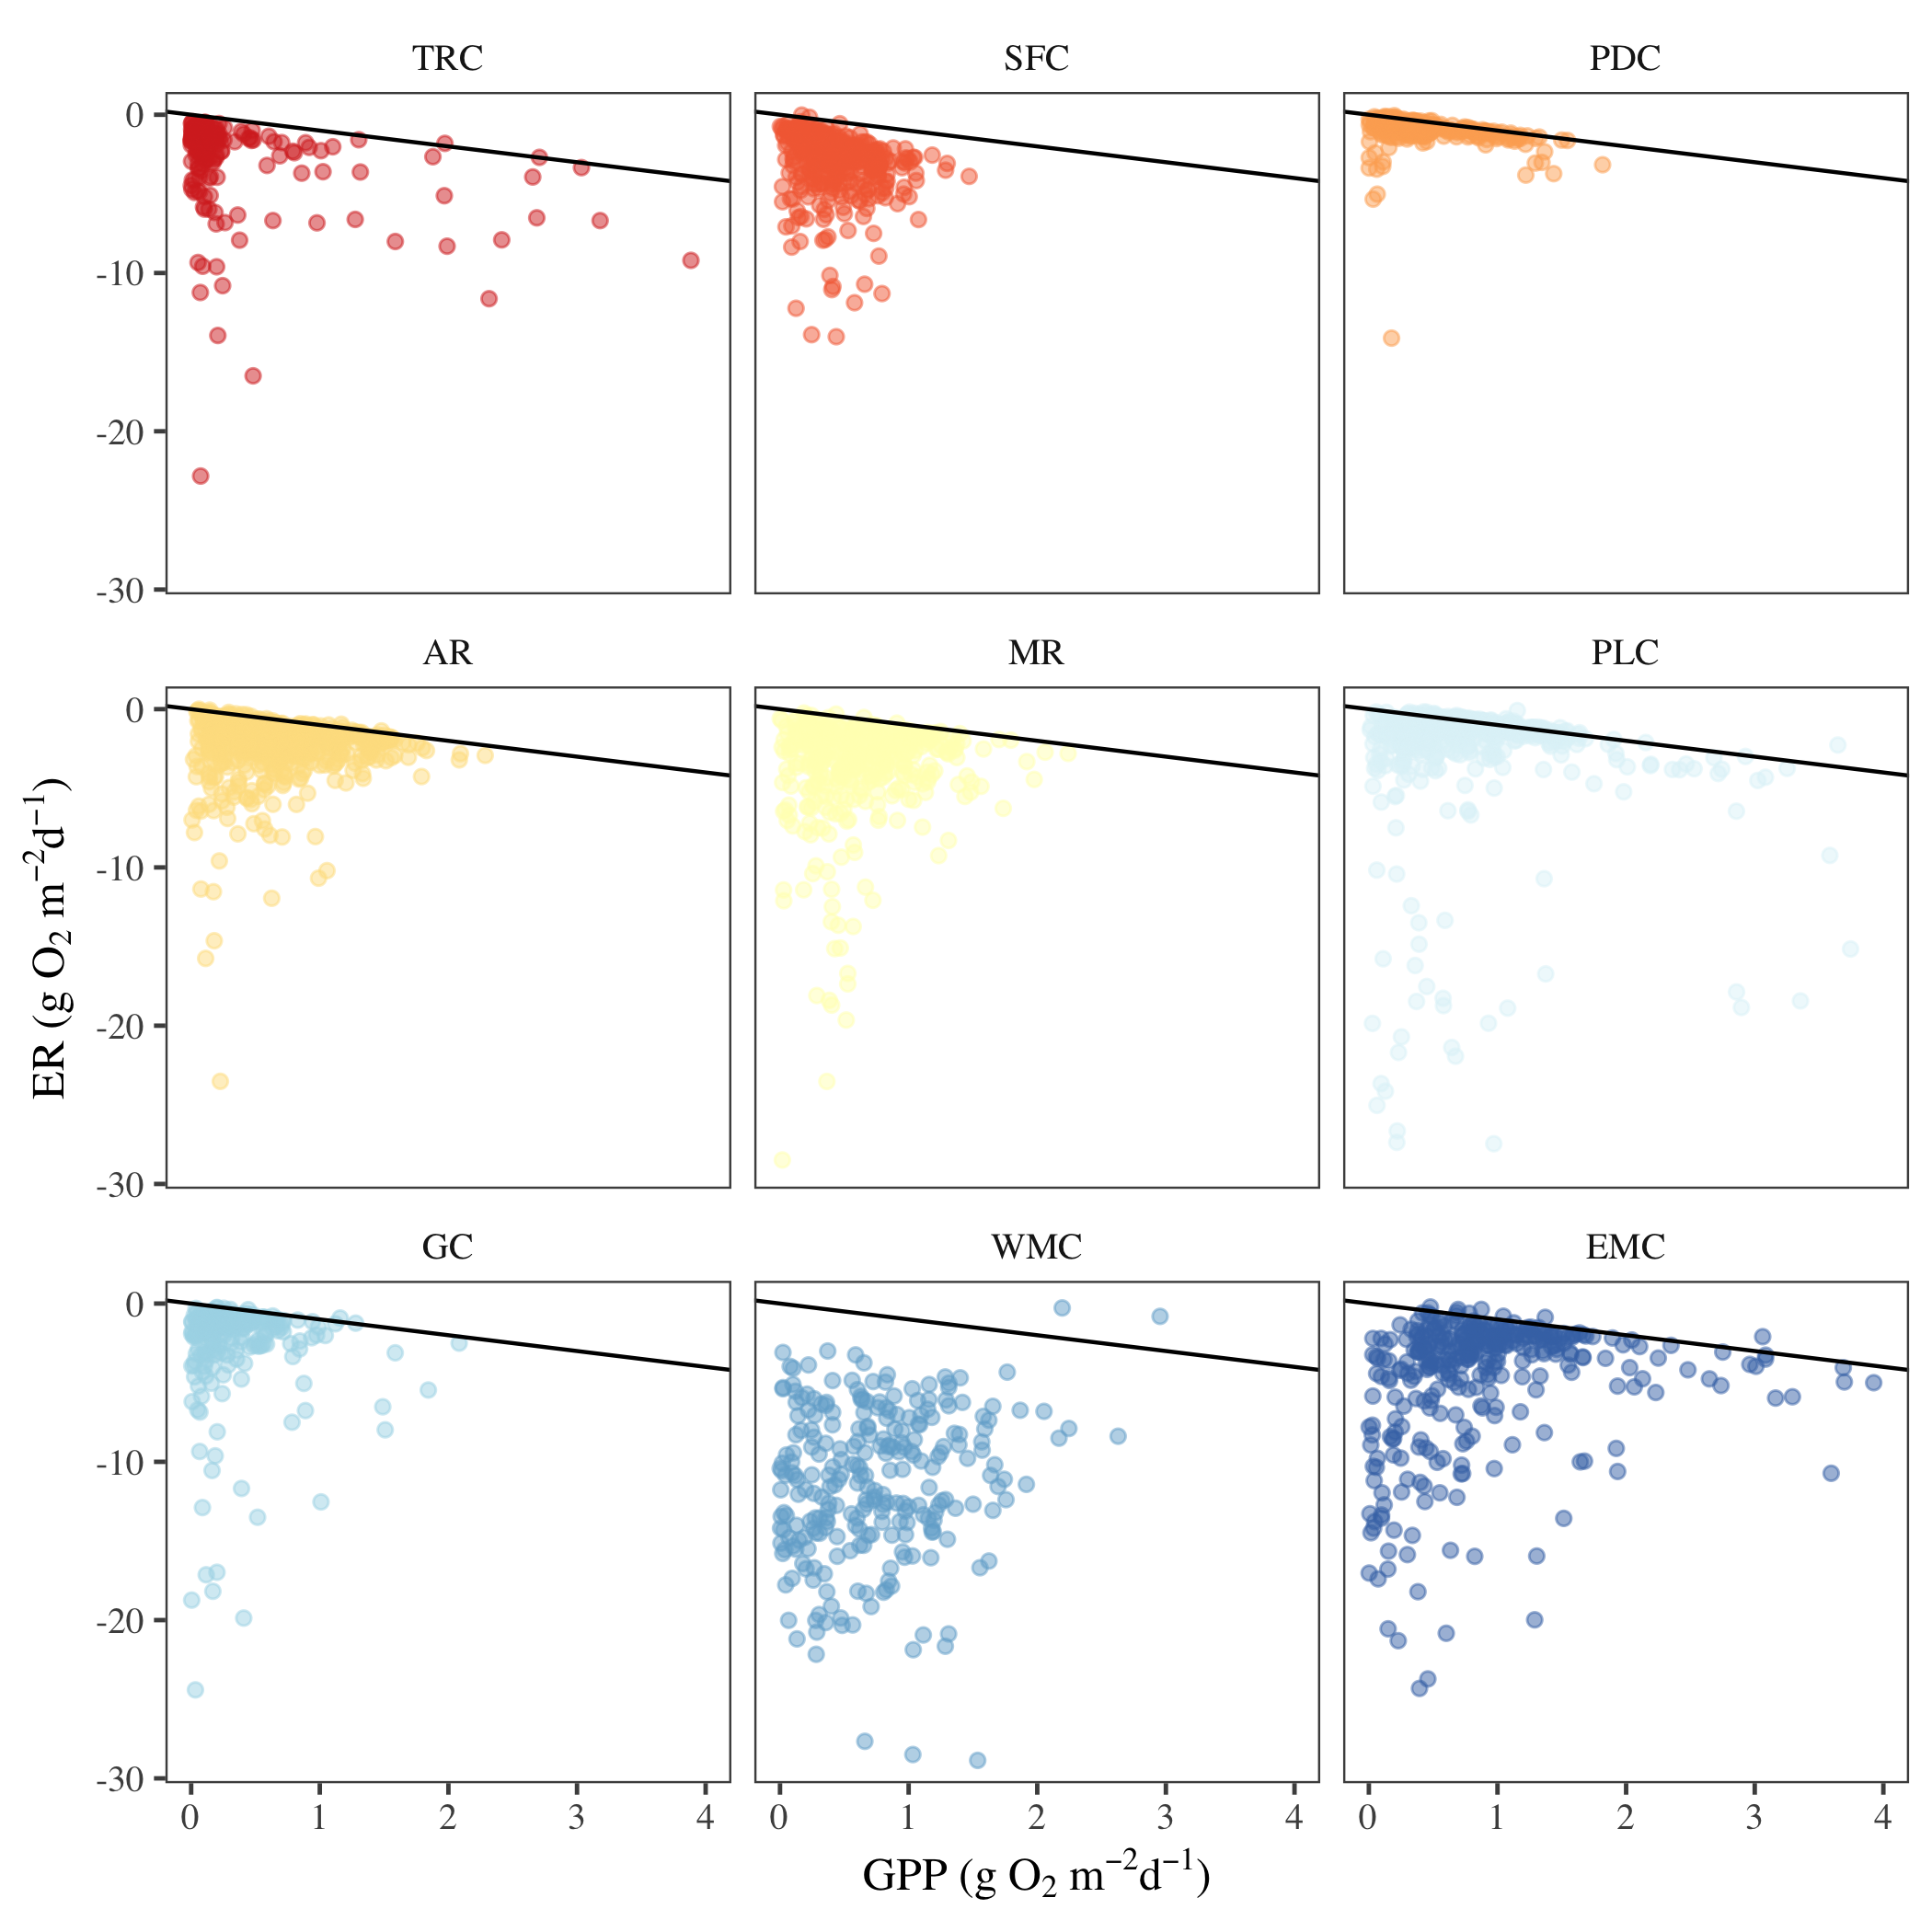
\includegraphics[scale=0.2]{Figs/GPPvER.png}
\caption[Gross Primary Production and Ecosystem Respiration]{\textit{Gross Primary Production and Ecosystem Respiration}. Sites are arranged from arid to mesic left to right and top to bottom (red to blue). Points above the 1:1 line indicate days of autotrophy where gross primary production (GPP) exceeds ecosystem respiration (ER), and points below are heterotrophic days were ER exceeds GPP. Across all sites, ER was more variable than GPP with very few autotrophic days (e.g. 2 days at WMC and 1 day at PLC and EMC).}
\small 
\label{fig:GPPvER}
\end{center}
\end{figure}

\begin{figure}[htb]
\begin{center}
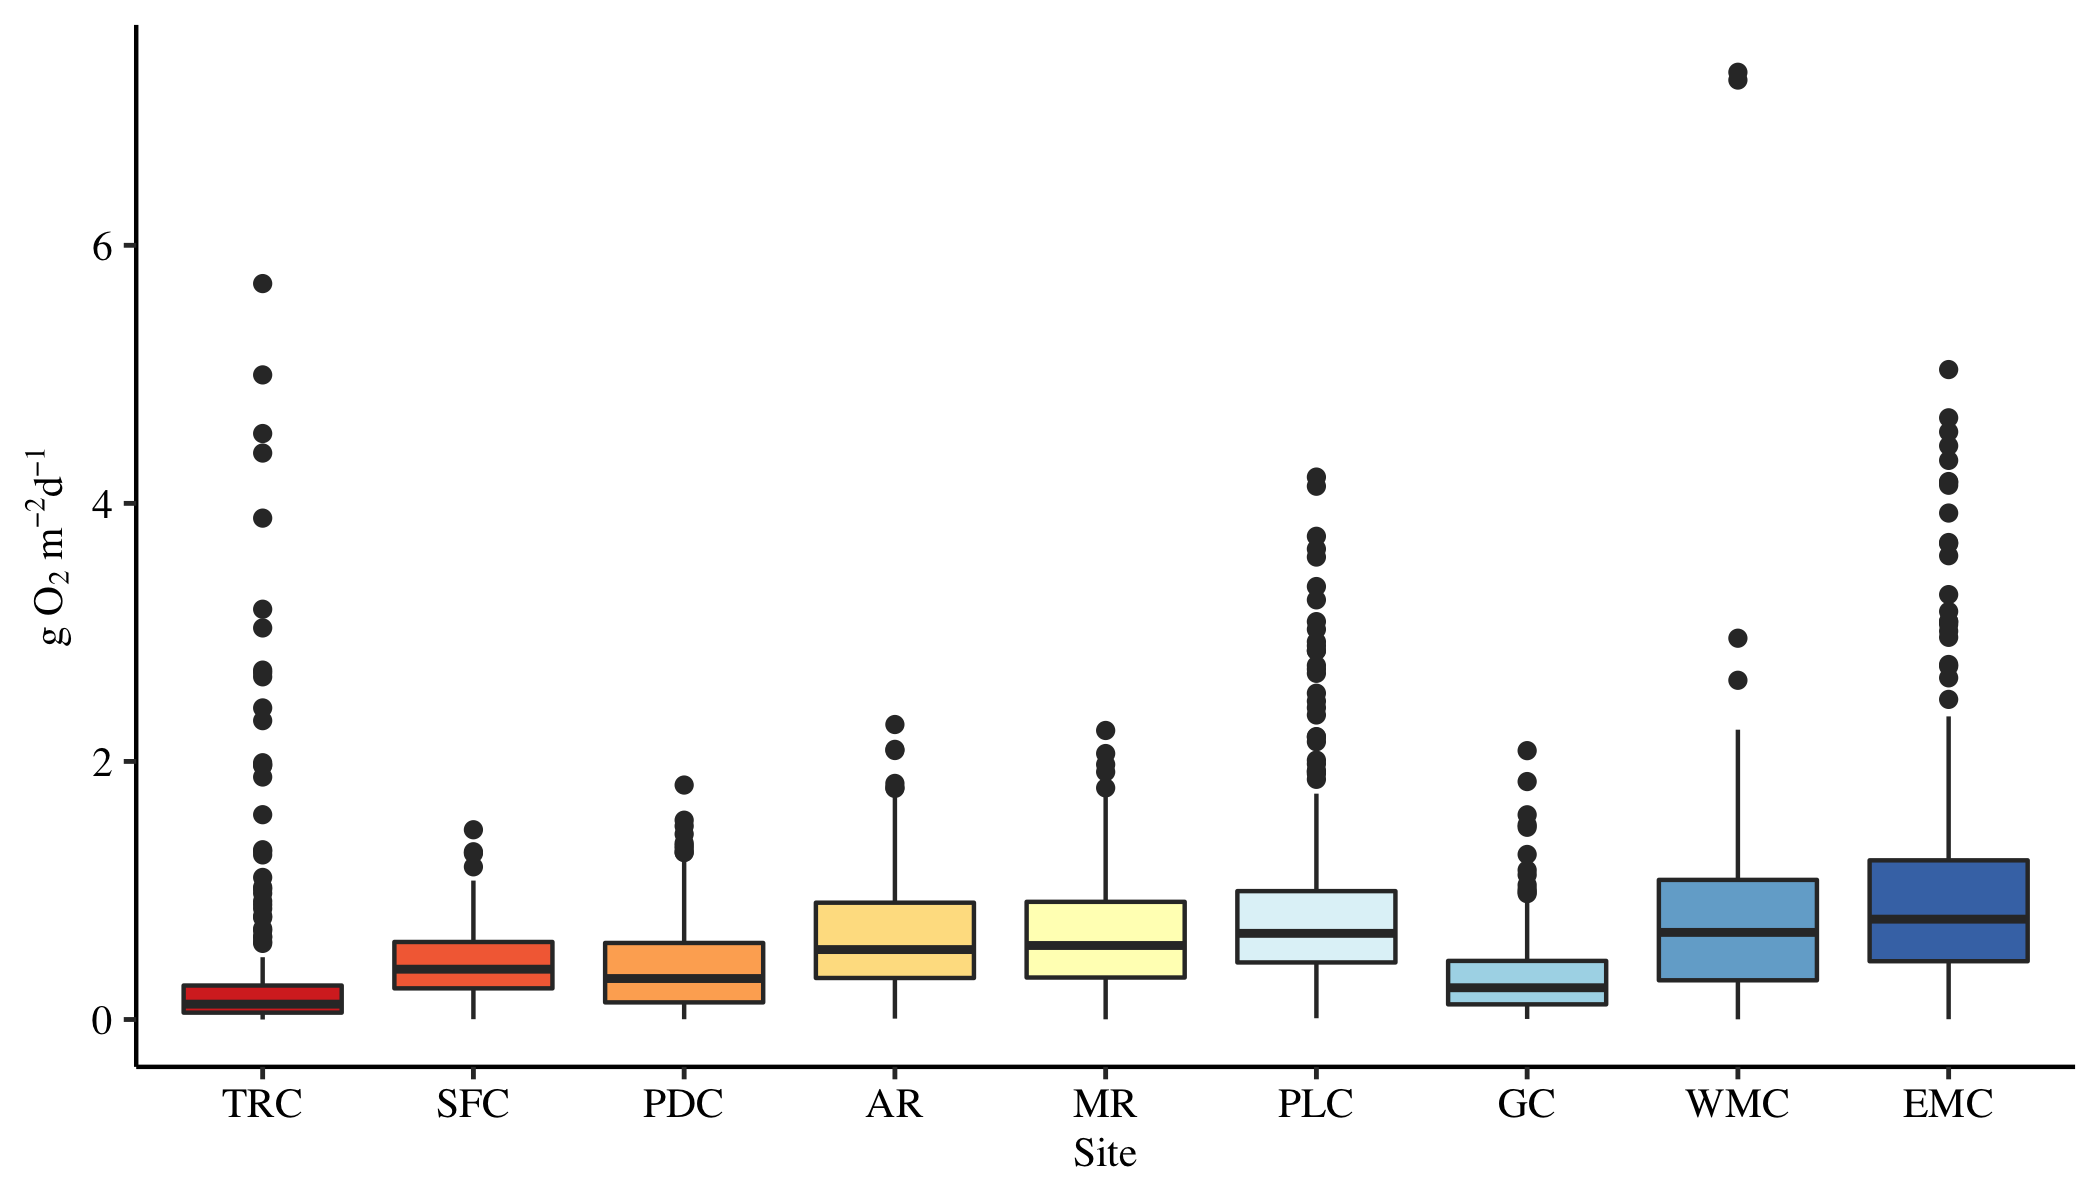
\includegraphics[scale=0.2]{Figs/GPPBox.png}
\caption[Gross Primary Production]{\textit{Gross Primary Production}. There was a subtle increase in GPP across the precipitation gradient (sites are arranged arid to mesic, left to right), with the exception of GC, falling in line with the most arid sites. The boxes are the middle 50 quartile (25 to 75), the line is the median, the tails are 1.5X interquartile range, and any points falling outside of the line are considered outliers.}
\label{fig:GPPBox}
\end{center}
\end{figure}

\begin{figure}[htb]
\begin{center}
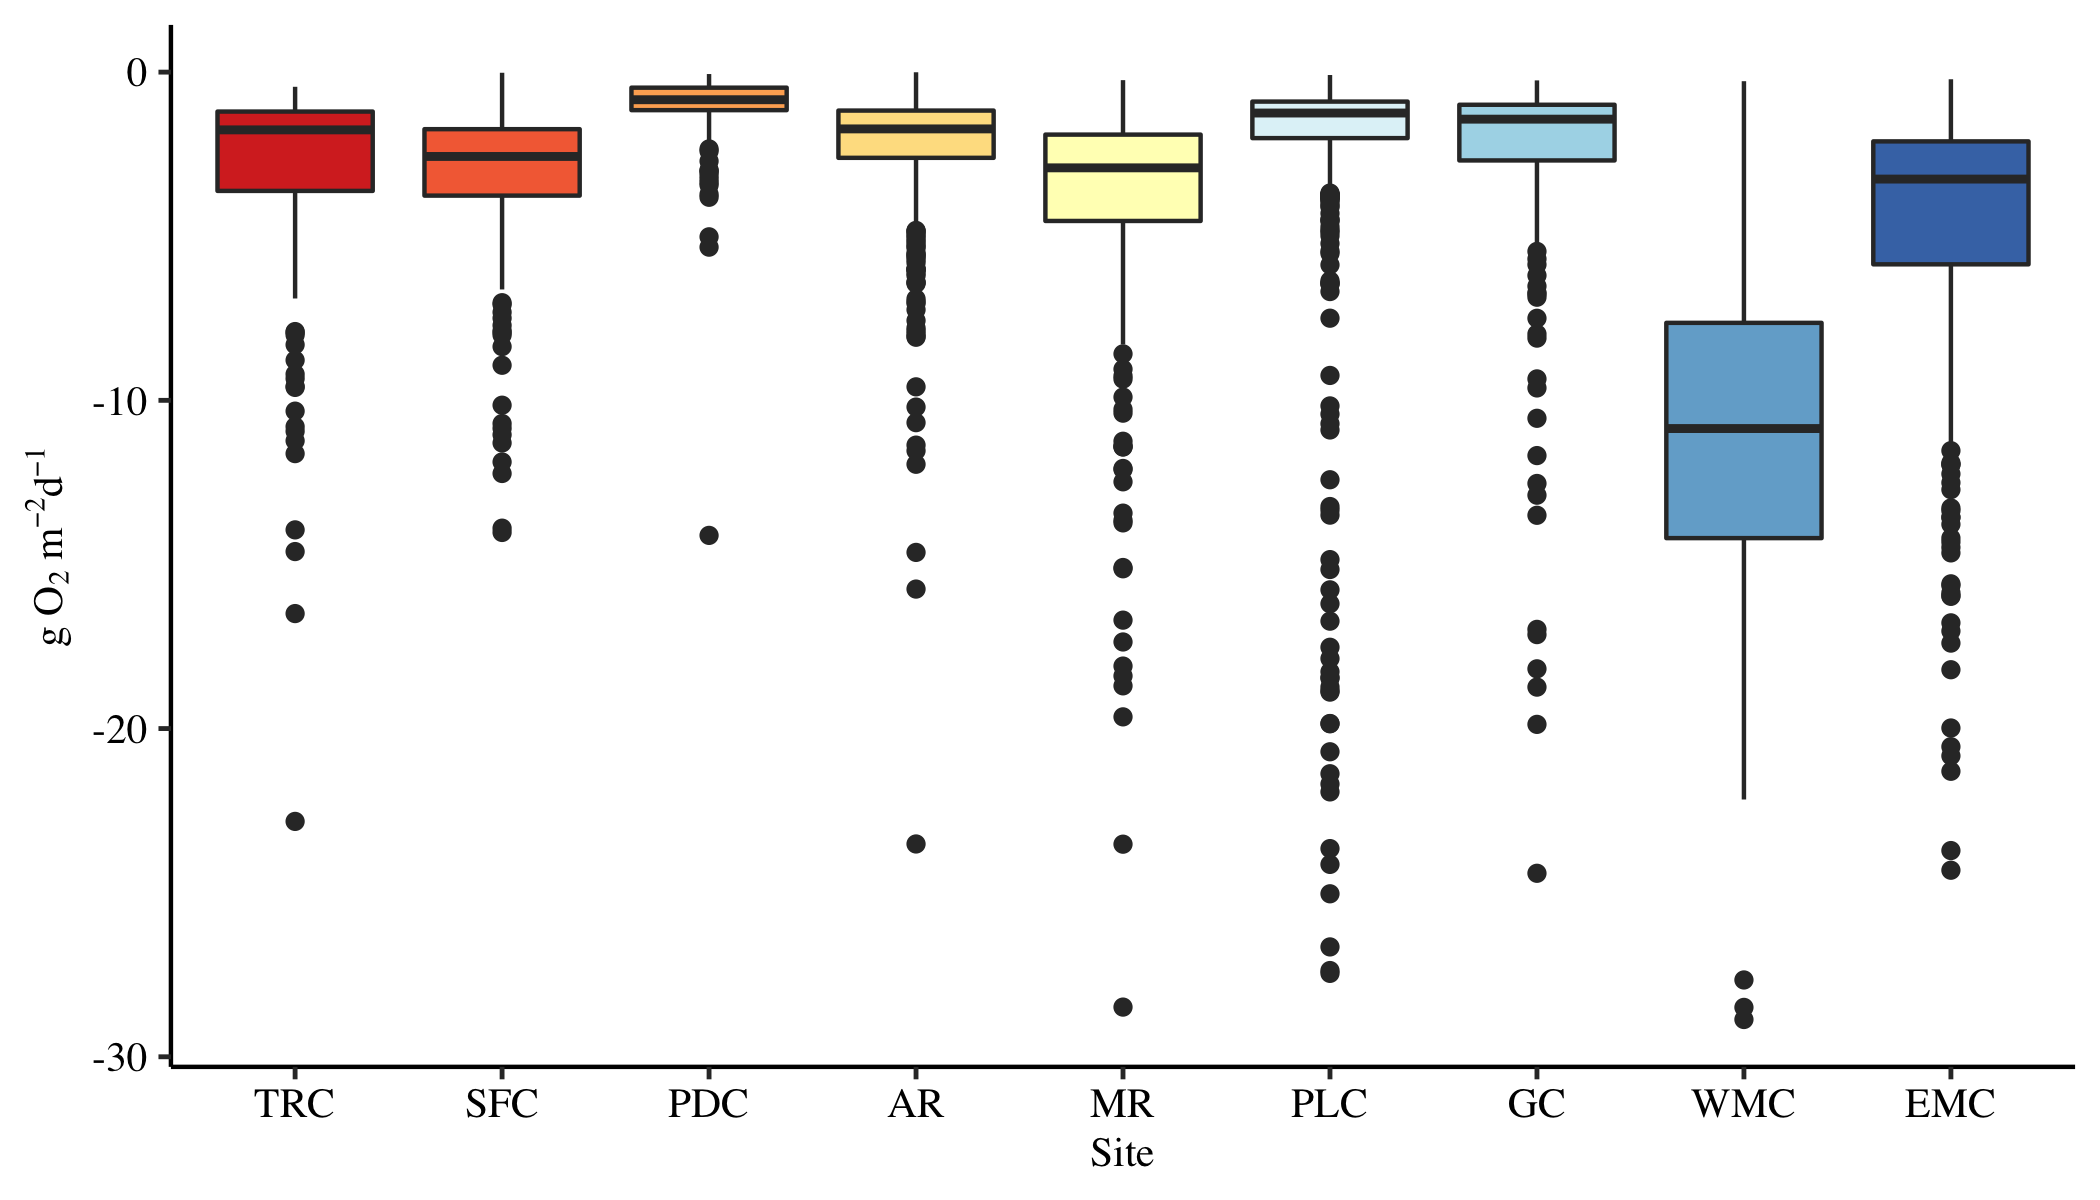
\includegraphics[scale=0.2]{Figs/ERBox.png}
\caption[Ecosystem Respiration]{\textit{Ecosystem Respiration}. There appears to be no discernible pattern in ecosystem respiration (ER) along the precipitation gradient (sites are arranged arid to mesic, left to right). The boxes are the middle 50 quartile (25 to 75), the line is the median, the tails are 1.5X interquartile range, and any points falling outside of the line are considered outliers.}
\label{fig:ERBox}
\end{center}
\end{figure}

\begin{figure}[htb]
\begin{center}
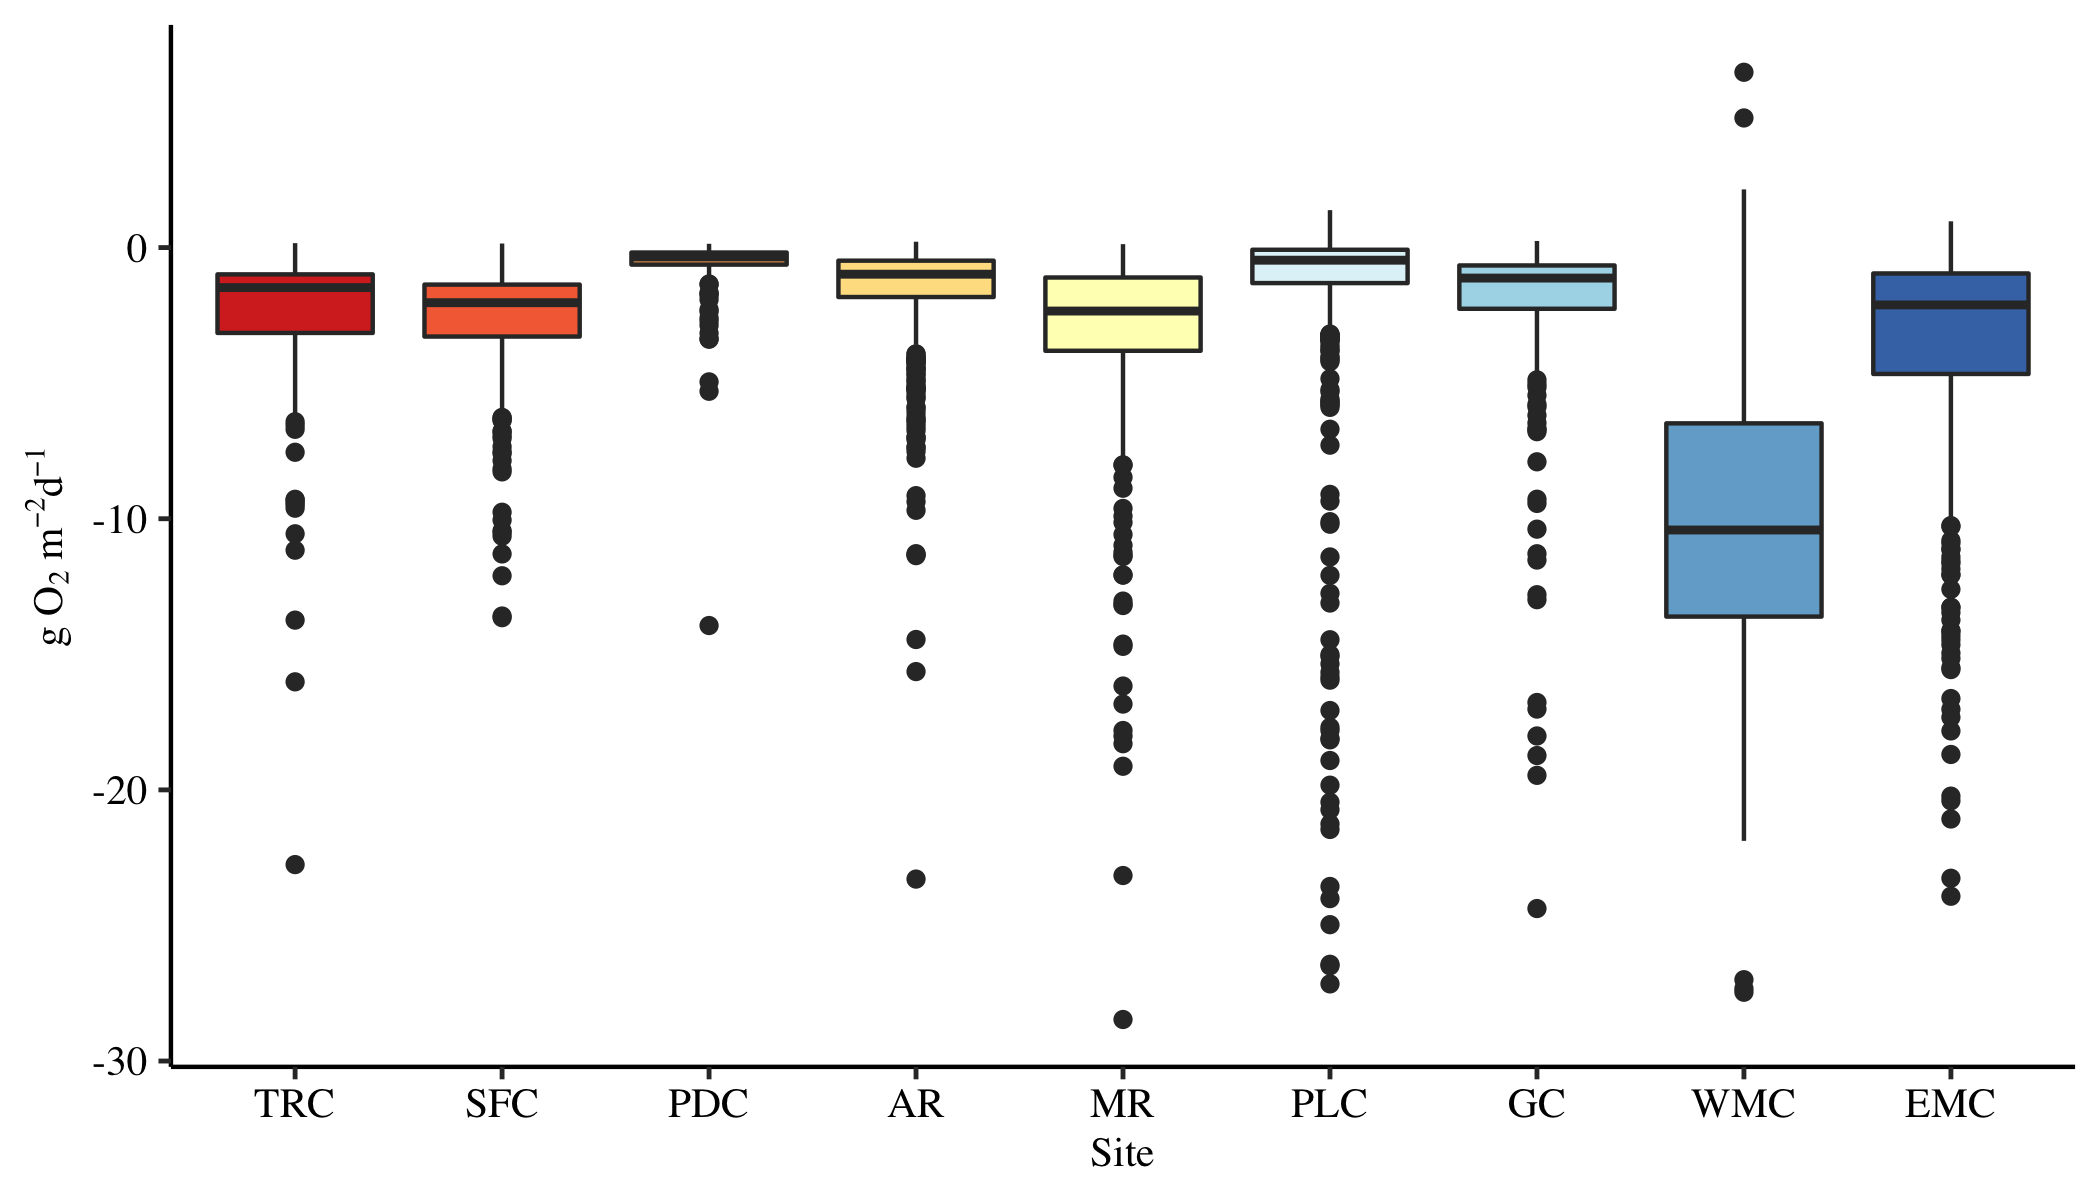
\includegraphics[scale=0.2]{Figs/NEPBox.png}
\caption[Net Ecosystem Production]{\textit{Net Ecosystem Production}. There appears to be no discernible pattern in net ecosystem production (NEP) along the precipitation gradient (sites are arranged arid to mesic, left to right). The boxes are the middle 50 quartile (25 to 75), the line is the median, the tails are 1.5X interquartile range, and any points falling outside of the line are considered outliers.}
\label{fig:NEPBox}
\end{center}
\end{figure}

\begin{landscape}
\begin{figure}[htb]
\begin{center}
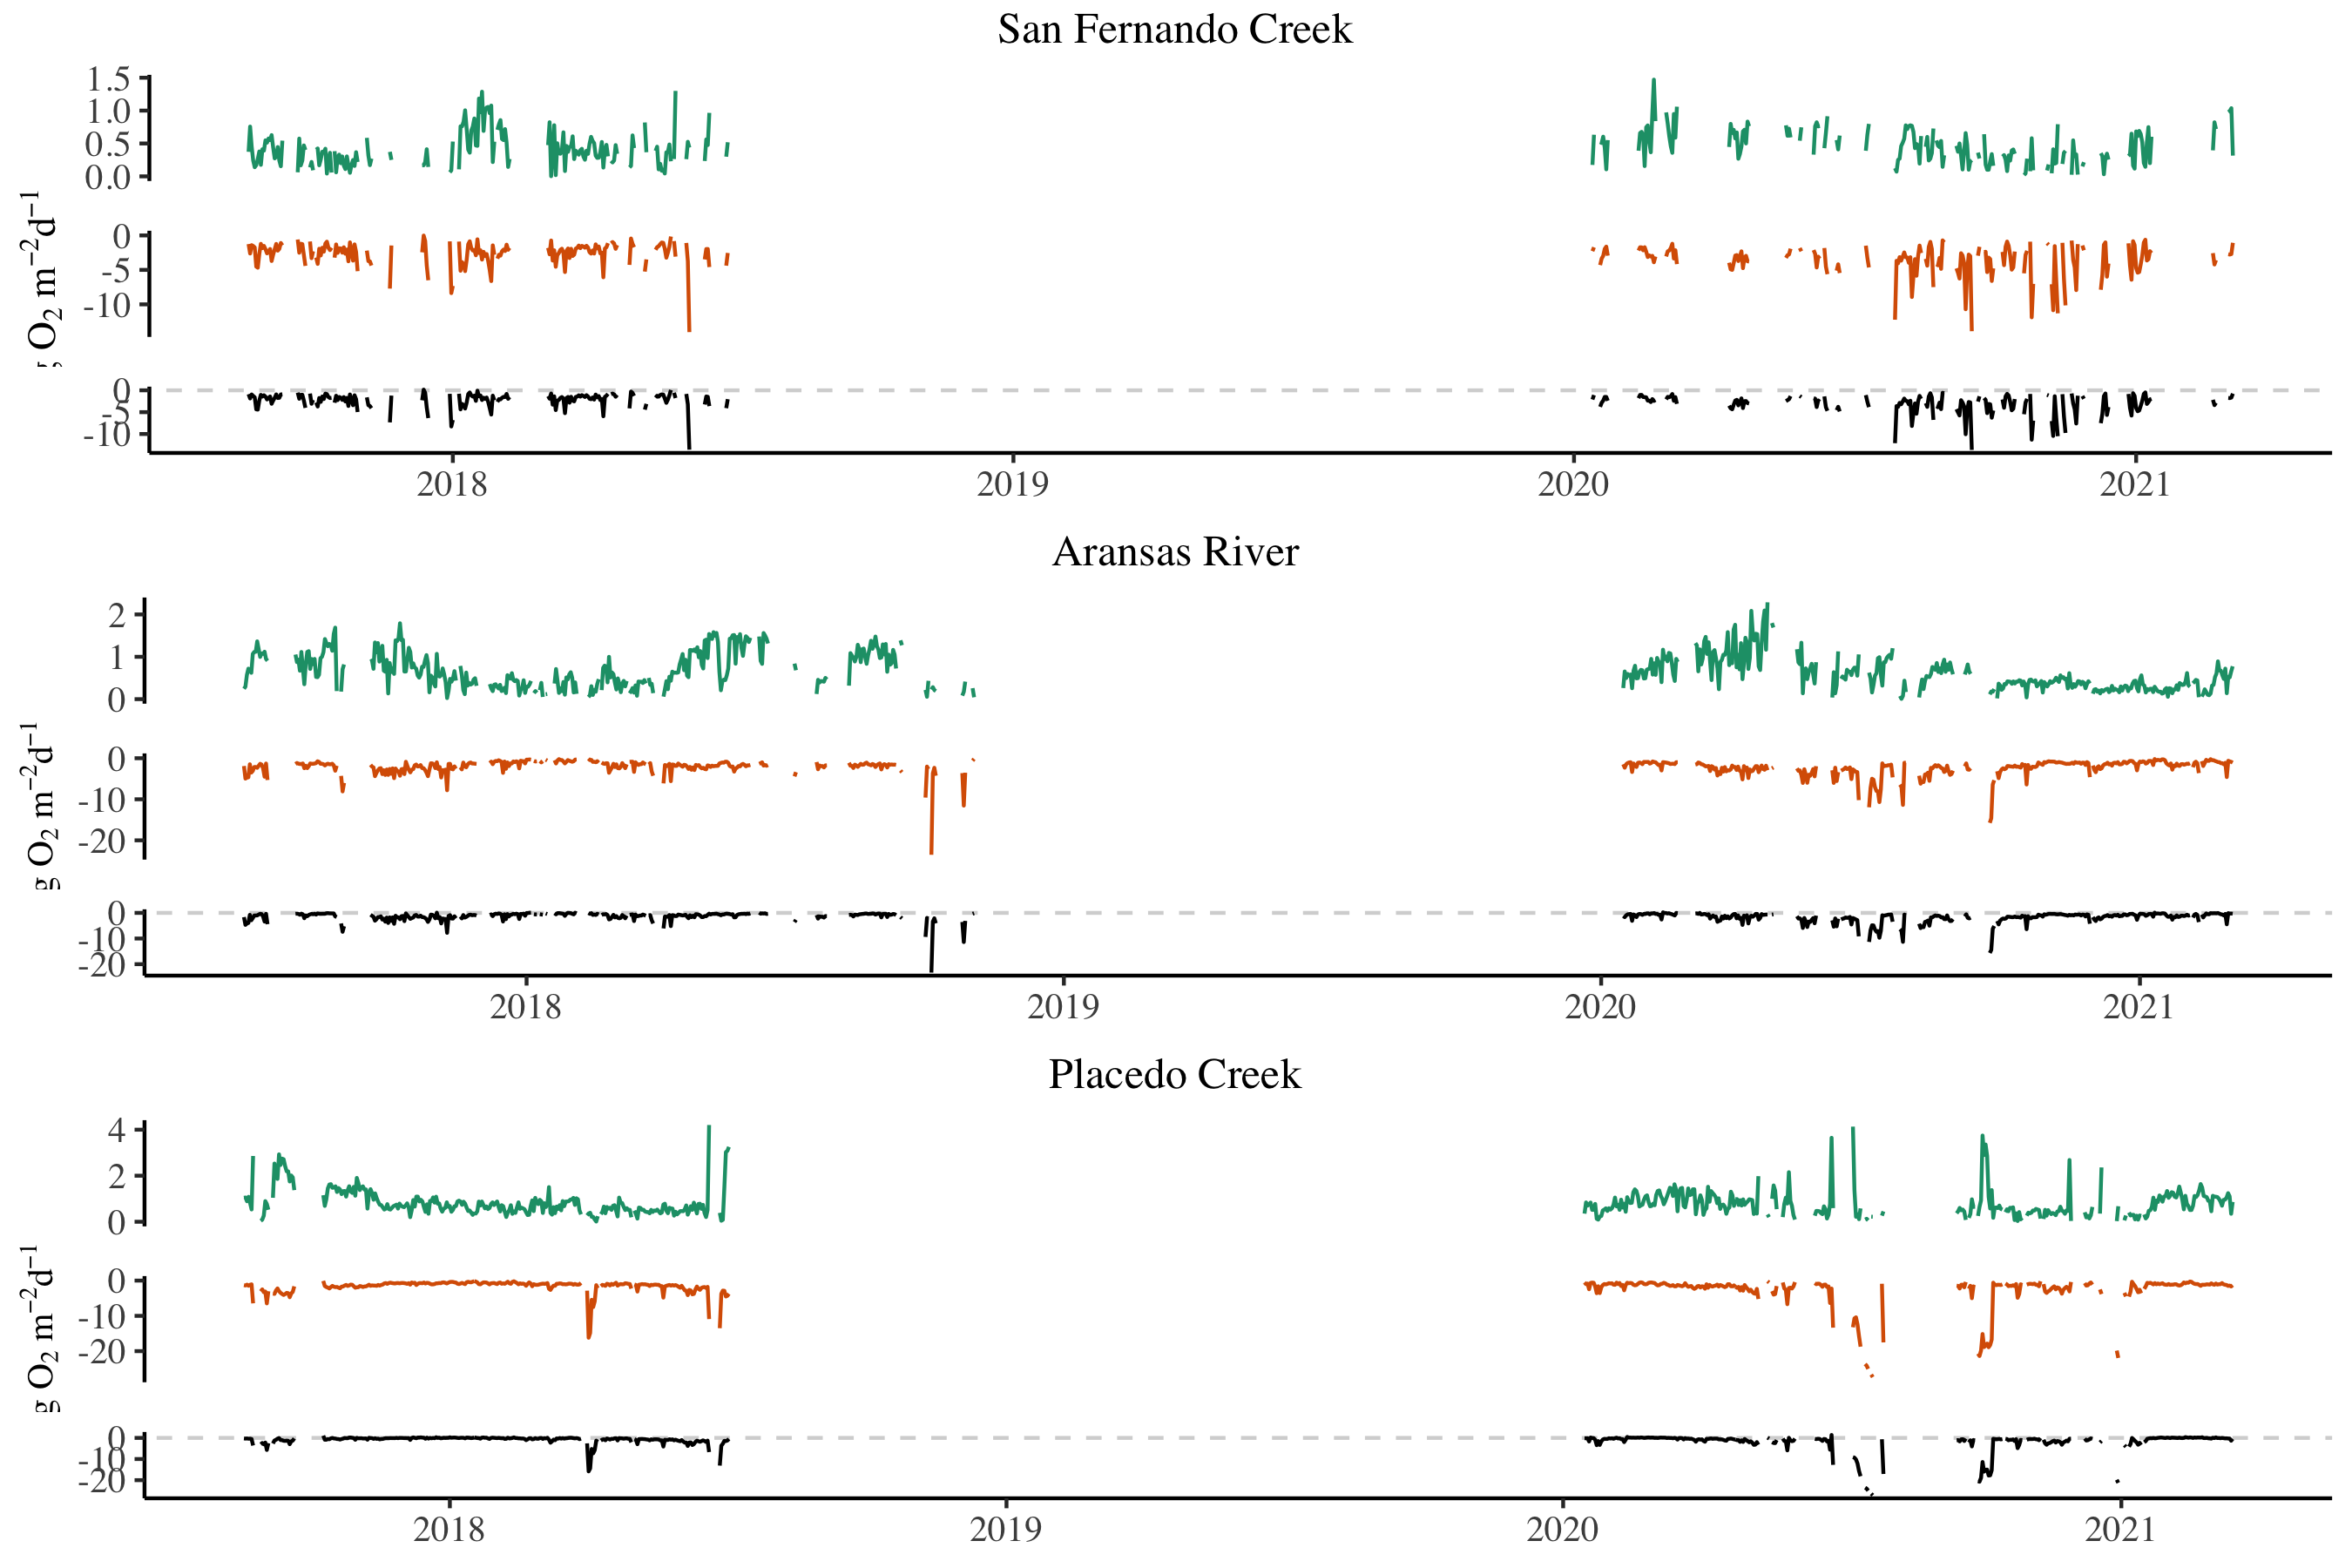
\includegraphics[scale=0.2]{Figs/MetabStacked.png}
\caption[Ecosystem Metabolism for Three Sites]{\textit{Ecosystem Metabolism for Three Sites}. Sites are arranged arid to mesic top down. Daily gross primary production (GPP, green lines) does not appear to have a distinct seasonal pattern  from 2017-2018. In comparison, during 2020, GPP appeared to vary seasonally across the sites shown here. GPP appears to increase later into the summer along the precipitation gradient, from arid to mesic. Ecosystem respiration (ER, orange lines) has the same pattern but appears to lag behind GPP. Daily net ecosystem production (NEP, black line) mirrors ER.}
\label{Fig:MetabStacked}
\end{center}
\end{figure}
\end{landscape}

\begin{landscape}
\begin{table}[htb]
\caption[Metabolism Summary]{\textit{Metabolism Summary}}\label{Tab:GPPandER}
\begin{center}
\begin{tabular}{cccccccc}
\hline\noalign{\smallskip}
Site & Usable Days & \makecell {Median GPP \\(\unit{\goxy})} & GPP 95\% CI & \makecell {Median ER \\(\unit{\goxy})} & ER 95\% CI & \makecell {Median NEP \\(\unit{\goxy})} & NEP 95\% CI\\\hline
TRC & 185 & 0.12 & 0.09-0.14 & -1.80 & -1.16 - -2.10 & -1.50 &-1.30- -1.70 \\ \
SFC & 365 & 0.39 & 0.37-0.43 & -2.60 & -2.40- -2.80 & -2.00 & -1.90- -2.20\\ 
AR & 686 & 0.54 & 0.49-0.58 & -1.70 & -1.60- -1.80 & -0.98 & -0.89- -1.10\\ 
PDC & 279 & 0.32 & 0.27-0.37 & -0.84 & -0.73- -0.93 & -0.35 & -0.30- -0.42\\ 
MR & 382 & 0.57 & 0.53-0.63 & -2.90 & --2.70- -3.10 & -2.30 & -2.00- -2.60\\ 
PLC & 609 & 0.67 & 0.63-0.71 & -1.20 & -1.20 - -1.30 & -0.46 & -0.39- -0.53\\ 
GC & 233 & 0.25 & 0.21-0.28 & -1.40 & -1.30 - -1.60 & -1.10 &  -0.97- -1.30\\ 
WMC & 263 & 0.67 & 0.62-0.79 & -11.00 & -10.00 - -12.00 & -10.00 & -9.40- -11.00\\ 
EMC & 352 & 0.78 & 0.72-0.83 & -3.30 & -3.00 - -3.60 & -2.10 & -1.80- -2.50 \\ 
\noalign{\smallskip}\hline
\end{tabular}
\end{center}
\small \textit{Note}: Number of days where I was able to estimate ecosystem metabolism, median gross primary production estimates, median ecosystem respiration estimates, and median net ecosystem production of the nine sites. CI, confidence intervals. Sites are arranged from arid to mesic top down.
\label{tab:GPP-ER}
\end{table}
\end{landscape}


\section{DOC and Nutrients}

Across all sites, average DOC ranged from 5.3 to 12.5 \unit{\mg\per\L} (Figure~\ref{Fig:DOC}). Along the precipitation gradient from semi-arid SFC to semi-mesic GC, average DOC increased (from 6.4 to 9.3 \unit{\mg\per\L}); however, average DOC concentrations at EMC, where land use is predominantly agriculture, were 5.5 \unit{\mg\per\L}, and did not follow the pattern of increasing DOC concentrations along the precipitation gradient (Figure~\ref{Fig:DOC}). Similarly, DOC concentrations at TRC, the driest site with the most non-agricultural vegetation, was the highest along the gradient (12.5 \unit{\mg\per\L}) (Table \ref{tab: Nutrients}).

Unlike DOC concentrations, there were no discernible patterns in nutrients across the precipitation gradient. Two of the sites (SFC and AR) had high levels of NO$_3$-N and PO$_4$-P, 20-185x higher for NO$_3$-N and 10-35x higher for PO$_4$-P (Figure \ref{Fig:Nitrate}~and~\ref{Fig:SPR}). Both of these sites receive waste water treatment plant effluent.

\begin{figure}[htb]
\begin{center}
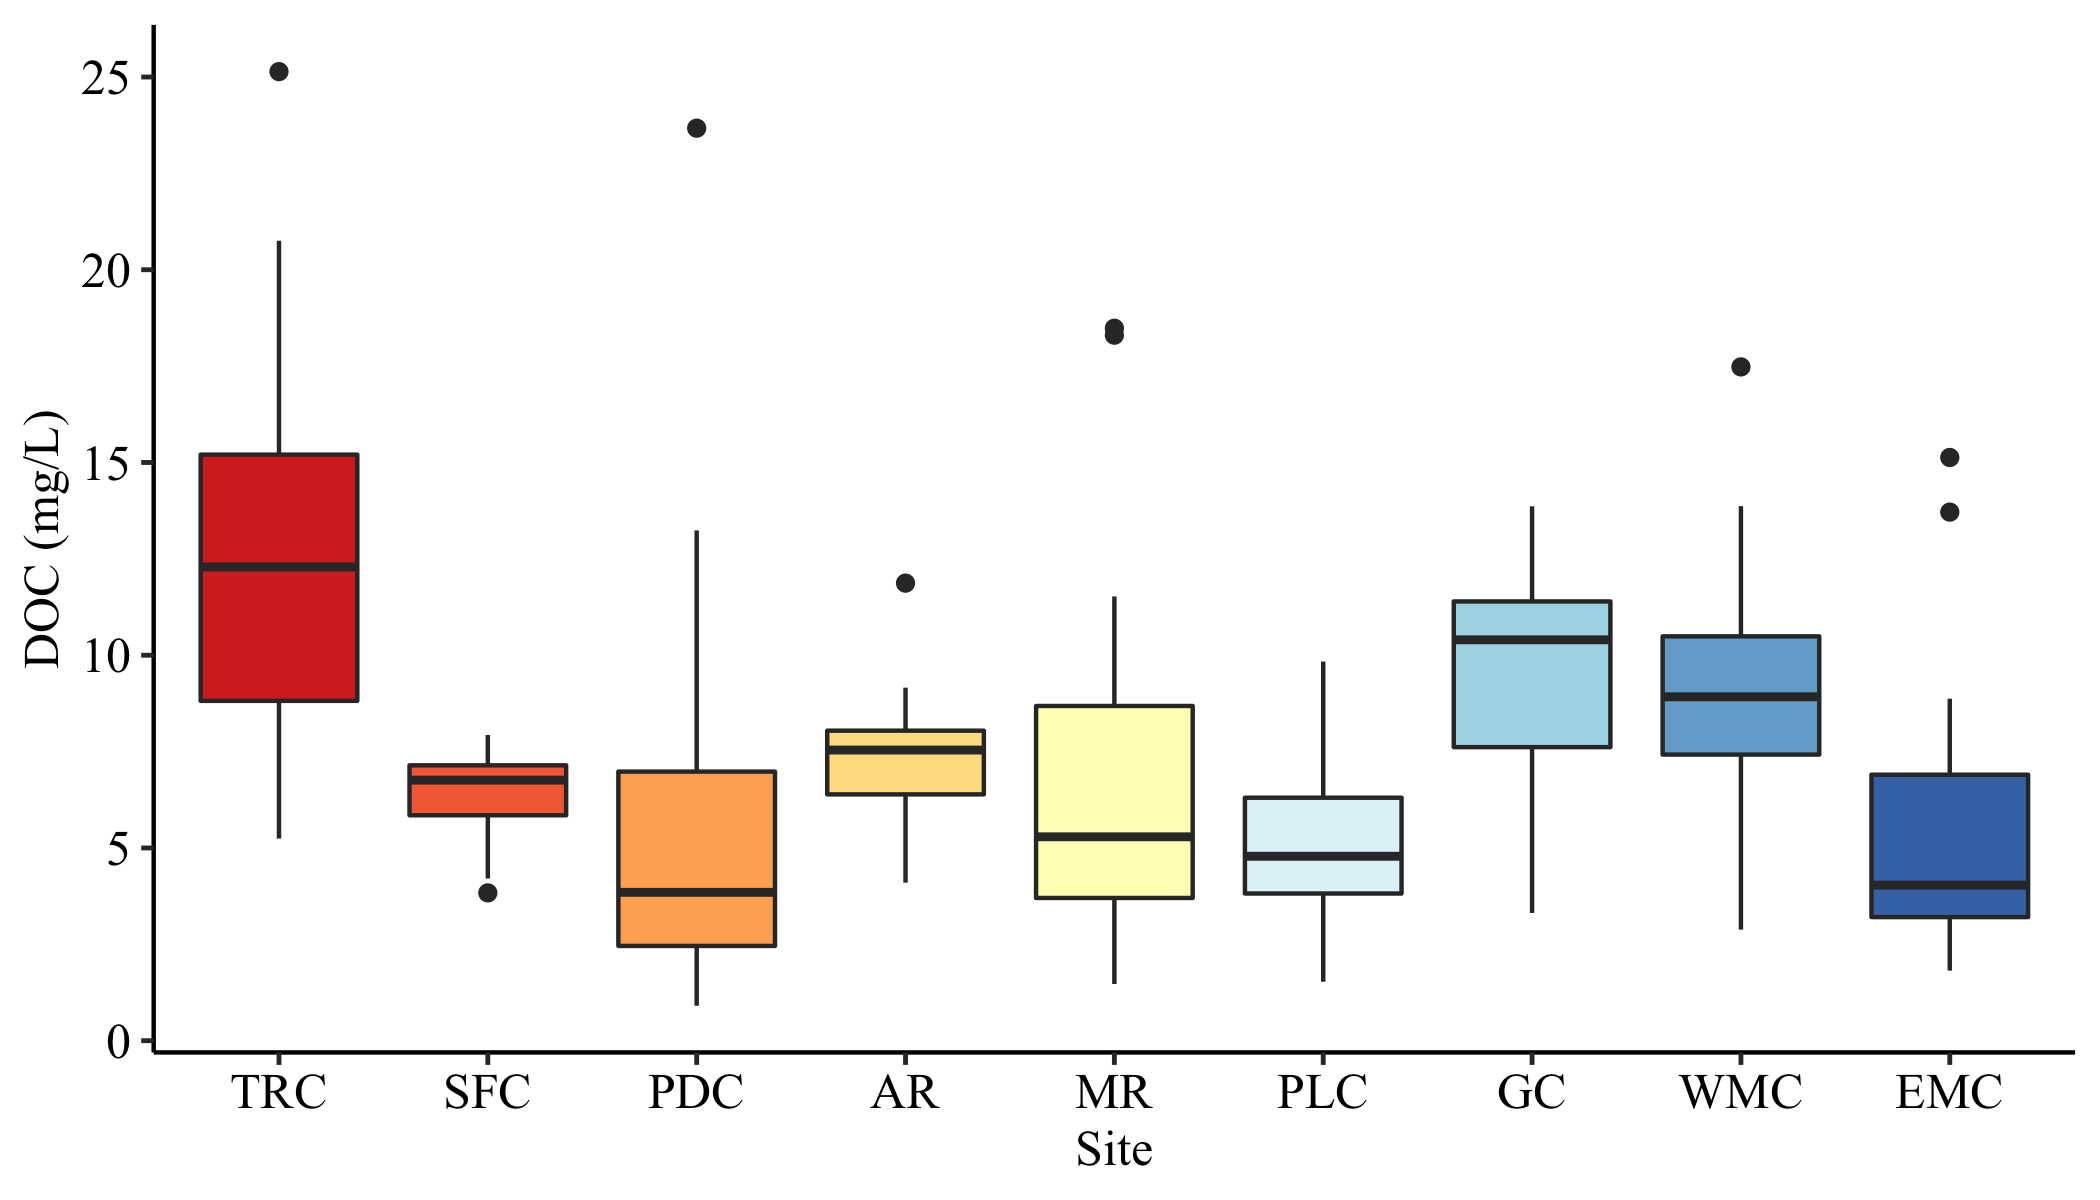
\includegraphics[scale=0.2]{Figs/DOC.png}
\caption[Dissolved Organic Carbon]{\textit{Dissolved Organic Carbon}. Sites are arranged arid to mesic left to right. Dissolved organic carbon appears to increase as precipitation increases (left to right). However, TRC and EMC do not follow this pattern. The boxes are the middle 50 quartile (25 to 75), the line is the median, the tails are 1.5X interquartile range, and any points falling outside of the line are considered outliers.
}\label{Fig:DOC}
\end{center}
\end{figure}

\begin{figure}[htb]
\begin{center}
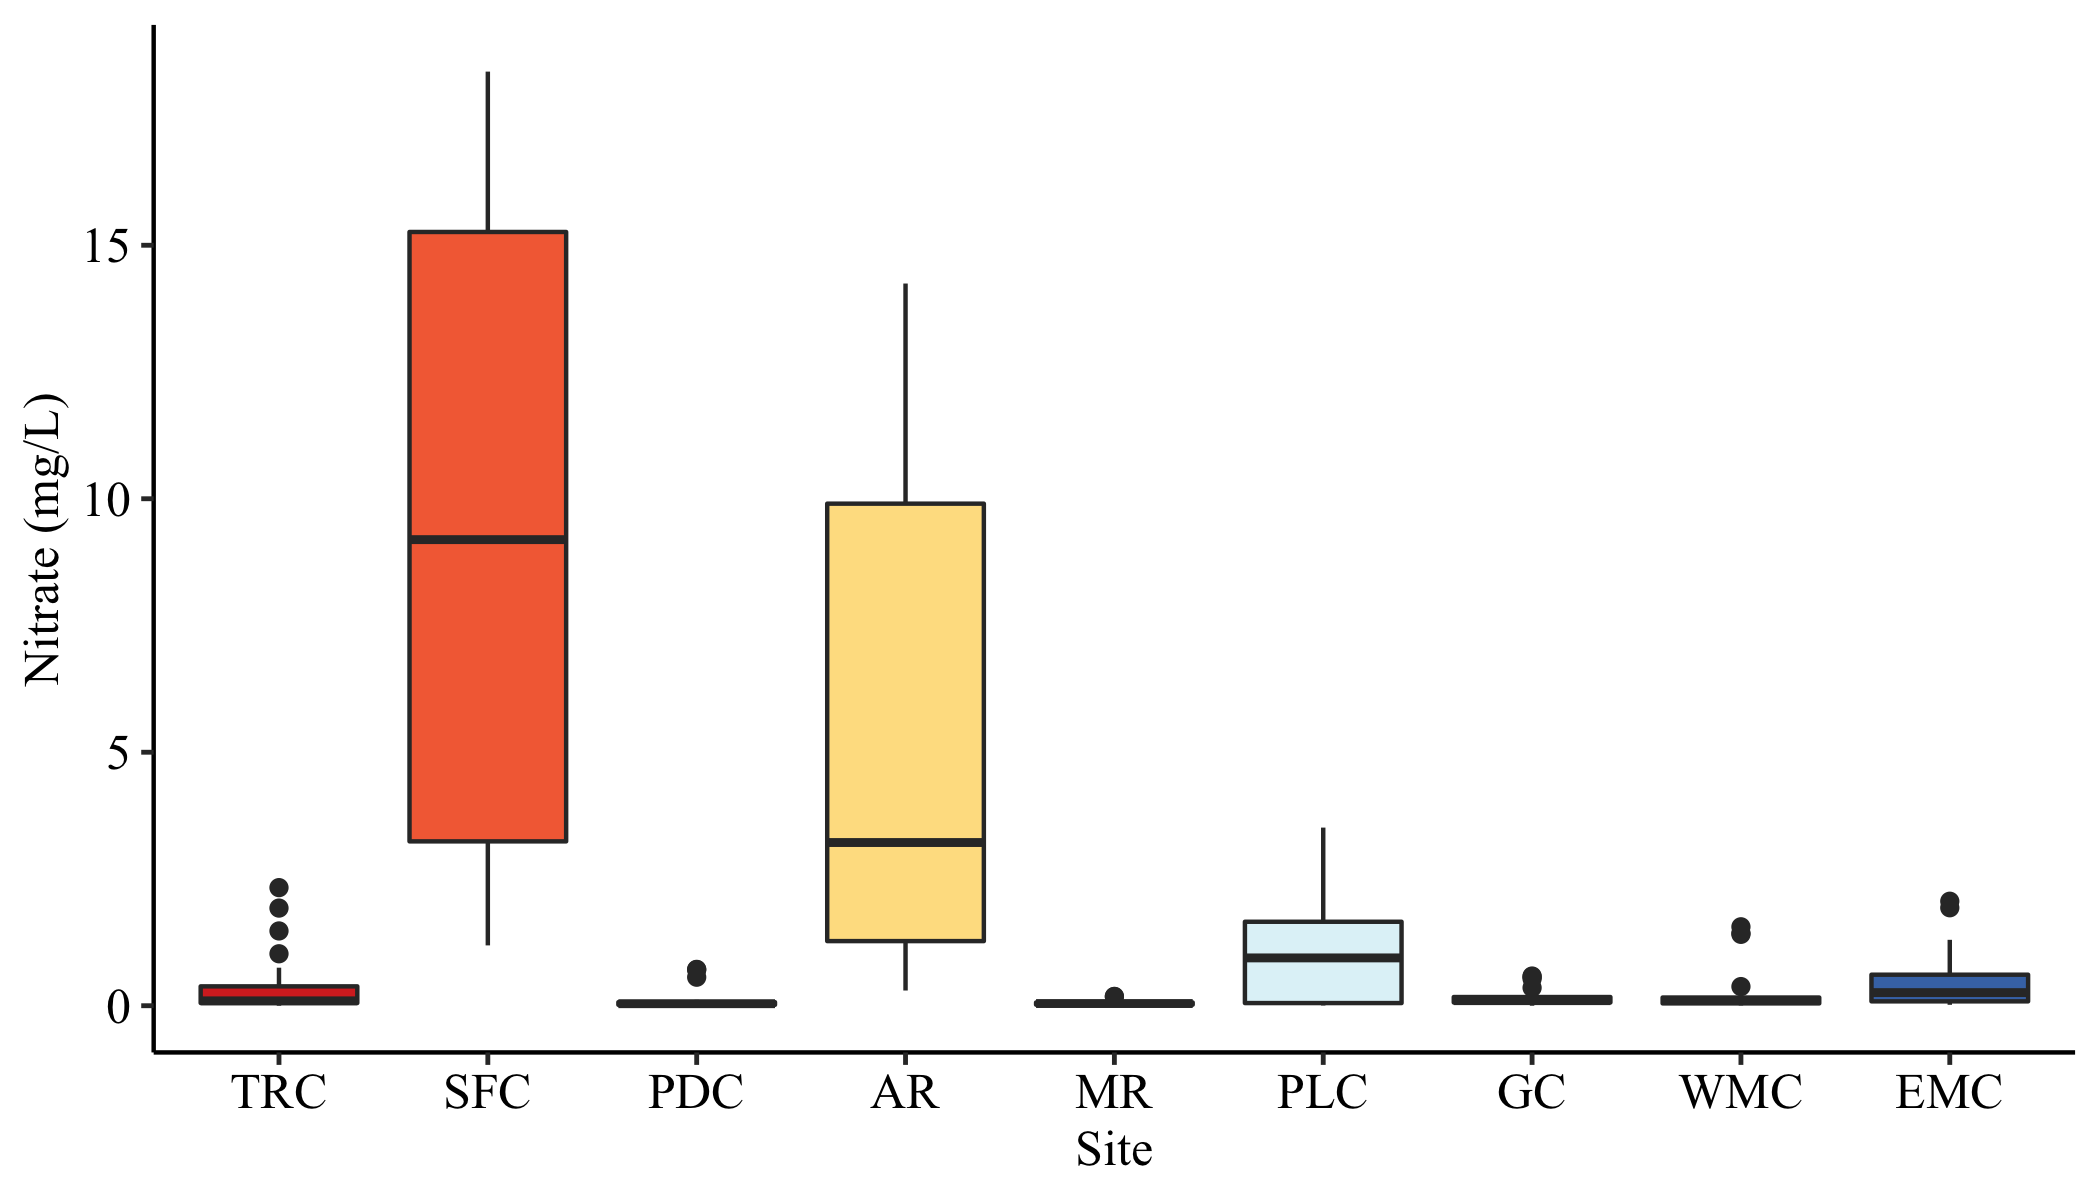
\includegraphics[scale=0.2]{Figs/NitrBox.png}
\caption[Nitrate]{\textit{Nitrate}. There does not appear to be a trend in nitrate across the precipitation gradient (Sites are arranged arid to mesic, left to right), however, SFC and AR had concentrations 20-185x higher than other study sites. The boxes are the middle 50 quartile (25 to 75), the line is the median, the tails are 1.5X interquartile range, and any points falling outside of the line are considered outliers.}
\label{Fig:Nitrate}
\end{center}
\end{figure}

\begin{figure}[htb]
\begin{center}
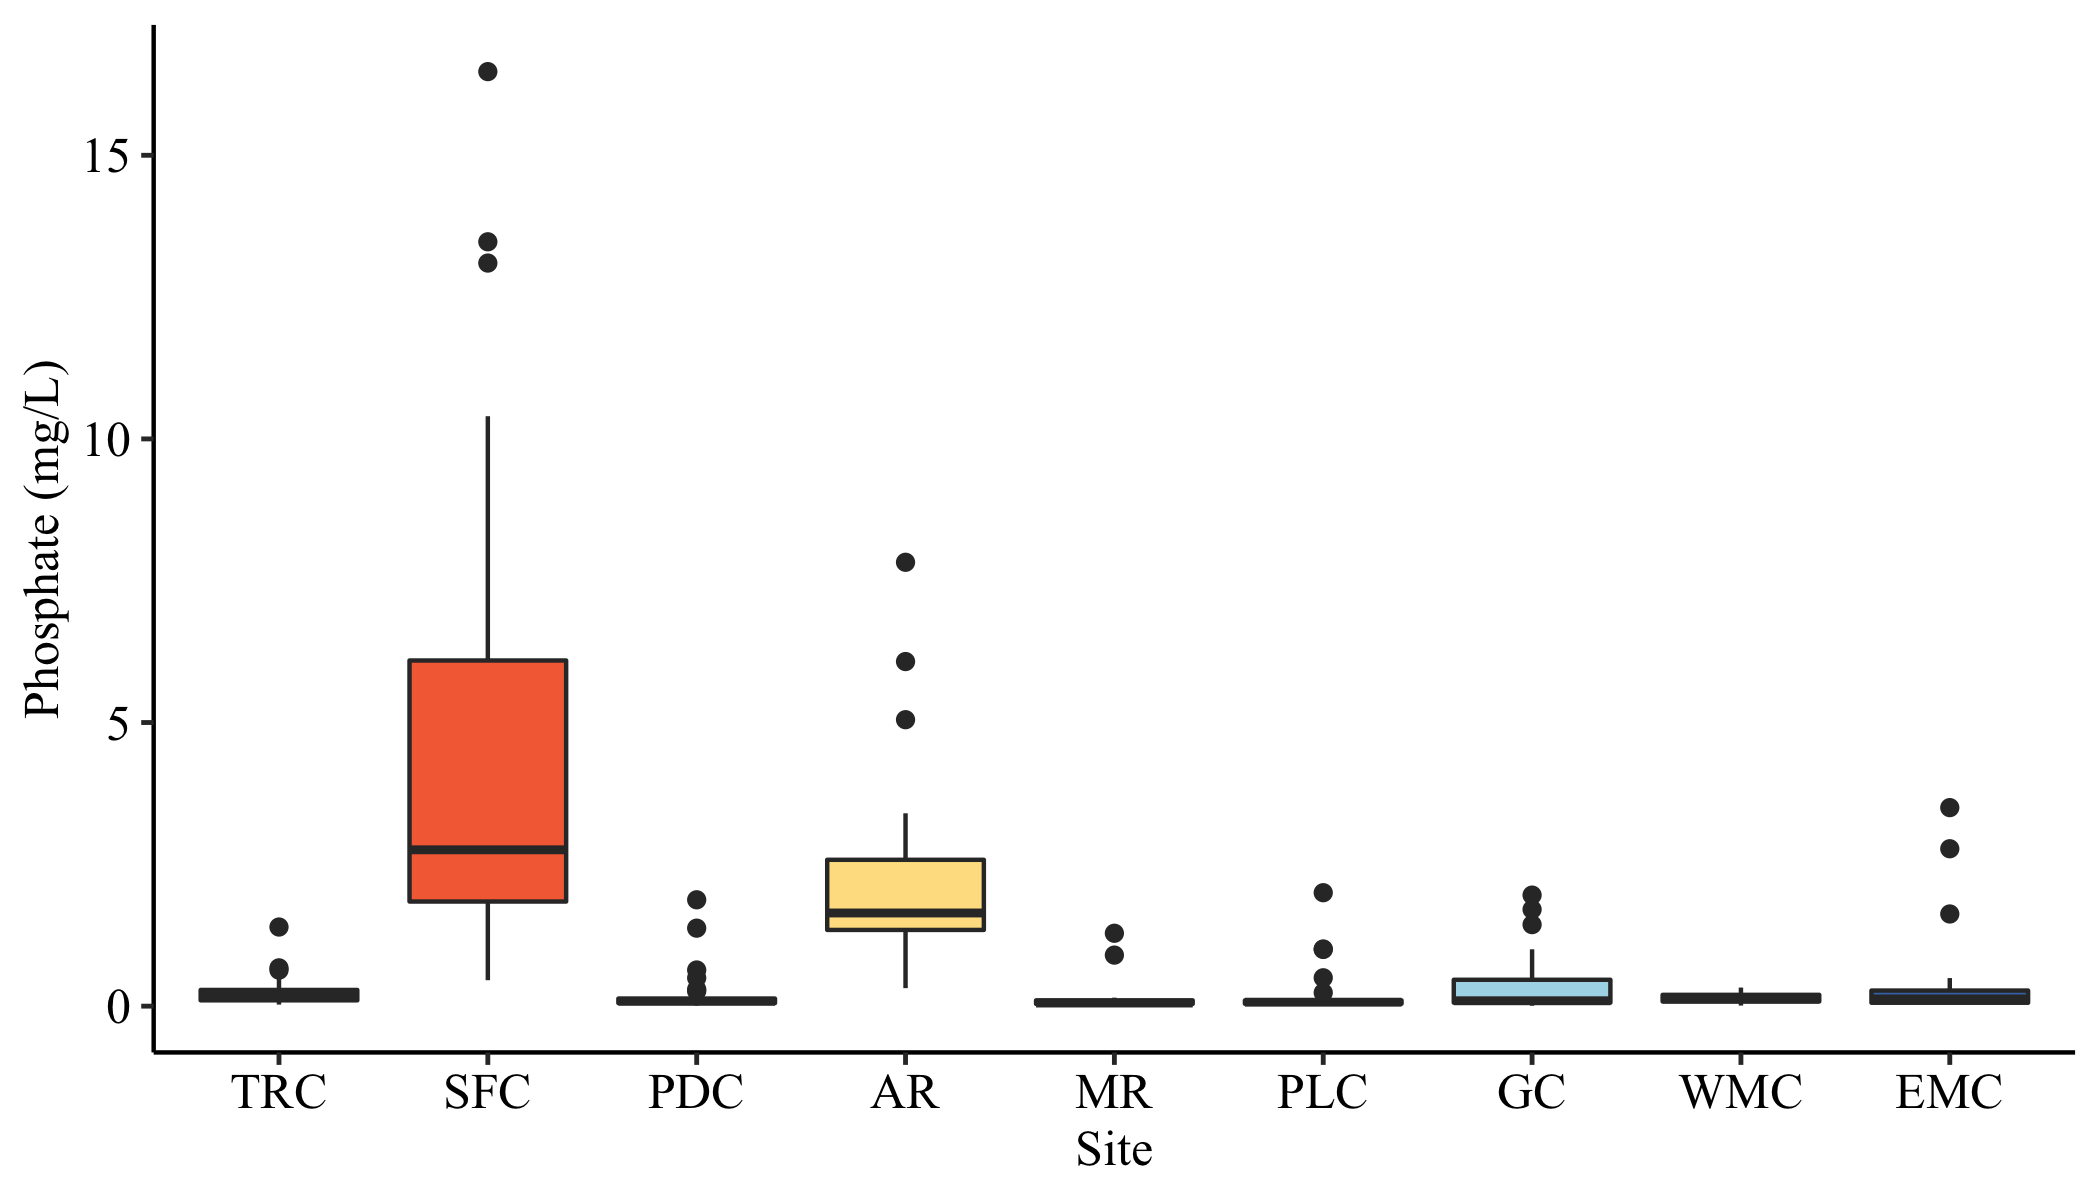
\includegraphics[scale=0.2]{Figs/OrthoPBox.png}
\caption[Soluble Reactive Phosphorous]{\textit{Soluble Reactive Phosphorous}. There does not appear to be a trend in soluble reactive phosphorous across the precipitation gradient (Sites are arranged arid to mesic, left to right), however, SFC and AR had concentrations 10-35x higher than other study sites. The boxes are the middle 50 quartile (25 to 75), the line is the median, the tails are 1.5X interquartile range, and any points falling outside of the line are considered outliers.}
\label{Fig:SPR}
\end{center}
\end{figure}

\begin{table}[htb]
\caption[DOC and Nutrient Concentrations]{\textit{DOC and Nutrient Concentrations}}
\begin{center}
\begin{tabular}
[c]{ccccc}\hline
Site & \makecell {DOC $\pm$ SD\\(\unit{\mg\per\L})} & \makecell {NH$_4$-N $\pm$ SD\\(\unit{\mg\per\L})} & \makecell {NO$_3$-N $\pm$ SD\\(\unit{\mg\per\L})} & \makecell {PO$_4$-P $\pm$ SD\\(\unit{\mg\per\L})}\\\hline
TRC & 12.5 $\pm$ 4.8 & 0.22 $\pm$ 0.16 & 0.39 $\pm$ 0.61 & 0.27 $\pm$ 0.28\\
SFC & 6.4 $\pm$ 1.16 & 0.18 $\pm$ 0.01 & 9.25 $\pm$ 6.0 & 4.60 $\pm$ 4.40\\
AR & 7.2 $\pm$ 1.80 &0.16 $\pm$ 0.14 & 5.1 $\pm$ 4.50 & 2.22 $\pm$ 1.70\\
PDC & 5.8 $\pm$ 5.40 & 0.14 $\pm$ 0.01 & 0.11 $\pm$ 0.20 & 0.23 $\pm$ 0.42\\
MR & 6.9 $\pm$ 4.70 & 0.13 $\pm$ 0.10 & 0.05 $\pm$ 0.05 & 0.13 $\pm$ 0.30\\
PLC	 & 5.3 $\pm$ 2.40 & 0.13 $\pm$ 0.05 & 1.06 $\pm$ 1.21 & 0.23 $\pm$ 0.44\\
GC & 9.3 $\pm$ 3.15 & 0.18 $\pm$ 0.22 & 0.16 $\pm$ 0.16 & 0.39 $\pm$ 0.56\\
WMC & 9.1 $\pm$ 3.20 & 0.13 $\pm$ 0.063 & 0.26 $\pm$ 0.45 & 0.14 $\pm$ 0.08\\
EMC & 5.5 $\pm$ 3.55 & 0.13 $\pm$ 0.07 & 0.45 $\pm$ 0.54 & 0.42 $\pm$ 0.83\\\hline
\end{tabular}
\end{center}
\textit{Note}: Average concentrations of dissolved organic carbon (DOC), ammonium (NH$_4$-N), nitrate (NO$_3$-N), and phosphate (PO$_4$-P) across the precipitation gradient (sites are arranged arid to mesic, top down). San Fernando Creek and Aransas River both receive water from waste water treatment plants. SD, standard deviation.
\label{tab: Nutrients}
\end{table}

\section{Discharge}

Across the precipitation and land use gradients, average discharged ranged from \qtyrange{.03}{3.00}{\cubic\m\per\second}, with WMC having the highest discharge, and PDC the flashiest (Table~\ref{tab:Q}). Across the gradients, discharge greatly varied between sites and had quick responses to storm events (Figure \ref{Fig:Q}).

\begin{table}
\caption[Summary of Site Discharge]{\textit{Summary of Site Discharge}}
\begin{center}
\begin{tabular}[c]{ccccc}
\hline
Site & \makecell{Mean Discharge\\(\unit{\cubic\m\per\s})} & \makecell{Median Discharge\\(\unit{\cubic\m\per\s})} & \makecell{CV\\(\%)}\\
\hline
TRC & 0.03 & 0.00 & 447.32\\
SFC & 0.19 & 0.03 & 1586.92\\
PDC & 0.12 & 0.00 & 1112.93\\
AR & 0.37 & 0.10 & 551.65\\
MR & 2.49 & 0.13 & 578.40\\
PLC & 1.17 & 0.03 & 760.08\\
GC & 0.71 & 0.01 & 909.21\\
WMC & 3.00 & 0.37 & 433.70\\
EMC & 0.90 & 0.04 & 457.34\\
\hline
\end{tabular}
\end{center}
\label{tab:Q}
\textit{Note}: Mean, median, and Coefficient of Variation (CV) of site discharge across the precipitation gradient (sites are arranged arid to mesic, top down).
\end{table}

\begin{figure}[htb]
\begin{center}
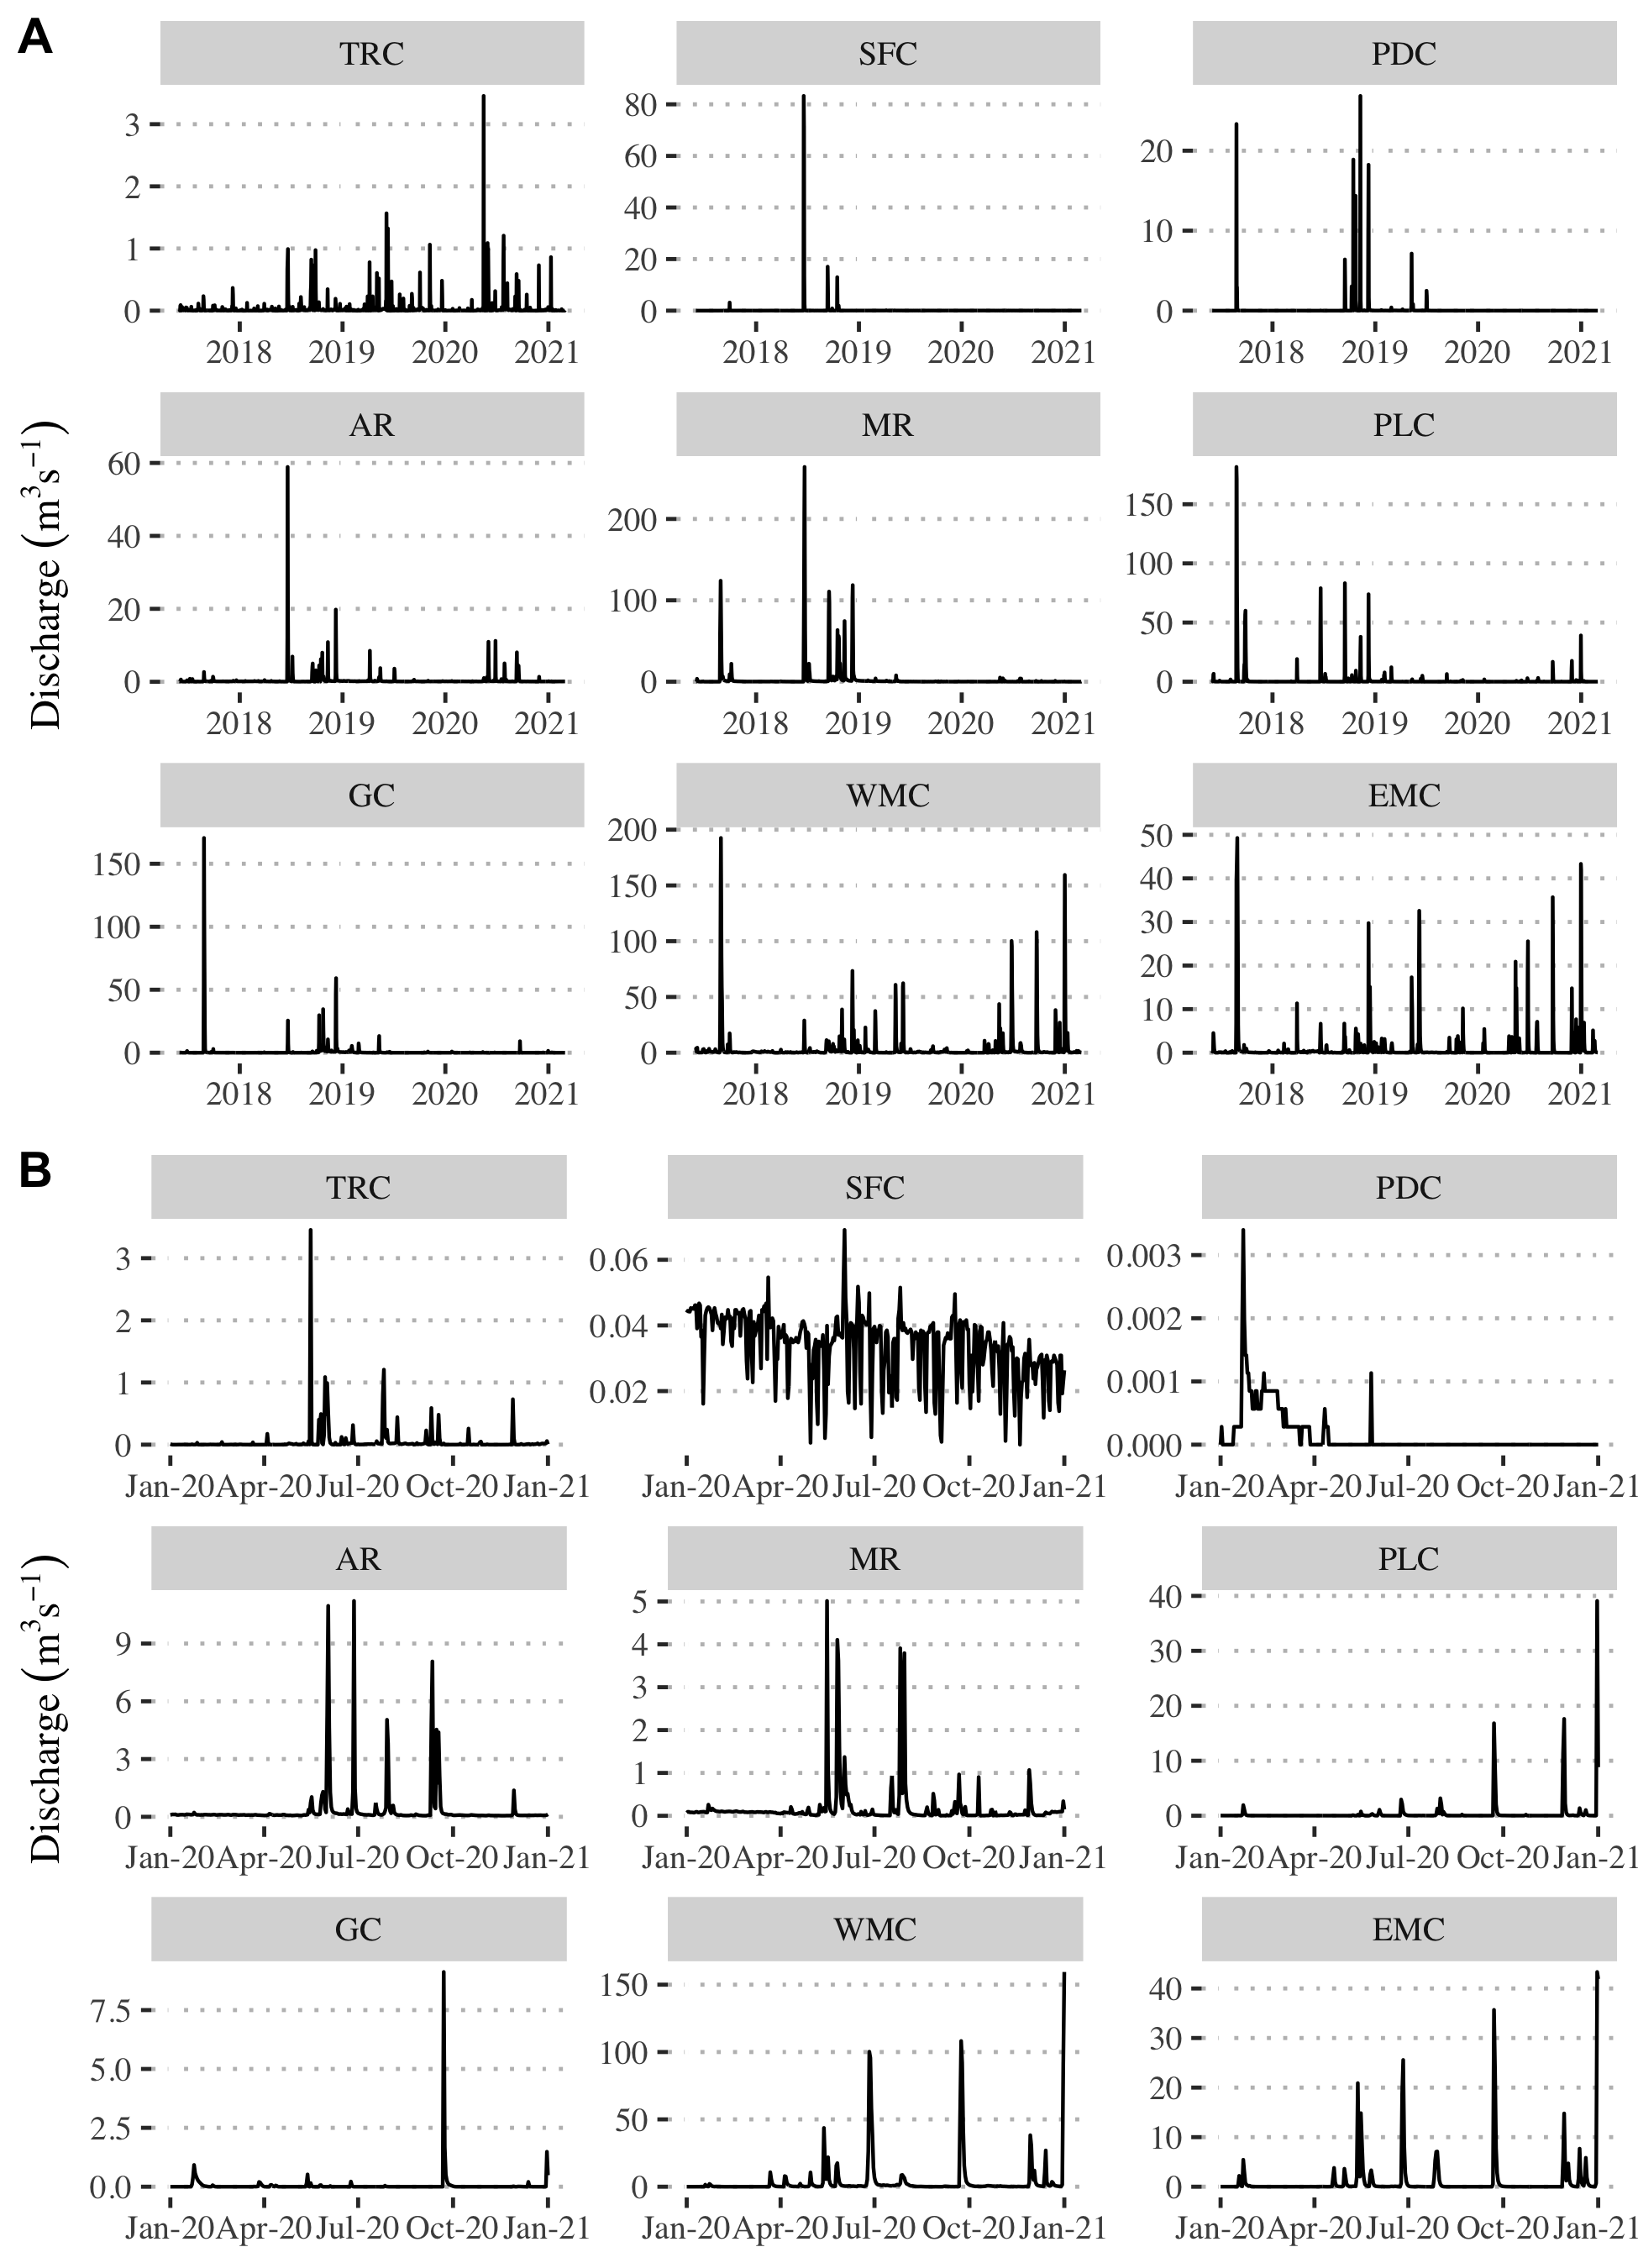
\includegraphics[scale = 0.21]{Figs/Q2020.png}
\caption[Site Discharge]{\textit{Site Discharge}. Sites are arranged arid to mesic left to right and top to bottom. Discharge appears to increase along the gradients, however they are punctuated by sharp increases due to rainfall. Note the different y-axis. Figure A is discharge over the study period, while figure B is 2020.}
\label{Fig:Q}
\end{center}
\end{figure}



\section{Principal Component Analysis and Structural Equation Model}

The PCA based on percentages of watershed land use categories identified two gradients in these sites. Land use-PC1, explaining 44.1\% of the variation, and was explained by wetlands, shrubs, and grasslands to cropland and developed land, while land use-PC2, explaining 29\% of the variation, ordered streams along a gradient of forest and pasture relative to other land uses  (Figure~\ref{Fig:PCA}). PC values were used as a proxy for watershed land use in the structural equation model to evaluate distal and proximal drivers of GPP and ER.

\begin{figure}[htb]
\begin{center}
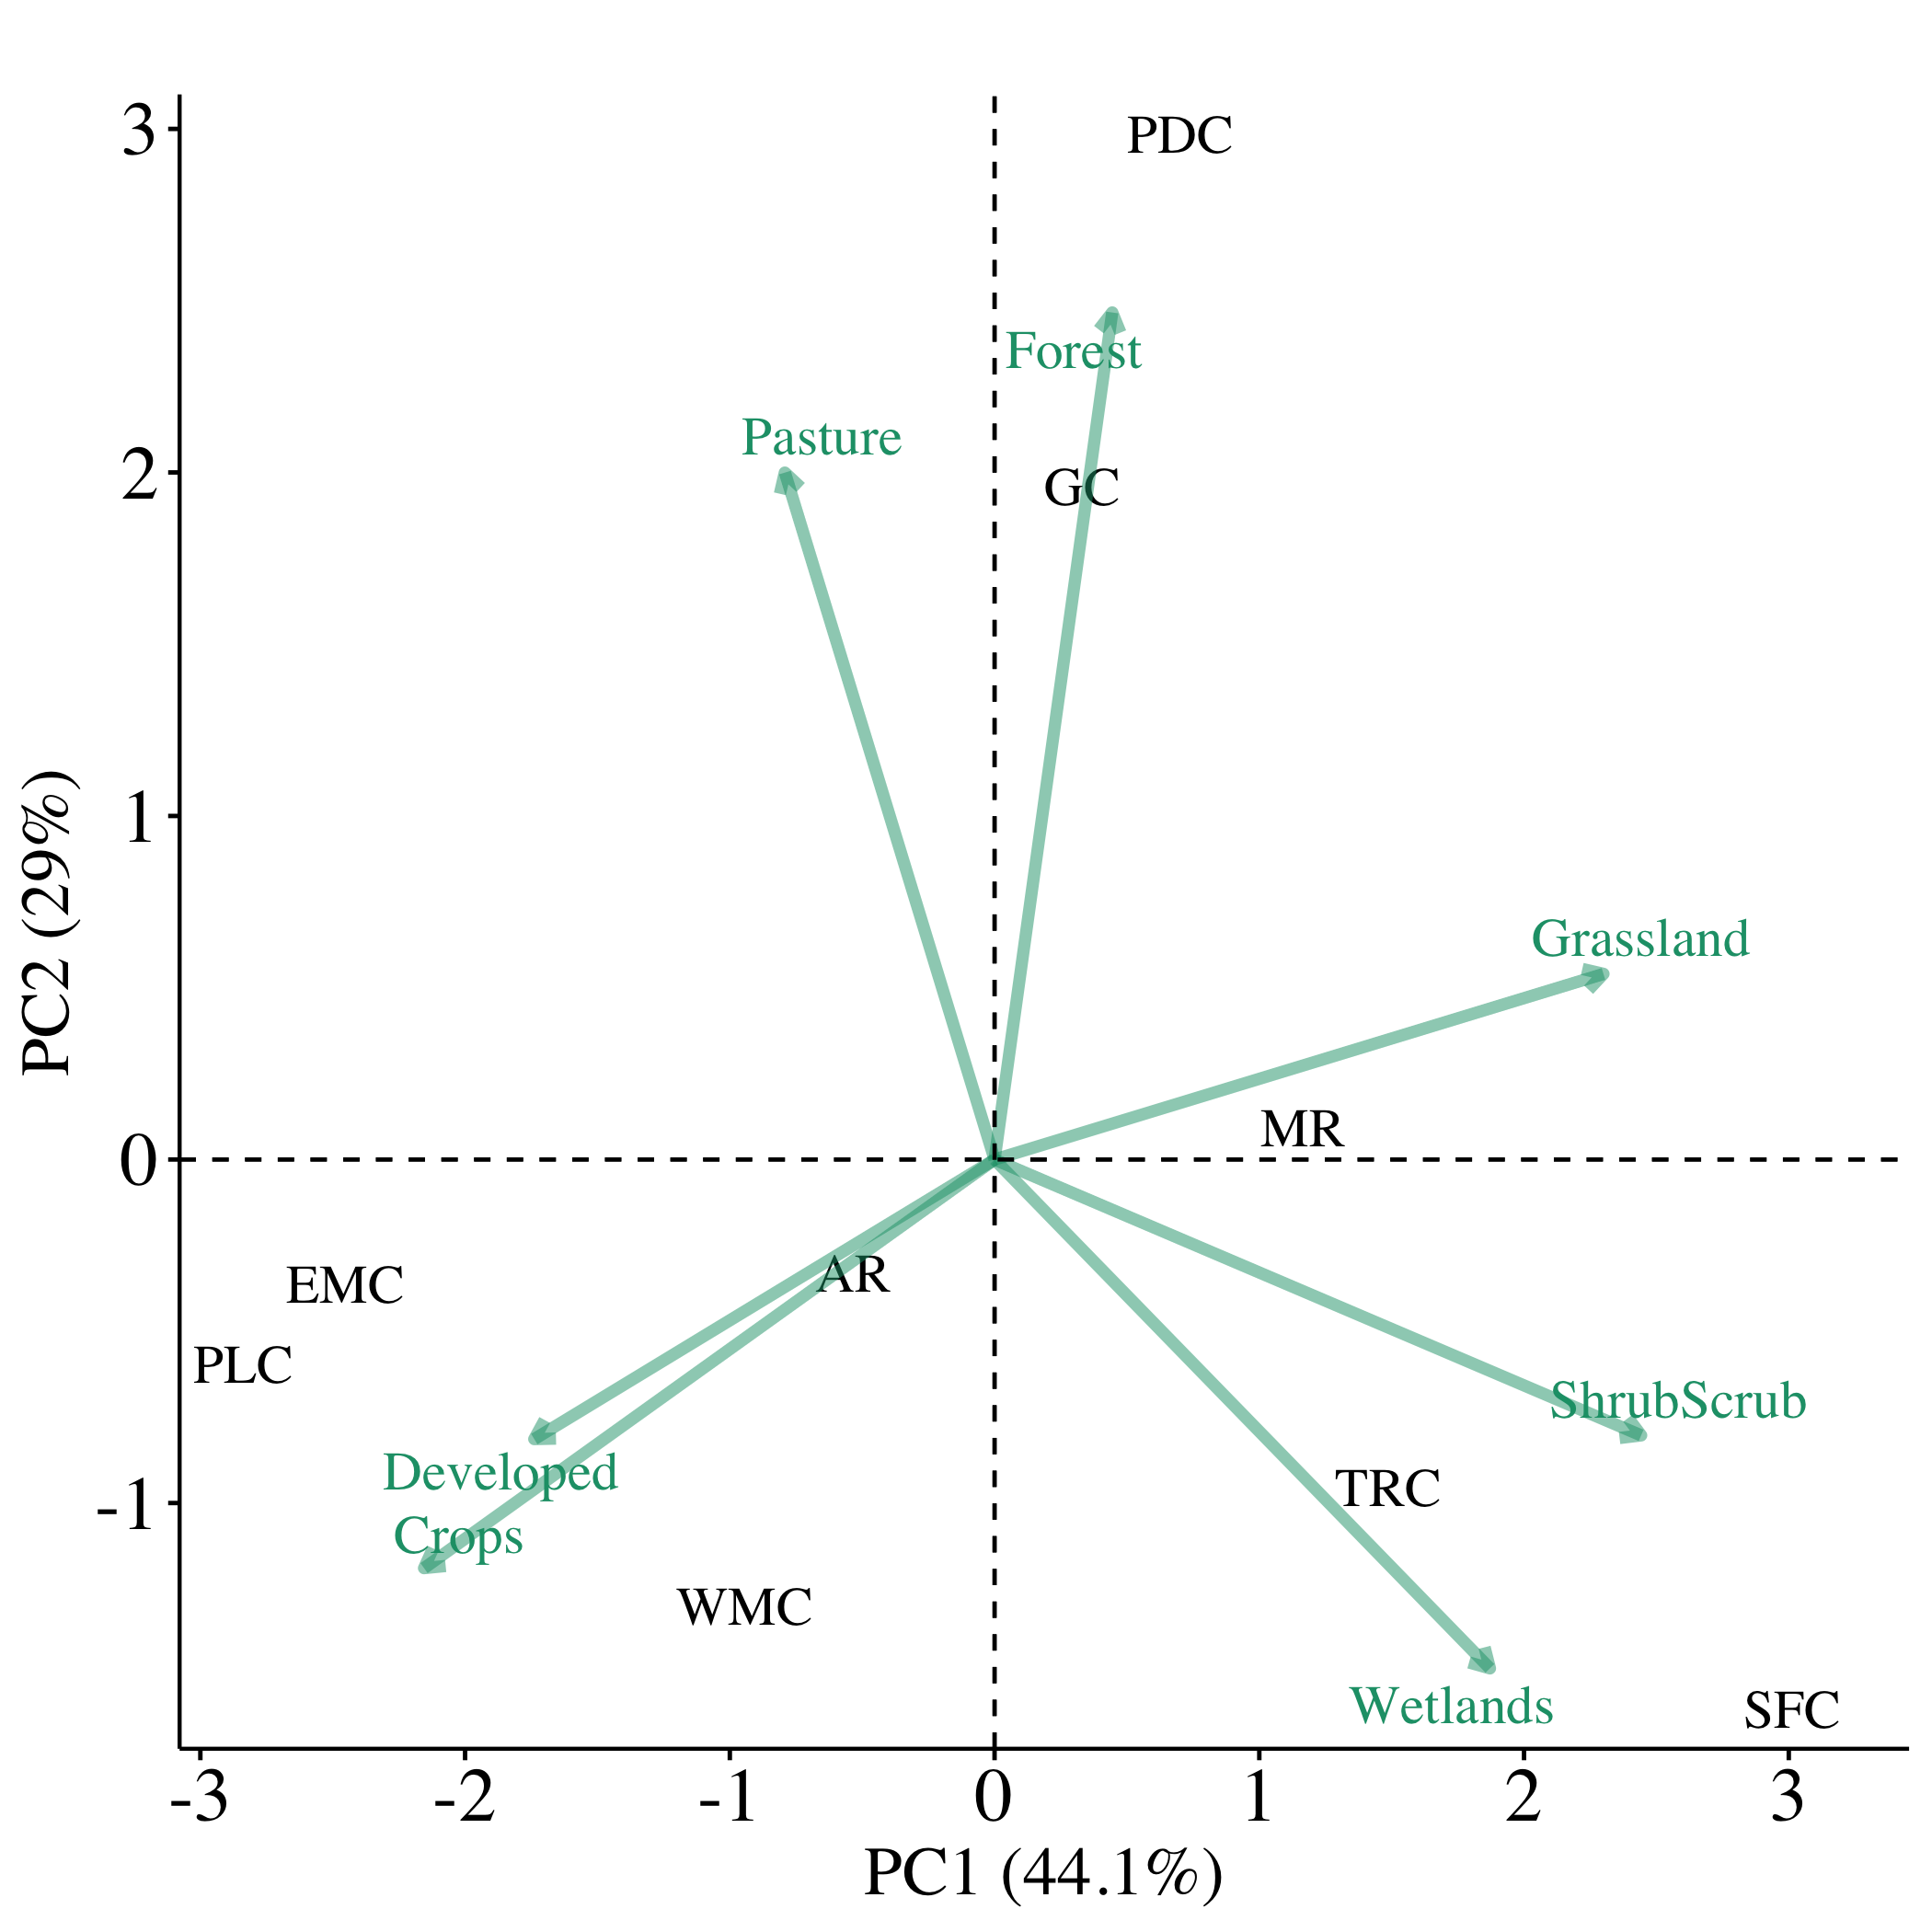
\includegraphics[scale=0.2]{Figs/PCA.png}
\caption[Principal Component Analysis]{\textit{Principal Component Analysis}. Principal component 1 ordered streams along a gradient of wetlands, shrubs, and grasslands to cropland and developed land, while principal component 2 grouped forest and pasture together.}
\label{Fig:PCA}
\end{center}
\end{figure}


I used a structural equation model to parse out the drivers of GPP and ER. I used the proximal drivers, average monthly precipitation, the presence of WWTP in the watershed, and land use PC1 and PC2 and distal drivers, discharge (CV), DOC, nitrate, and phosphate to explain the variability in monthly GPP and ER. I was unable to find a statistically significant model for the drivers of GPP and ER (Figure~\ref{Fig:SEMmetab}). However, when GPP and ER were removed from the model, there was a statistically significant model (Figure~\ref{Fig:SEMdrivers}). The results of the second SEM without GPP and ER indicated that land use PC1 and PC2 are strongly driving NO$_3$-N, PO$_4$-P, DOC, and turbidity, while monthly average precipitation is weakly driving NO$_3$-N and DOC.

\begin{landscape}
\begin{figure}[htb]
\begin{center}
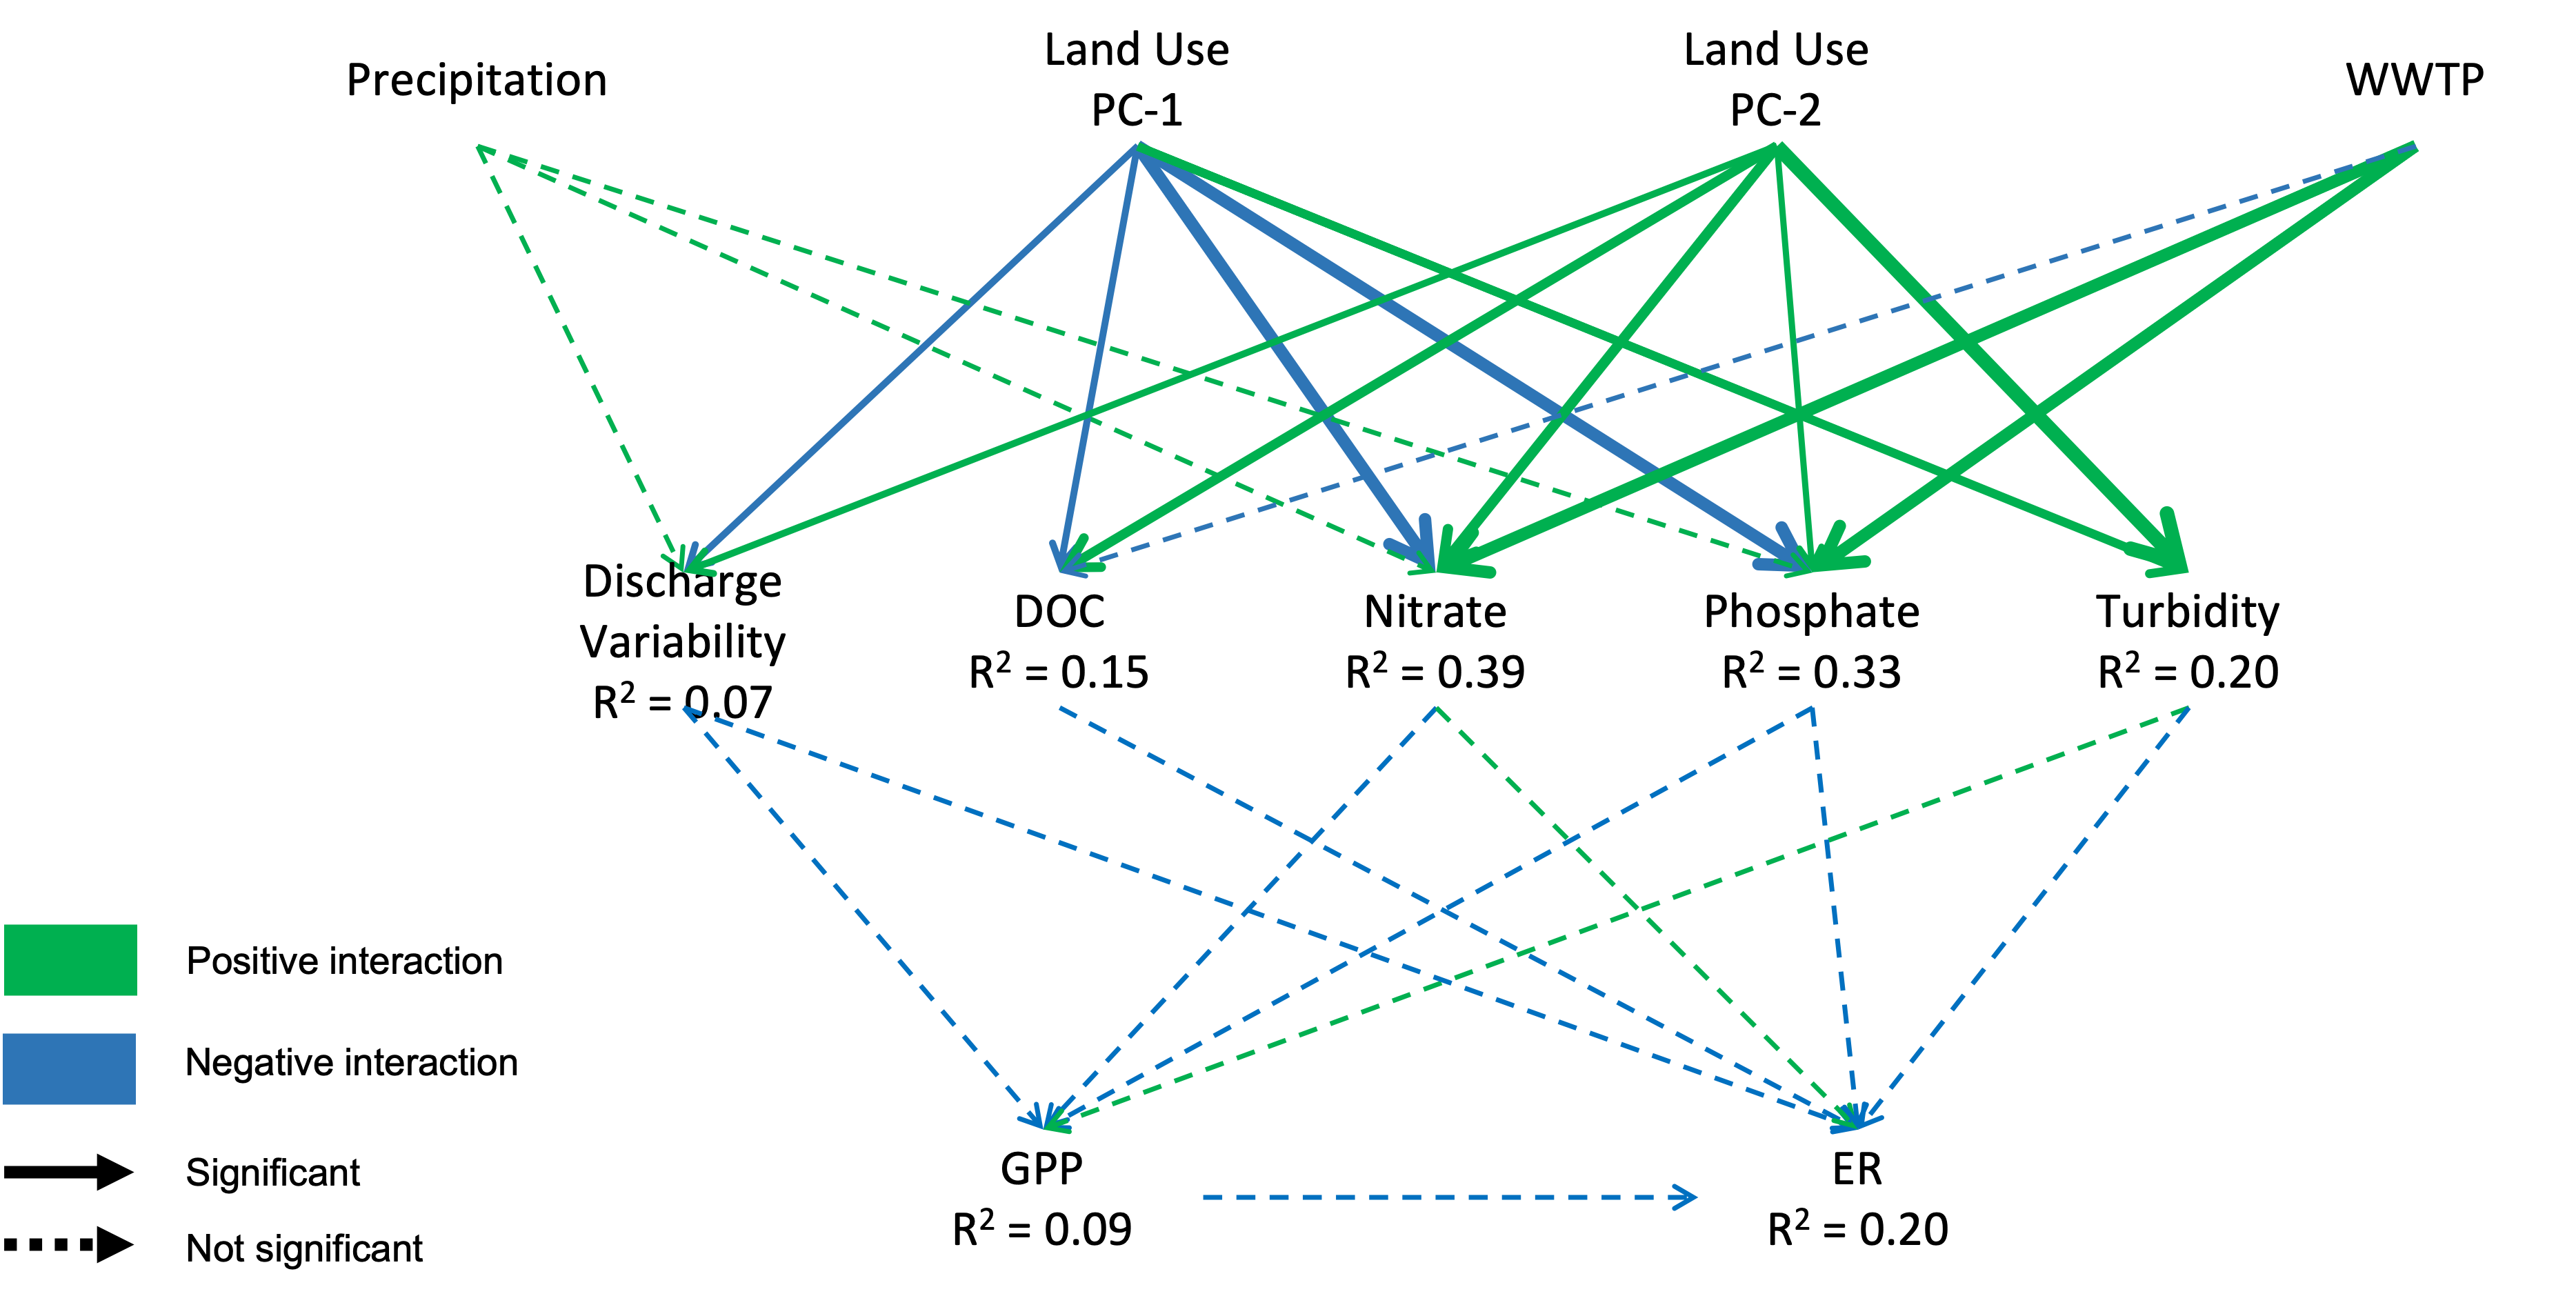
\includegraphics[scale=0.8]{Figs/SEMmetab.png}
\caption[SEM 1]{\textit{SEM 1}. The land use PCs (PC1 and PC2) and precipitation gradient had a strong impact on the proximal drivers (discharge, turbidity, DOC, nitrate, and phosphate), however, this interaction did not reach gross primary production or ecosystem respiration.}
\label{Fig:SEMmetab}
\end{center}
\end{figure}
\end{landscape}

\begin{landscape}
\begin{figure}[htb]
\begin{center}
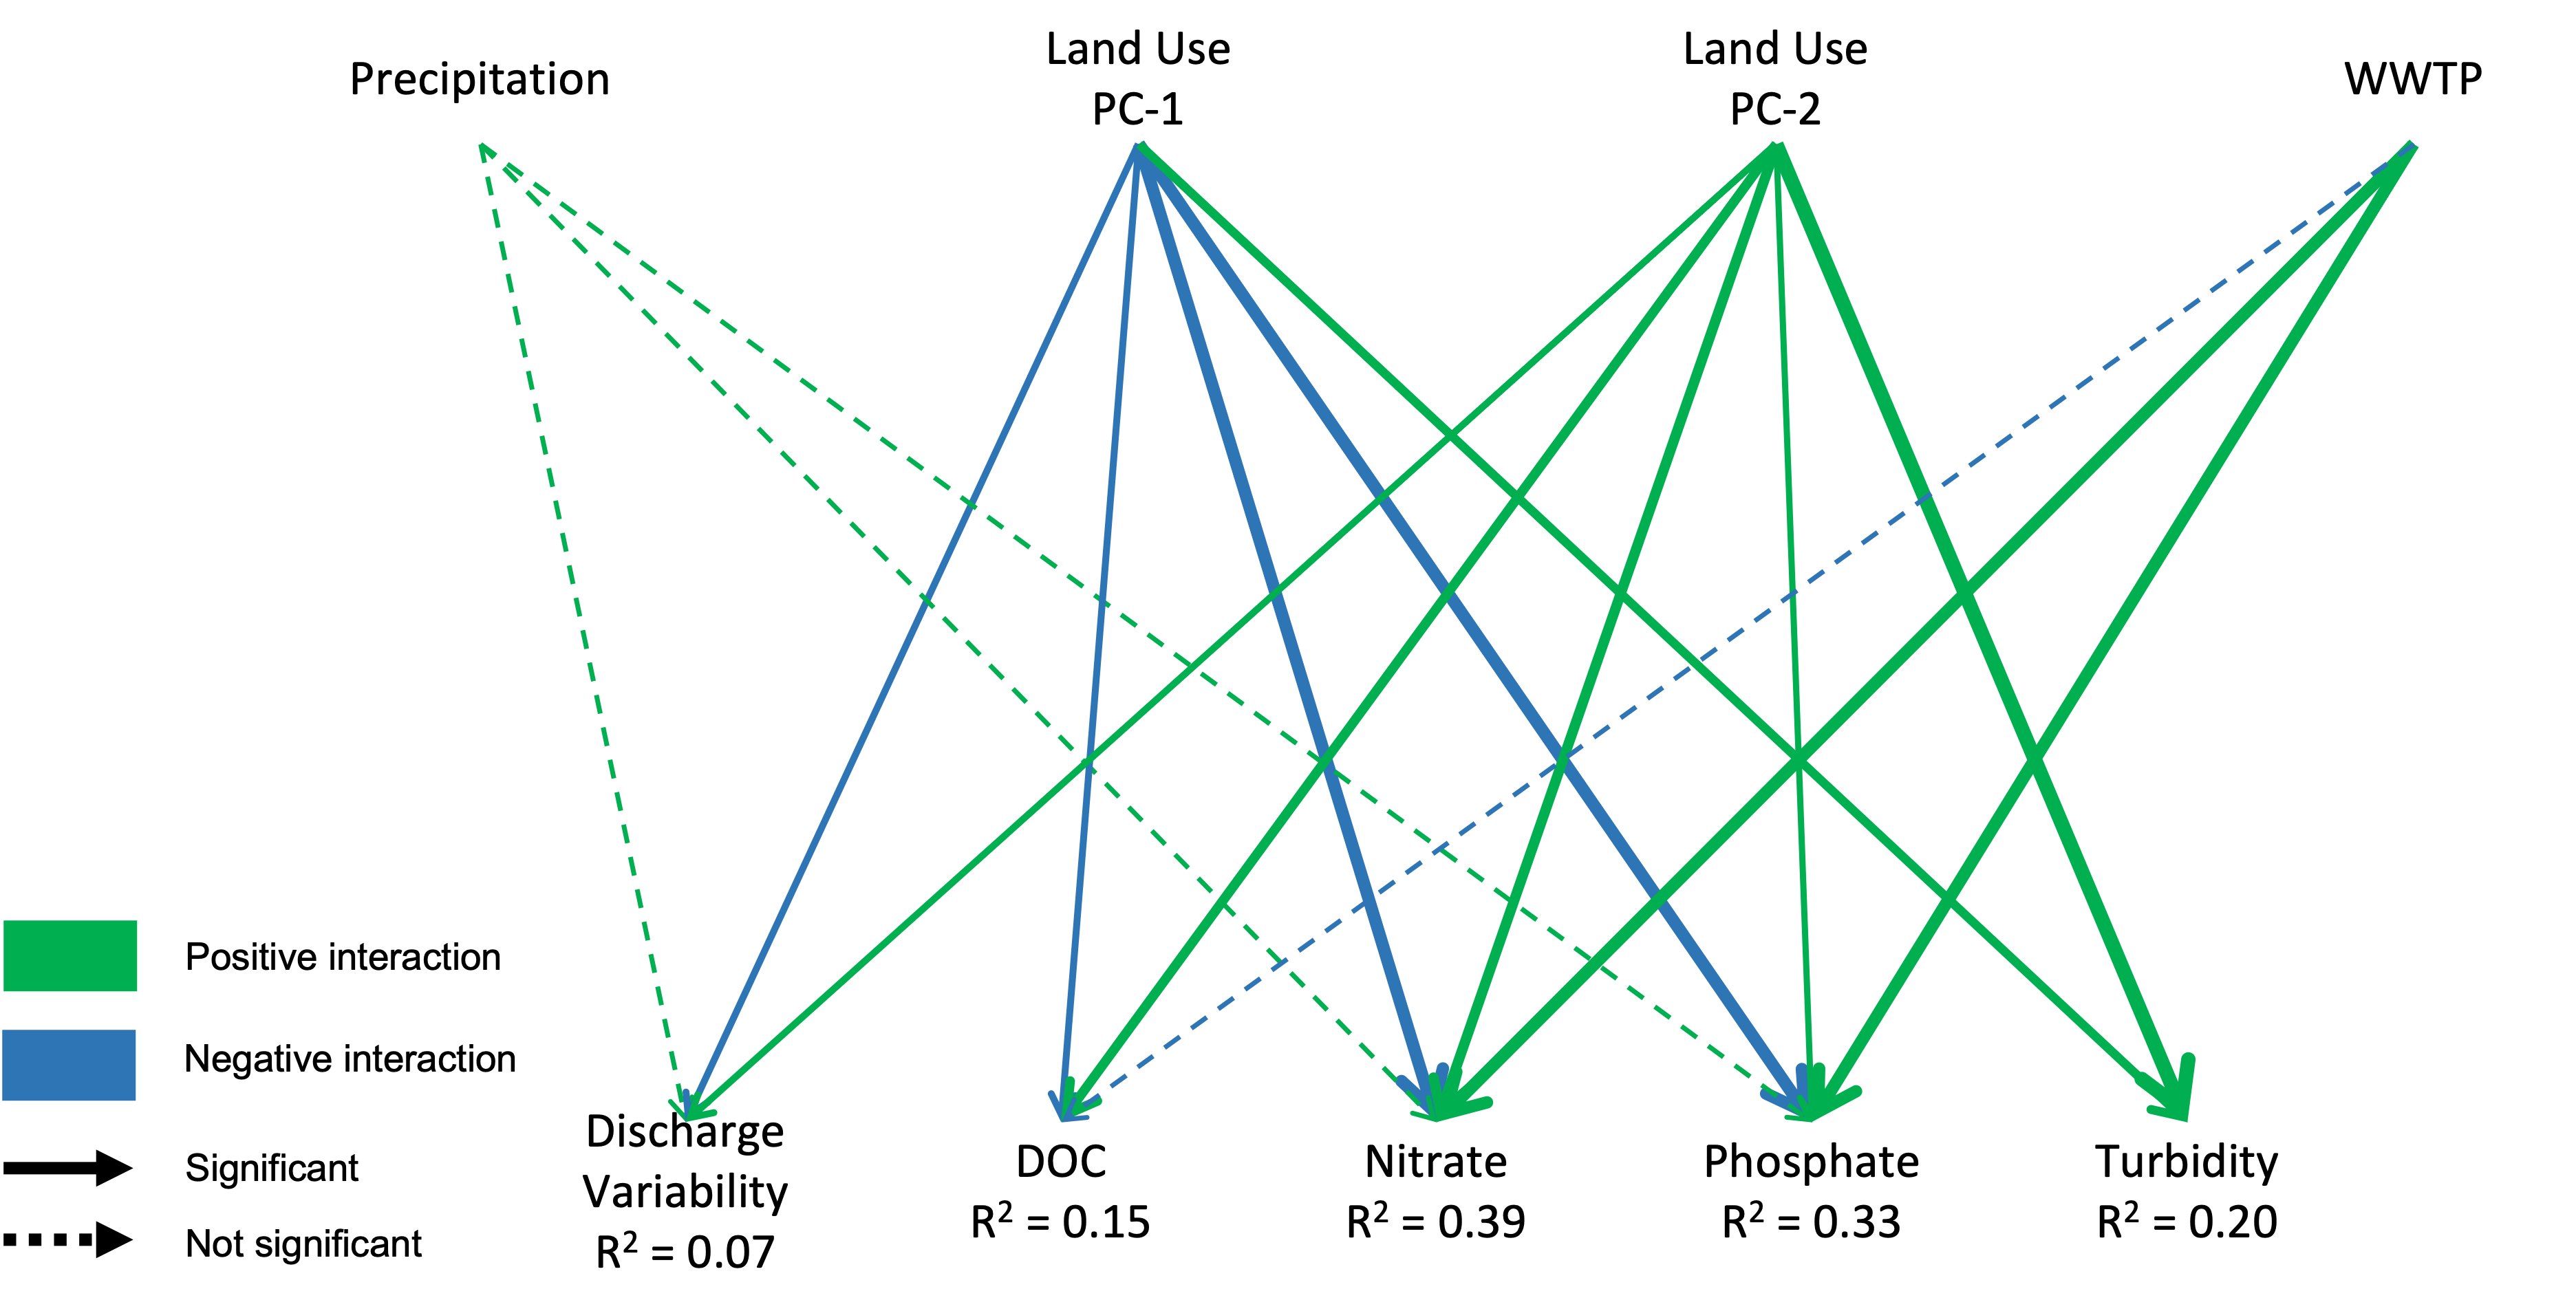
\includegraphics[scale=0.8]{Figs/SEMdrivers.png}
\caption[SEM 2]{\textit{SEM 2}. The land use PCs (PC1 and PC2) and precipitation gradient had a strong impact on proximal drivers (discharge, turbidity, DOC, nitrate, and phosphate).}
\label{Fig:SEMdrivers}
\end{center}
\end{figure}
\end{landscape}

\endinput

%-----------------------------------------------------------------------
% End of chap3.tex
%-----------------------------------------------------------------------


%-----------------------------------------------------------------------
% Beginning of chap4.tex
%-----------------------------------------------------------------------
%
%%%%%%%%%%%%%%%%%%%%%%%%%%%%%%%%%%%%%%%%%%%%%%%%%%%%%%%%%%%%%%%%%%%%%%%%

\chapter[DISCUSSION]{Discussion}
\vspace{-12pt}

% We will want to start with a paragraph re-capping your findings and then go into discussing those main findings.
 Across the coupled land use and precipitation regime gradients, all streams were heterotrophic with rates of ER exceeding GPP. Sites had very low GPP (0.12 to 0.78 \unit{\goxy}) compared to ER across the coupled gradients, with no strong apparent seasonal trends and more daily and year to year variation. There was no apparent trend in nutrient concentrations or GPP. However, ER and DOC generally increased as agricultural land increased and non-agricultural vegetation decreased, moving from semi-arid to mesic.
 
\section{Ecosystem Metabolism}
%see some of the work out of Jen Tanks lab -- she had 2 students work on metabolism in ag streams in Indiana.  We have ag watersheds. They found high rates of GPP (and ER) --- Roley is one and Natalie Griffiths is another

%Found one paper from Griffiths, Roley, Tank, Whiles, Rosi, and Beaulieu for 6 midwestern row-crop drained streams  



%site figures and tables as needed to reference the data you are discussing

% don't site AJU 2018 29 GPP, find different site, 29 may not be real (prob half that, bad K), currently citing stream 6 1st order stream as 25 gO2m-2d-1 GPP
% ask AJU about making Fig 1 from AJU 2018, would be useful in thesis appendix, or in MS

Texas coastal plain streams appear to have relatively low GPP compared to other stream ecosystems (Figure~\ref{fig:GPPBox}). For instance, mean GPP in tropical streams with an open canopy was 2.09 \unit{\goxy} and in a small forested head water stream in Tennessee mean GPP was 1.4 \unit{\goxy} peaking at 10.80 \unit{\goxy} \cite{roberts_multiple_2007, marzolfEcosystemMetabolismTropical2021}. Sub-alpine streams appear to have greater GPP compared to the Texas coastal plain streams as well where GPP from 12 Austrian sub-alpine streams peaked at 25 \unit{\goxy} \cite{ulseth_climate-induced_2018}. Agricultural streams elsewhere also have greater GPP, where in six mid-western row-crop draining streams with high light availability and nutrients, mean GPP was 4.6 \unit{\goxy} peaking at 22.0 \unit{\goxy} \cite{griffithsAgriculturalLandUse2013}. In comparison, 33 Austrian streams with a mix of forested, agriculture, and urban land uses were slightly similar to slightly higher than Texas coastal plain streams where GPP ranged from 0.01 to 3.3 \unit{\goxy} \cite{fus_land_2017}. Rates of GPP from these Texas coastal streams were most similar to those of closed canopy tropical streams (0.57 \unit{\goxy}),  \cite{marzolfEcosystemMetabolismTropical2021}. Canopy cover could explain some of the limitation of light, for sites where canopy cover was low, turbidity likely decreased light reaching the benthos, where most of the primary production would take place (average turbidity ranged from 15-141 NTU). This suggest these streams were likely light limited, resulting in low rates of GPP \cite{hall_turbidity_2015,honiousTurbidityStructuresControls2021, marzolfEcosystemMetabolismTropical2021}. Another contributing factor to low GPP in these ecosystems may be caused by sandy substrate and frequent bed movement. Across the coupled gradients, a majority of sites had sandy substrate. In a desert stream in Arizona, low GPP (0.15 to 0.29 \unit{\goxy}) was attributed to bed movement caused by sandy substrate disrupting primary producers \cite{uehlingerHeterotrophicDesertStream2002}. Again in a rural Australian stream, low GPP (0 to 0.5 \unit{\goxy}) was also attributed to bed movement caused by sandy substrate \cite{atkinsonSedimentInstabilityAffects2008}. In streams with high bed movement, GPP is often suppressed due to disturbance to primary producers \cite{uehlingerEcosystemMetabolismDisturbance1998, uehlingerHeterotrophicDesertStream2002, atkinsonSedimentInstabilityAffects2008}. 

Within sites, daily variation of GPP exceeded that of seasonal variation (Figure~\ref{Fig:MetabStacked}). There was not strong seasonal variation or a peak of GPP in the spring or summer within sites. The lack of seasonal trends in GPP appears to be uncommon in other stream ecosystems. For instance, in a small forested Tennessee stream GPP peaked during spring before leaf out (0.01 to 10.80 \unit{\goxy}), which was attributed to an increase in light due to longer days in spring prior to canopy leaf out \cite{roberts_multiple_2007}. In 12 Austrian sub-alpine streams GPP peaked in spring after snow melt (0.01 to 25 \unit{\goxy}) which was also attributed to increased light \cite{ulseth_climate-induced_2018}. In 6 mid-western row-crop drained streams, GPP also peaked in the spring (0.1 to 22.0 \unit{\goxy}) which was also attributed to high light availability \cite{griffithsAgriculturalLandUse2013}. Again, in an analysis of 222 stream and rivers across the Unites States, seasonal changes in light and flow regimes were found to be the strongest drivers of GPP \cite{bernhardtLightFlowRegimes2022}.  In the subtropical Texas coastal plains region, where there is a more subtle shift in seasons, compared to temperate ecosystems, along with high turbidity in these streams, may be attributed to low GPP and lack of strong seasonal peaks in GPP seen in other stream ecosystems.

%Comment from AJU, think about substrate, these are sandy streams compared to more rock of pebble substrate (lots of bed movement, disrupting producers?). Think about Urs uhlinger scoured paper, hard substrate, maybe nancy grimm 1980s(?) paper, but used chambers

%Our ER was close to ER from the Marzolf tropical ag impacted stream, not overall review. Also found a negative relationship between SPR and ER, ag stream had 0.25\unit{\mg\per\l} SPR (highest in marzolf study) (similar to our P)

%we need a topic sentence here regarding ER -- something perhaps along the lines that ER rates from the TX coastal plain streams were slightly lower, but within range (?) of estimates of ER from other stream ecosystems.  Then go into comparing rates from other studies has you have done ---
ER rates from these Texas coastal plain streams were lower, but within range (-0.4 to -29.0 \unit{\goxy}) of estimates of ER from other stream ecosystems \cite{bernot_inter-regional_2010}. The median ER rates across these Texas coastal plain streams were similar to estimates of ER from an agriculturally impacted tropical stream in Costa Rica (-0.5 to -0.8 \unit{\goxy}) \cite{ortega-pieckAgriculturalInfluencesMagnitude2017}.
However, median ER of all sites was lower than estimates of ER from tropical streams with a mix of open and closed canopy (-4.30 \unit{\goxy}), six mid-western row-crop drained streams (-0.9 to -34.8 \unit{\goxy}), eight streams with a mix of agriculture, urban, and reference land uses across the Unites States (-2 to -8 \unit{\goxy}), a small forested head water stream in Tennessee (-0.99 to -16.01 \unit{\goxy}), and in 12 streams across an Austrian sub-alpine catchment (-0.04 to -54.2 \unit{\goxy}) \cite{marzolfEcosystemMetabolismTropical2021, bernot_inter-regional_2010, mulholland_inter-biome_2001, ulseth_climate-induced_2018, roberts_multiple_2007, griffithsAgriculturalLandUse2013}. As nutrients and DOC concentrations were relatively high to fuel microbial metabolism (Table \ref{tab: Nutrients}), I would have expected greater rates of ER; however, rates of ER were on the lower end of the range reported from other ecosystems \cite{bernot_inter-regional_2010, mulholland_inter-biome_2001, ulseth_climate-induced_2018, roberts_multiple_2007, griffithsAgriculturalLandUse2013}. These lower than expected rates of ER may be explained by the lack of hyporehic exchange caused by low channel slope. Streams with low slope have decreased hyporehic exchange where an estimated 50-85\% of of ER fluxes originate  \cite{stanfordEcosystemPerspectiveAlluvial1993, naegeliContributionHyporheicZone1997,fellowsWholeStreamMetabolism2001, mulhollandEvidenceThatHyporheic1997}.
 

% one reason why the SEM model does not work is because we have very little variation in GPP in ER at the monthly level and across sites -- so if nothing varies, the changes in our regional and proximal drivers wouldn't correlate with GPP and ER.

\section{DOC and Nutrients}

Across most sites, DOC concentrations increased along the precipitation gradient. This trend was expected, as increasing DOC concentrations are linked to increases of terrestrial primary production \cite{meybeckCarbonNitrogenPhosphorus1982, mulhollandGroupReportWhat1989, jonesLongtermPerspectiveDissolved1996}. However, the driest site, TRC and the second most mesic site, EMC did not follow this pattern. TRC is dominated by a dense, intact riparian zone comprised of native shrub vegetation, anoxic stream water (DO < 0.5 \unit{\mg\per\l}) 75\% of the time, and an average discharge of 0.03 m$^3$/s. With possible low hyporheic exchange, lack of mineralization of DOC may have caused the DOC concentrations to be higher than found at other sites. The second site that did not follow the pattern was EMC, this site has a watershed that is dominated by agriculture and has a sandy riparian zone, this may have led to a decrease in DOC compared to other sites. The sandy sediment in the riparian zone contains less organic carbon than riparian zones composed of soil \cite{boix-fayosSedimentFlowPaths2015}. The increase in DOC across the precipitation gradient did not drive an increase in ER. A temporal miss-match in the monthly sampling schedule potentially caused the inability to link interactions between DOC and ER.


%here we also would need a topic sentence to better encapsulate your discussion.  Rather than have SFC as your topic sentence -- 'Nutrient concentrations did not appear to drive variation in GPP and ER'.  As you are using this paragraph to 1. introduce discussion regarding nutrient concentrations and 2. the effect of said nutrients on rates of GPP and ER
Nutrient concentrations did not drive variation in GPP and ER. All sites, except SFC, had similar concentrations of ammonium amd nitrate, with  no apparent trend across the gradients (Table \ref{tab: Nutrients}). Sites receiving WWTP effluent had increased level of nitrate. SFC is predominantly waste water dependent, likely contributing to increased nitrate and phosphate concentrations. This increase in nutrients may have lead to SFC having the second highest ER for these coastal streams (-2.60 \unit{\goxy}). Generally, increases in nutrient concentrations fuel microbial respiration and lead to increased ER \cite{ramirezEffectsStreamPhosphorus2003}. However, the results from the SEM (Figure~\ref{Fig:SEMmetab}) indicate there was not a significant impact of nutrient concentrations on GPP or ER. Previous studies on eight and nine streams with a mix of agriculture, urban, and reference land uses across the Unites States and Puerto Rico and 83 streams across the global tropics have also been unable to relate rates of ecosystem metabolism to nutrient concentrations \cite{mulholland_inter-biome_2001,bernot_inter-regional_2010, marzolfEcosystemMetabolismTropical2021}. The findings from this study and others suggest weekly or monthly nutrient measurements may be insufficient for linking nutrient concentrations to changes in ecosystem metabolism and more frequent measurements of nutrient concentrations are needed to link the effects of nutrients to daily estimates of GPP and ER \cite{bernot_inter-regional_2010, fus_land_2017}.


\section{Discharge}

Across the precipitation and land use gradients, WMC had the highest discharge, while SFC had the most flow variability (Table~\ref{tab:Q}). All sites exhibited quick increases in discharge from frequent precipitation events, with equally quick decreases after precipitation events. Frequent precipitation events, which increase stream discharge, leads to scouring of primary producers and increases in turbidity, which may reduce GPP \cite{uehlinger_resistance_2000, hall_turbidity_2015}. However, the low GPP in the Texas coastal streams may already be light limited without increased turbidity from high flows. 


\section{Precipitation and Land use Gradients}

With monthly measurements of nutrients, DOC, and turbidity, there was a strong influence of land use proximal drivers of ecosystem metabolism, with land use driving changes in nitrate, phosphate, ammonium, and turbidity. However, there was not an influence of DOC, nitrate, phosphorous, ammonium, and turbidity on GPP and ER.  The inability to find a link between proximal drivers and ecosystem metabolism suggest the snap-shot sampling of nutrients, DOC, and turbidity was too limited to detect responses of ecosystem metabolism to changes in proximal drivers \cite{bernot_inter-regional_2010}. The low variation in GPP and ER (Table \ref{metab}) may have also prevented linking drivers to ecosystem metabolism. Additionally, these streams had intact riparian zones and were likely light limited, which may have limited the response of ecosystem metabolism to changes in land use \cite{jankowskiLandUseChange2021, bernhardtLightFlowRegimes2022, griffithsAgriculturalLandUse2013}.

\section{Conclusion}

%Did a quick lit search, tons of ppl refer to this area as subtropical with no citations

%I broke this into 2 paragraphs, because the flow felt off reading it all together. I may need help word smithing. But let me know what you think
While I was able to parse out the effect of regional drivers (land use and precipitation regimes) on proximal drivers of ecosystem metabolism (ie. nutrients, DOC, and turbidity), I was unable to elucidate the combined effects of precipitation and land use gradients on stream ecosystem metabolism. This suggest the two coupled gradients, land use and precipitation regime, may mask the combined effects on stream ecosystem metabolism. Future work should focus on the use of high frequency measurements of proximal drivers to attempt to parse out drivers of ecosystem metabolism in subtropical streams. 




A majority of research on stream ecosystem metabolism comes from temperate regions, with tropical and subtropical regions being understudied \cite{marzolfEcosystemMetabolismTropical2021}. These subtropical Texas coastal plains streams provide valuable insight into how subtropical streams may differ from their more studied temperate counterparts. These low estimates of GPP suggest that Texas coastal streams likely rely heavily on allochthonous rather than autochthonous carbon sources as a basal resource. These are slow, flat streams, which have low GPP and low to moderate ER. These streams do appear to function differently than their more temperate counterpart. But in light of global change, teasing apart what drives ecosystem metabolism will be of importance given that GPP and ER modulate carbon, nutrient fluxes, and even basal food resources.




% Also, we want to weave in the strengths and weaknesses of this study.  Often it is fair to discuss the potential weaknesses of the study towards the end -- Also think about future directions as well. I like where your conclusion is going, that is the idea there -- now you may also want to think about what we would need to know in terms of discerning land use, for instance

%Also, as I am typing this -- I wonder if land use is similar to biomes. Referencing Bernhardt et al. Metabolic Regime paper and some of Walter Dodd's work - 'do streams have biomes', perhaps another reason we did not see a strong connection with ppt gradient and land use is because the phenology of the terrestrial ecosystem is not typed with essentially the phenology of the stream ecosystem. And as you allude in your conclusion text -- local drivers (light, riparian vegetation) may be of more importance than large-scale drivers.  I would have to read through Dodds paper again - but I think they concluded that streams did not have biomes. As for the metabolic regime of coastal TX streams -- dampened seasonal trends?  Just a few thoughts...



% With continued climate change, it is uncertain how stream ecosystem functions such as carbon storage and transport will respond.





\endinput

%-----------------------------------------------------------------------
% End of chap4.tex
%-----------------------------------------------------------------------

%%%%%%%%%%%%%%
%%%%% END  %%%%%%
%%%%%%%%%%%%%%

\clearpage

%%%%%%%%%%%%%%%%%%%%%%%
% REFERENCES
%  Bibliography prepared with BibTeX using amsplain or amsalpha.
% I modified amsplain and amsalpha to abbreviate the first name of each author.
\addcontentsline{toc}{chapter}{REFERENCES}

\bibliographystyle{amsplain} 
%\bibliographystyle{babamspl} 

% \bibliographystyle{abbrvamsplain}
 \bibliography{Bibliography}
%%%%%%%%%%%%%%%%%%%%%%%

\backmatter
%%%%%%%%%%%%%%%
% APPENDIX
%%%%%%%%%%%%%%%
%
%%%%%%%%%%%%%%%%%%%%%%%%%%%%%%%%
% The following two lines are old and must not be uncommented.
%%%%%%%%%%%%%%%%%%%%%%%%%%%%%%%%
%\addtocontents{toc}{%
 %\protect\noindent\normalfont APPENDIX\protect\par}
%%%%%%%%%%%%%%%%%%%%%%%%%%%%%%%%
%
%%%%%%%%%%%%%%%%%%%%%%%%%%%%%%%%
% Since the format of the CHAPTER headings was changed,
% I need to manually change the format for the Appendix heading.
\titleformat{\chapter}[display]
{\normalfont\bfseries\filcenter}
{APPENDIX \thechapter}
{0ex}
{\titlerule[0pt]
\vspace{0ex}%
}
[\vspace{0ex}%
{\titlerule[0pt]}]
\titlespacing{\chapter} {0pt}{-20pt}{12pt}
%%%%%%%%%%%%%%%%%%%%%%%%%%
%
%%%%%%%%%%%%%%
%% MODIFY ME %%%%%
%%%% BEGIN %%%%%%
%%%%%%%%%%%%%%
% Comment the following lines if there are no appendices
%
\begin{appendices}

%-----------------------------------------------------------------------------
% Beginning of appendix1.tex
%-----------------------------------------------------------------------------
%
%%%%%%%%%%%%%%%%%%%%%%%%%%%%%%%%%%%%%%%%%%%%%%%%%%%%%%%%%%%%%%%%%%%%%%%%

\chapter{APPENDIX A}

\section{Metabolism Data}

Below are graphs of temporal variation for all sites for GPP (green lines), ER (orange lines), and NEP (black lines) across the coupled gradients. Sites are arranged arid to mesic top down. 


\begin{figure}[htb]
\begin{center}
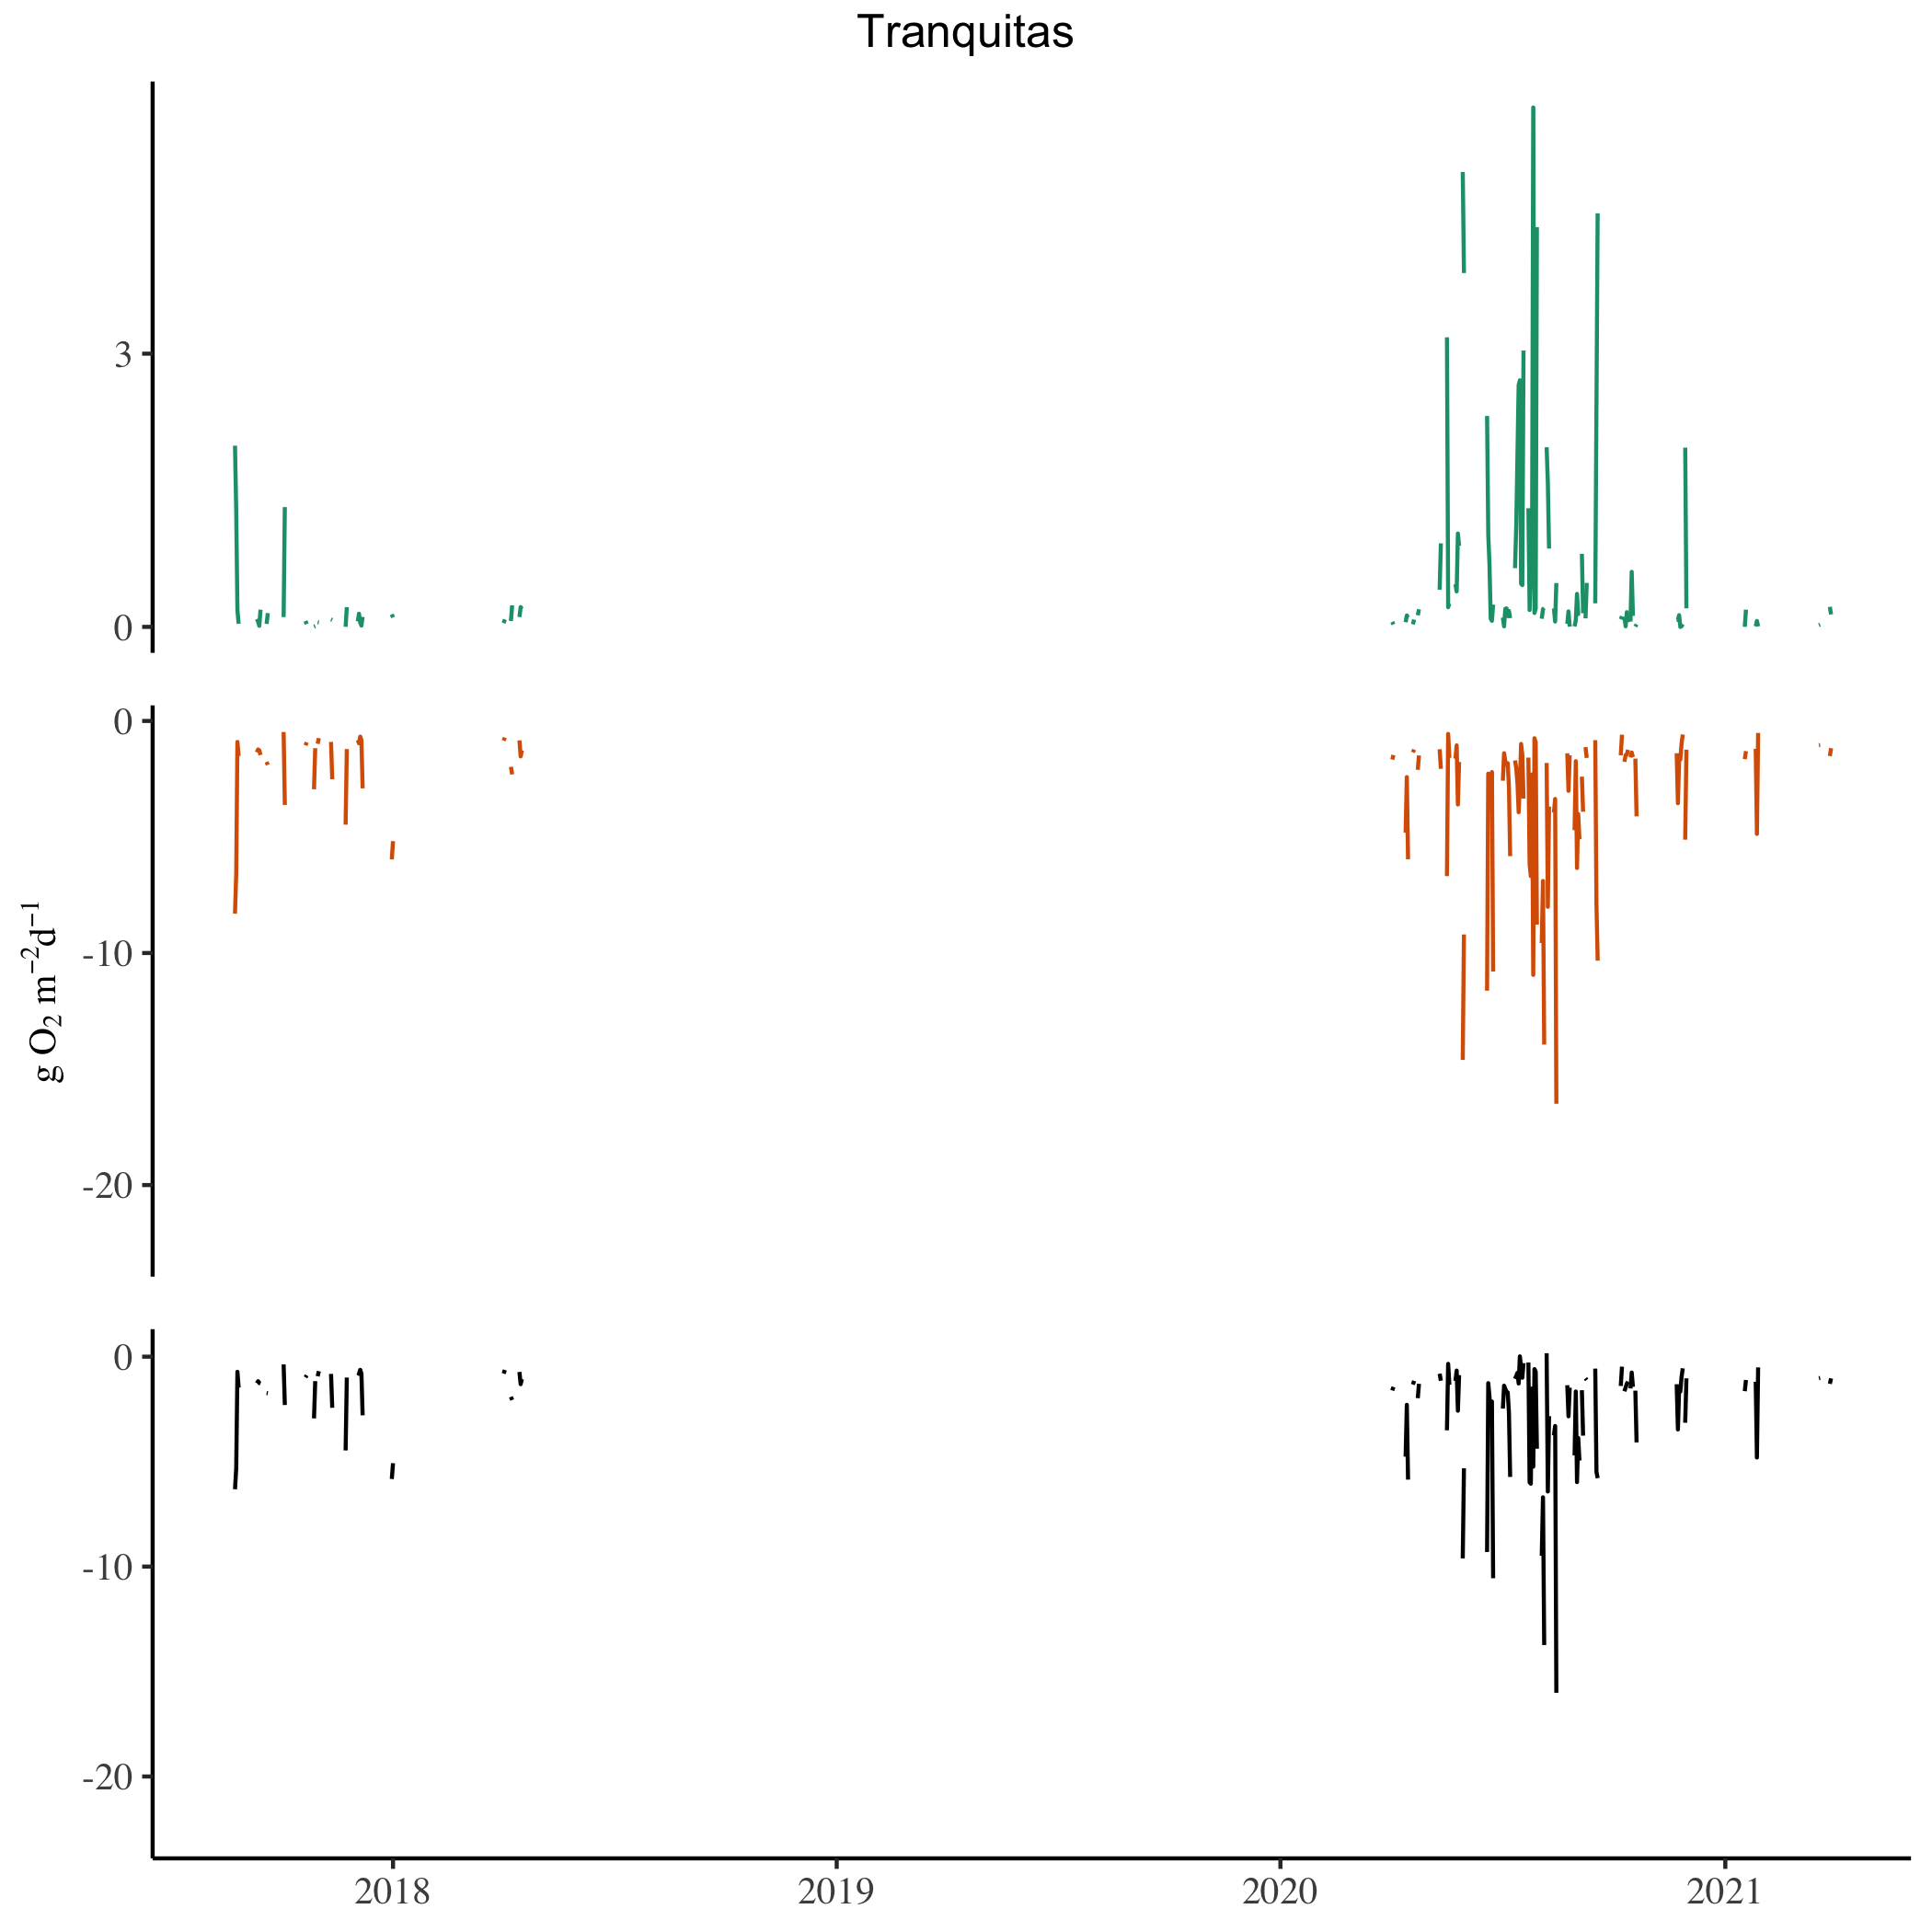
\includegraphics[scale=0.2]{Figs/TRC.png}
\caption{Tranquitas Creek.}
\label{Fig:TRC}
\end{center}
\end{figure}

\begin{figure}[htb]
\begin{center}
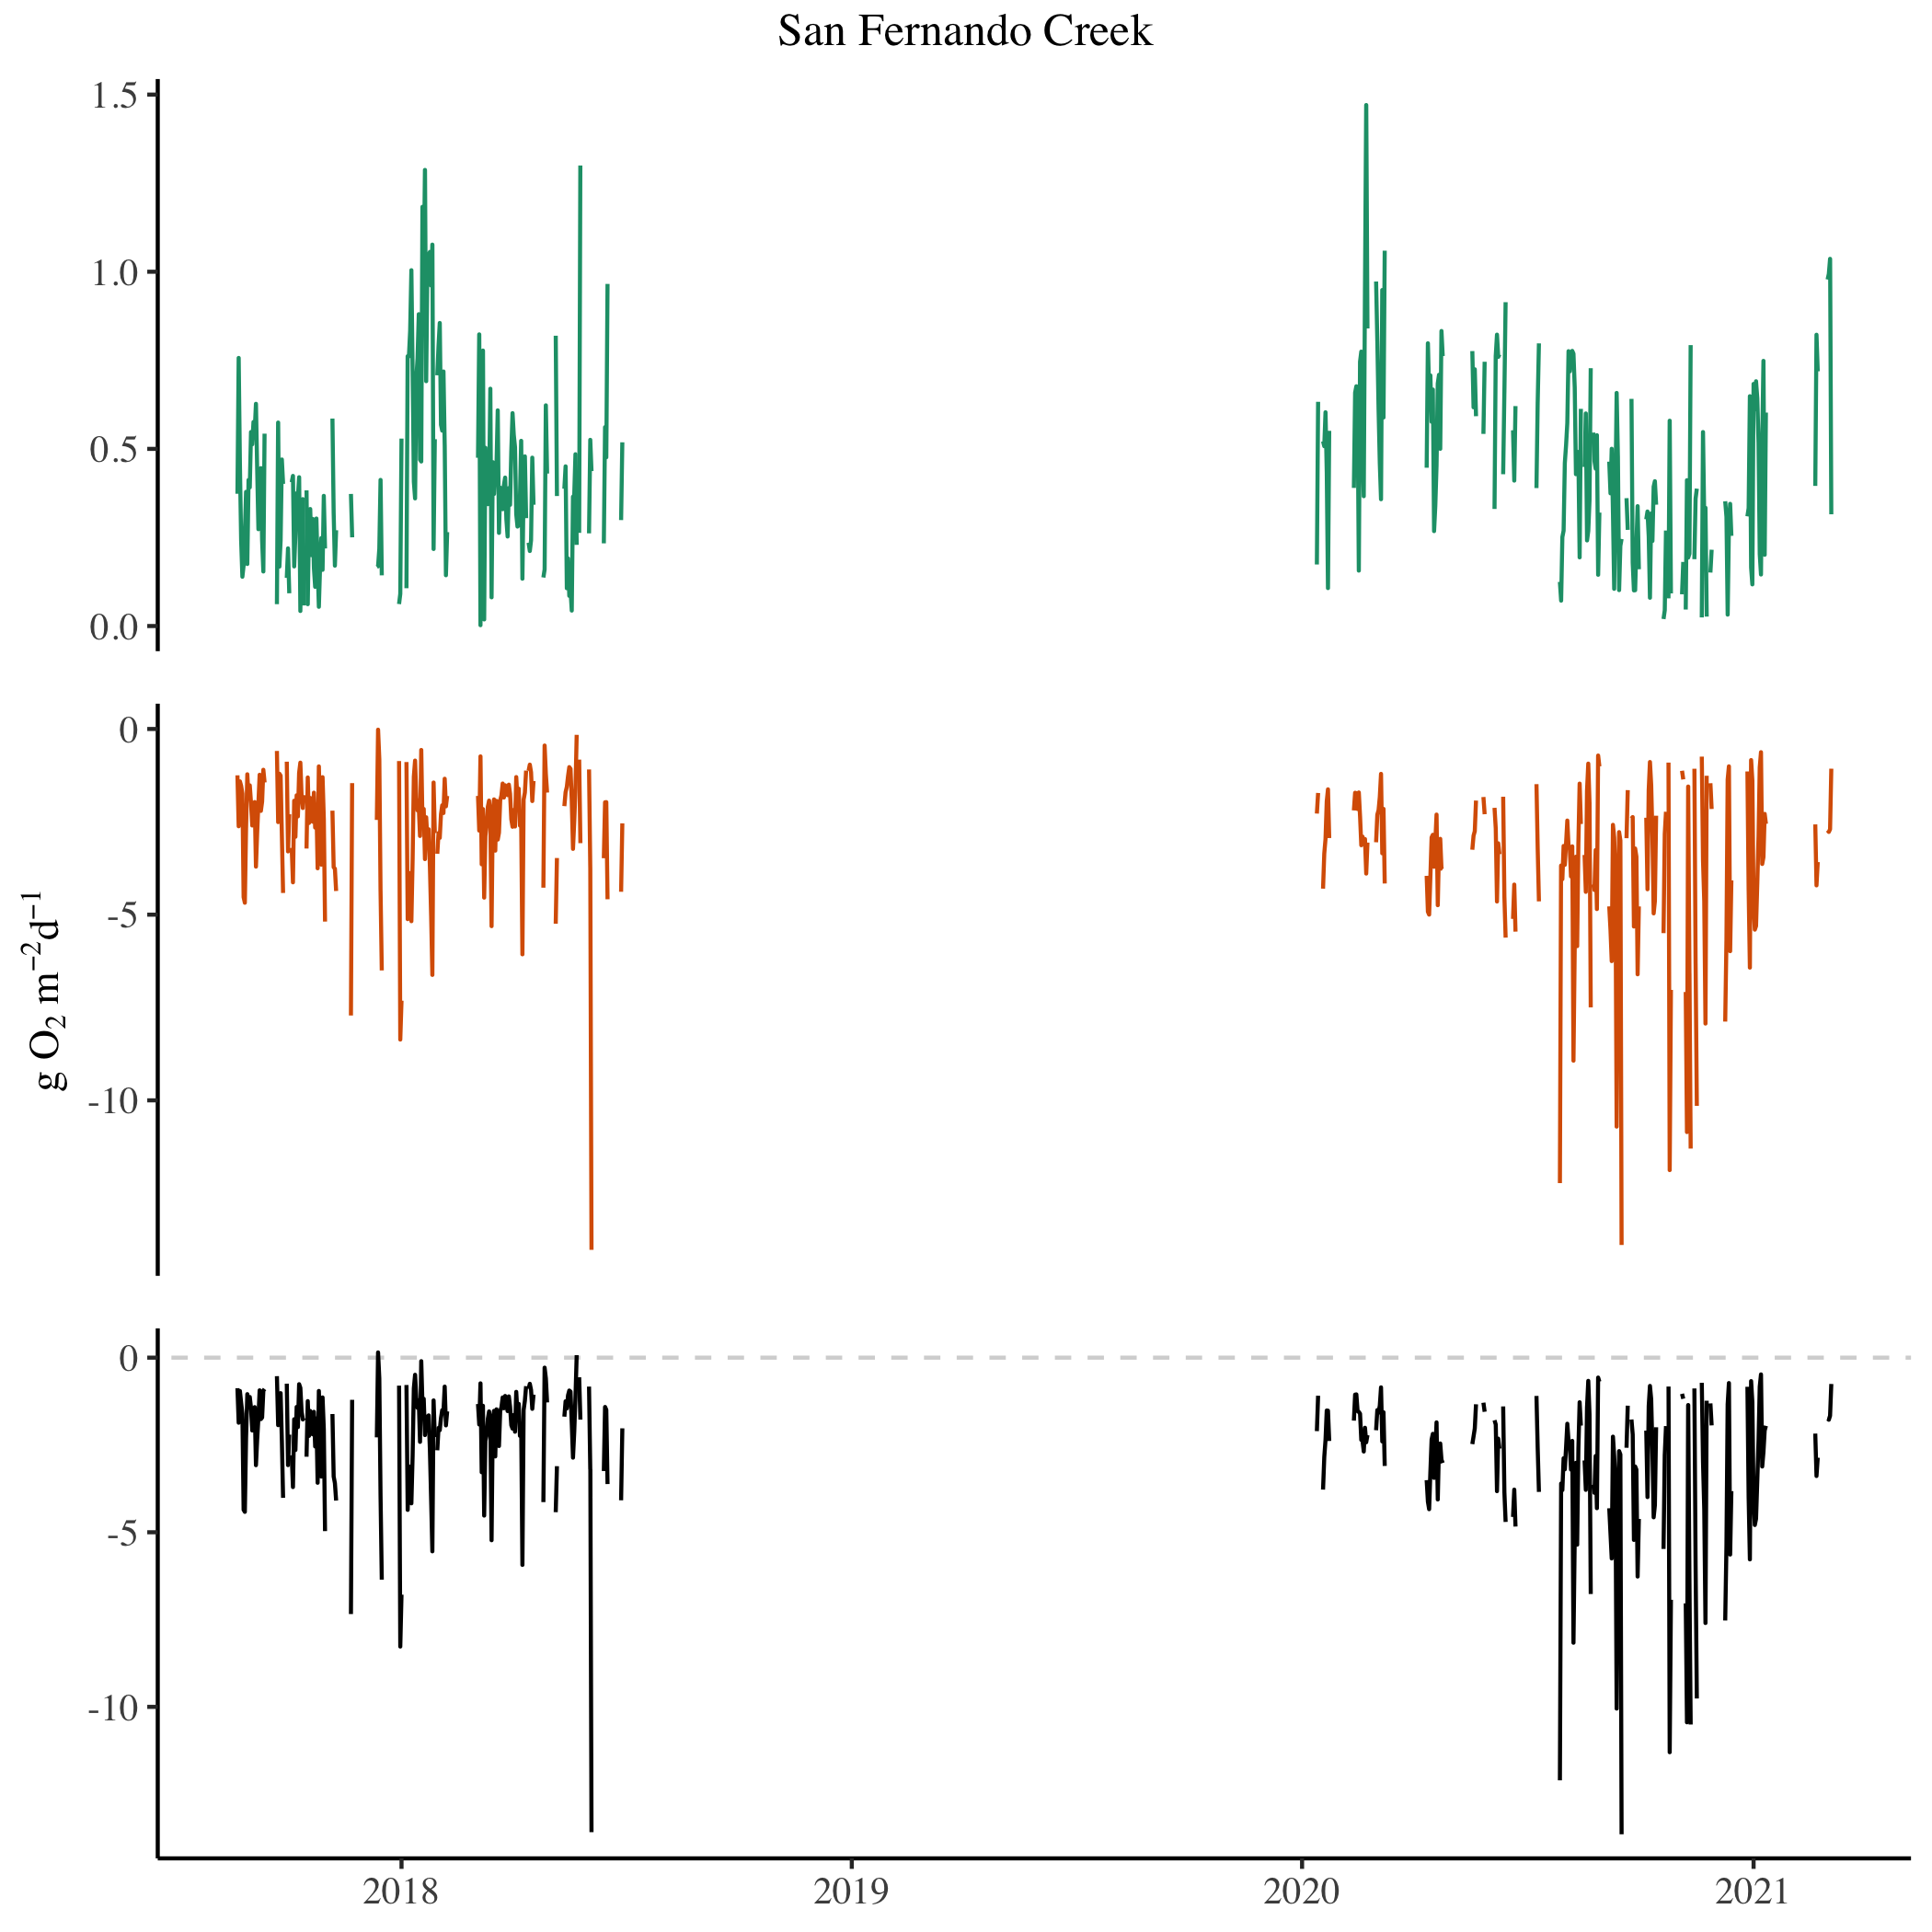
\includegraphics[scale=0.2]{Figs/SFC.png}
\caption{San Fernando Creek}
\label{Fig:SFC}
\end{center}
\end{figure}

\begin{figure}[htb]
\begin{center}
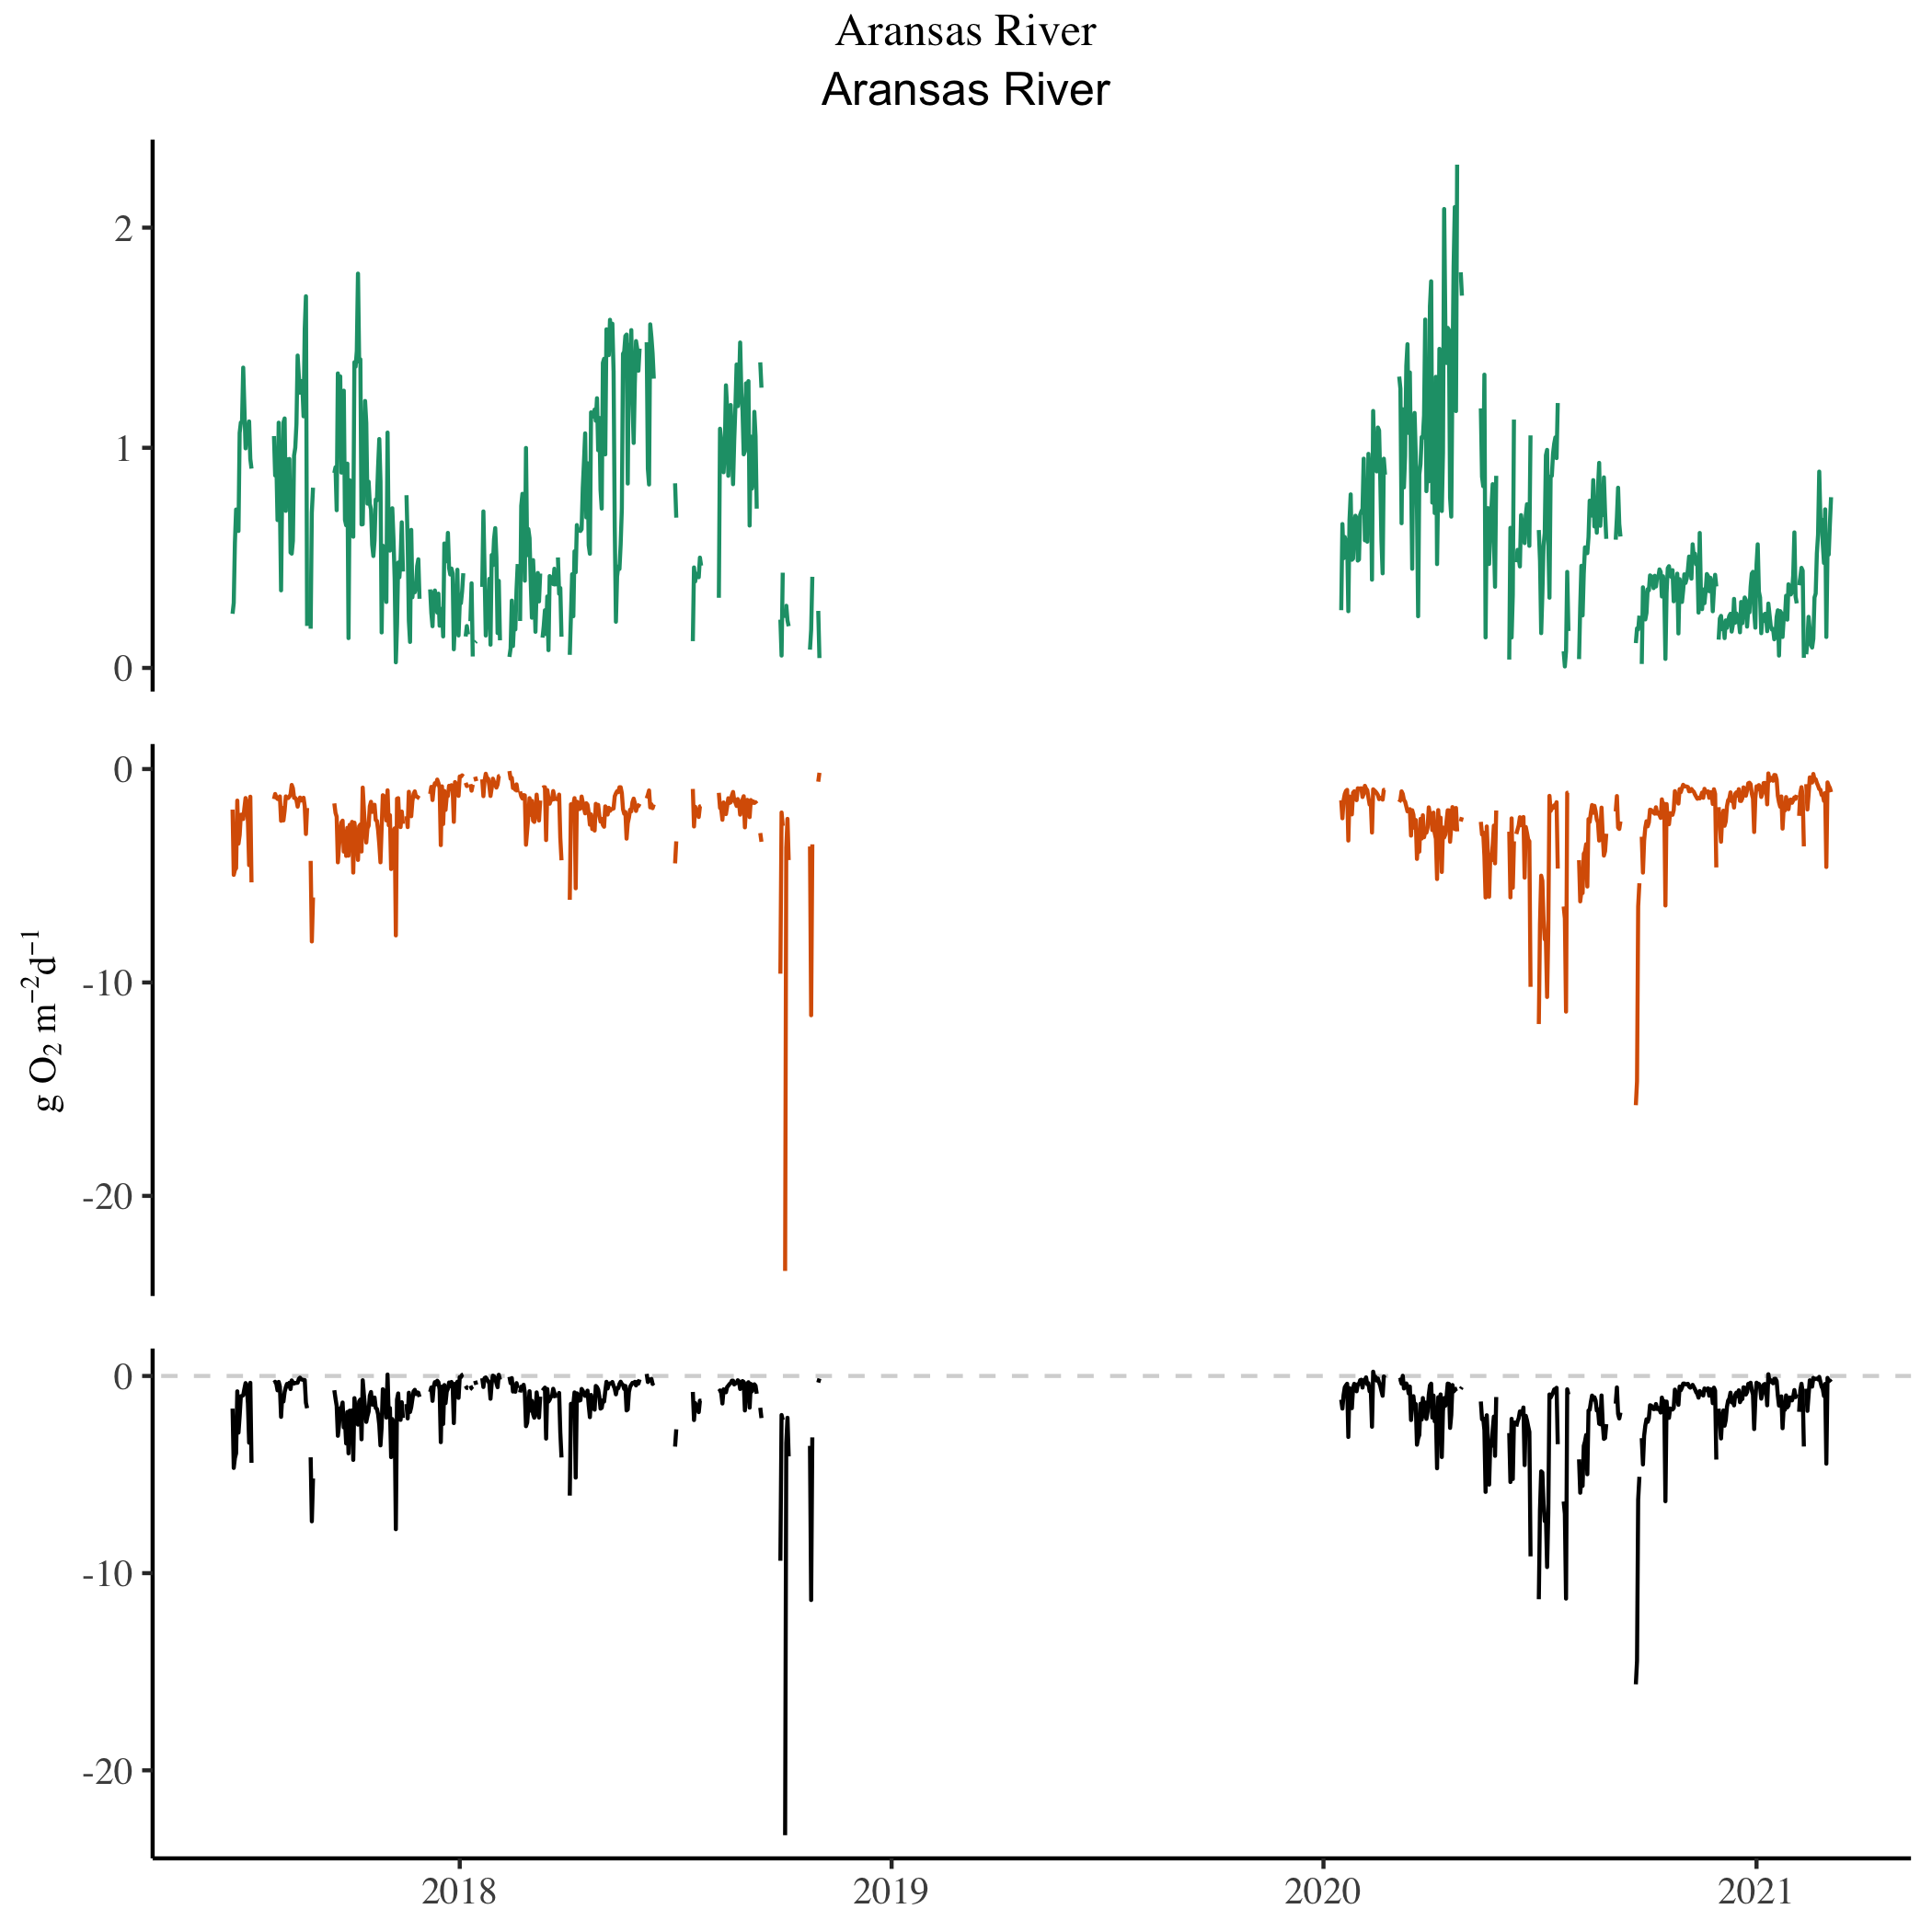
\includegraphics[scale=0.2]{Figs/AR.png}
\caption{Aransas River}
\label{Fig:AR}
\end{center}
\end{figure}

\begin{figure}[htb]
\begin{center}
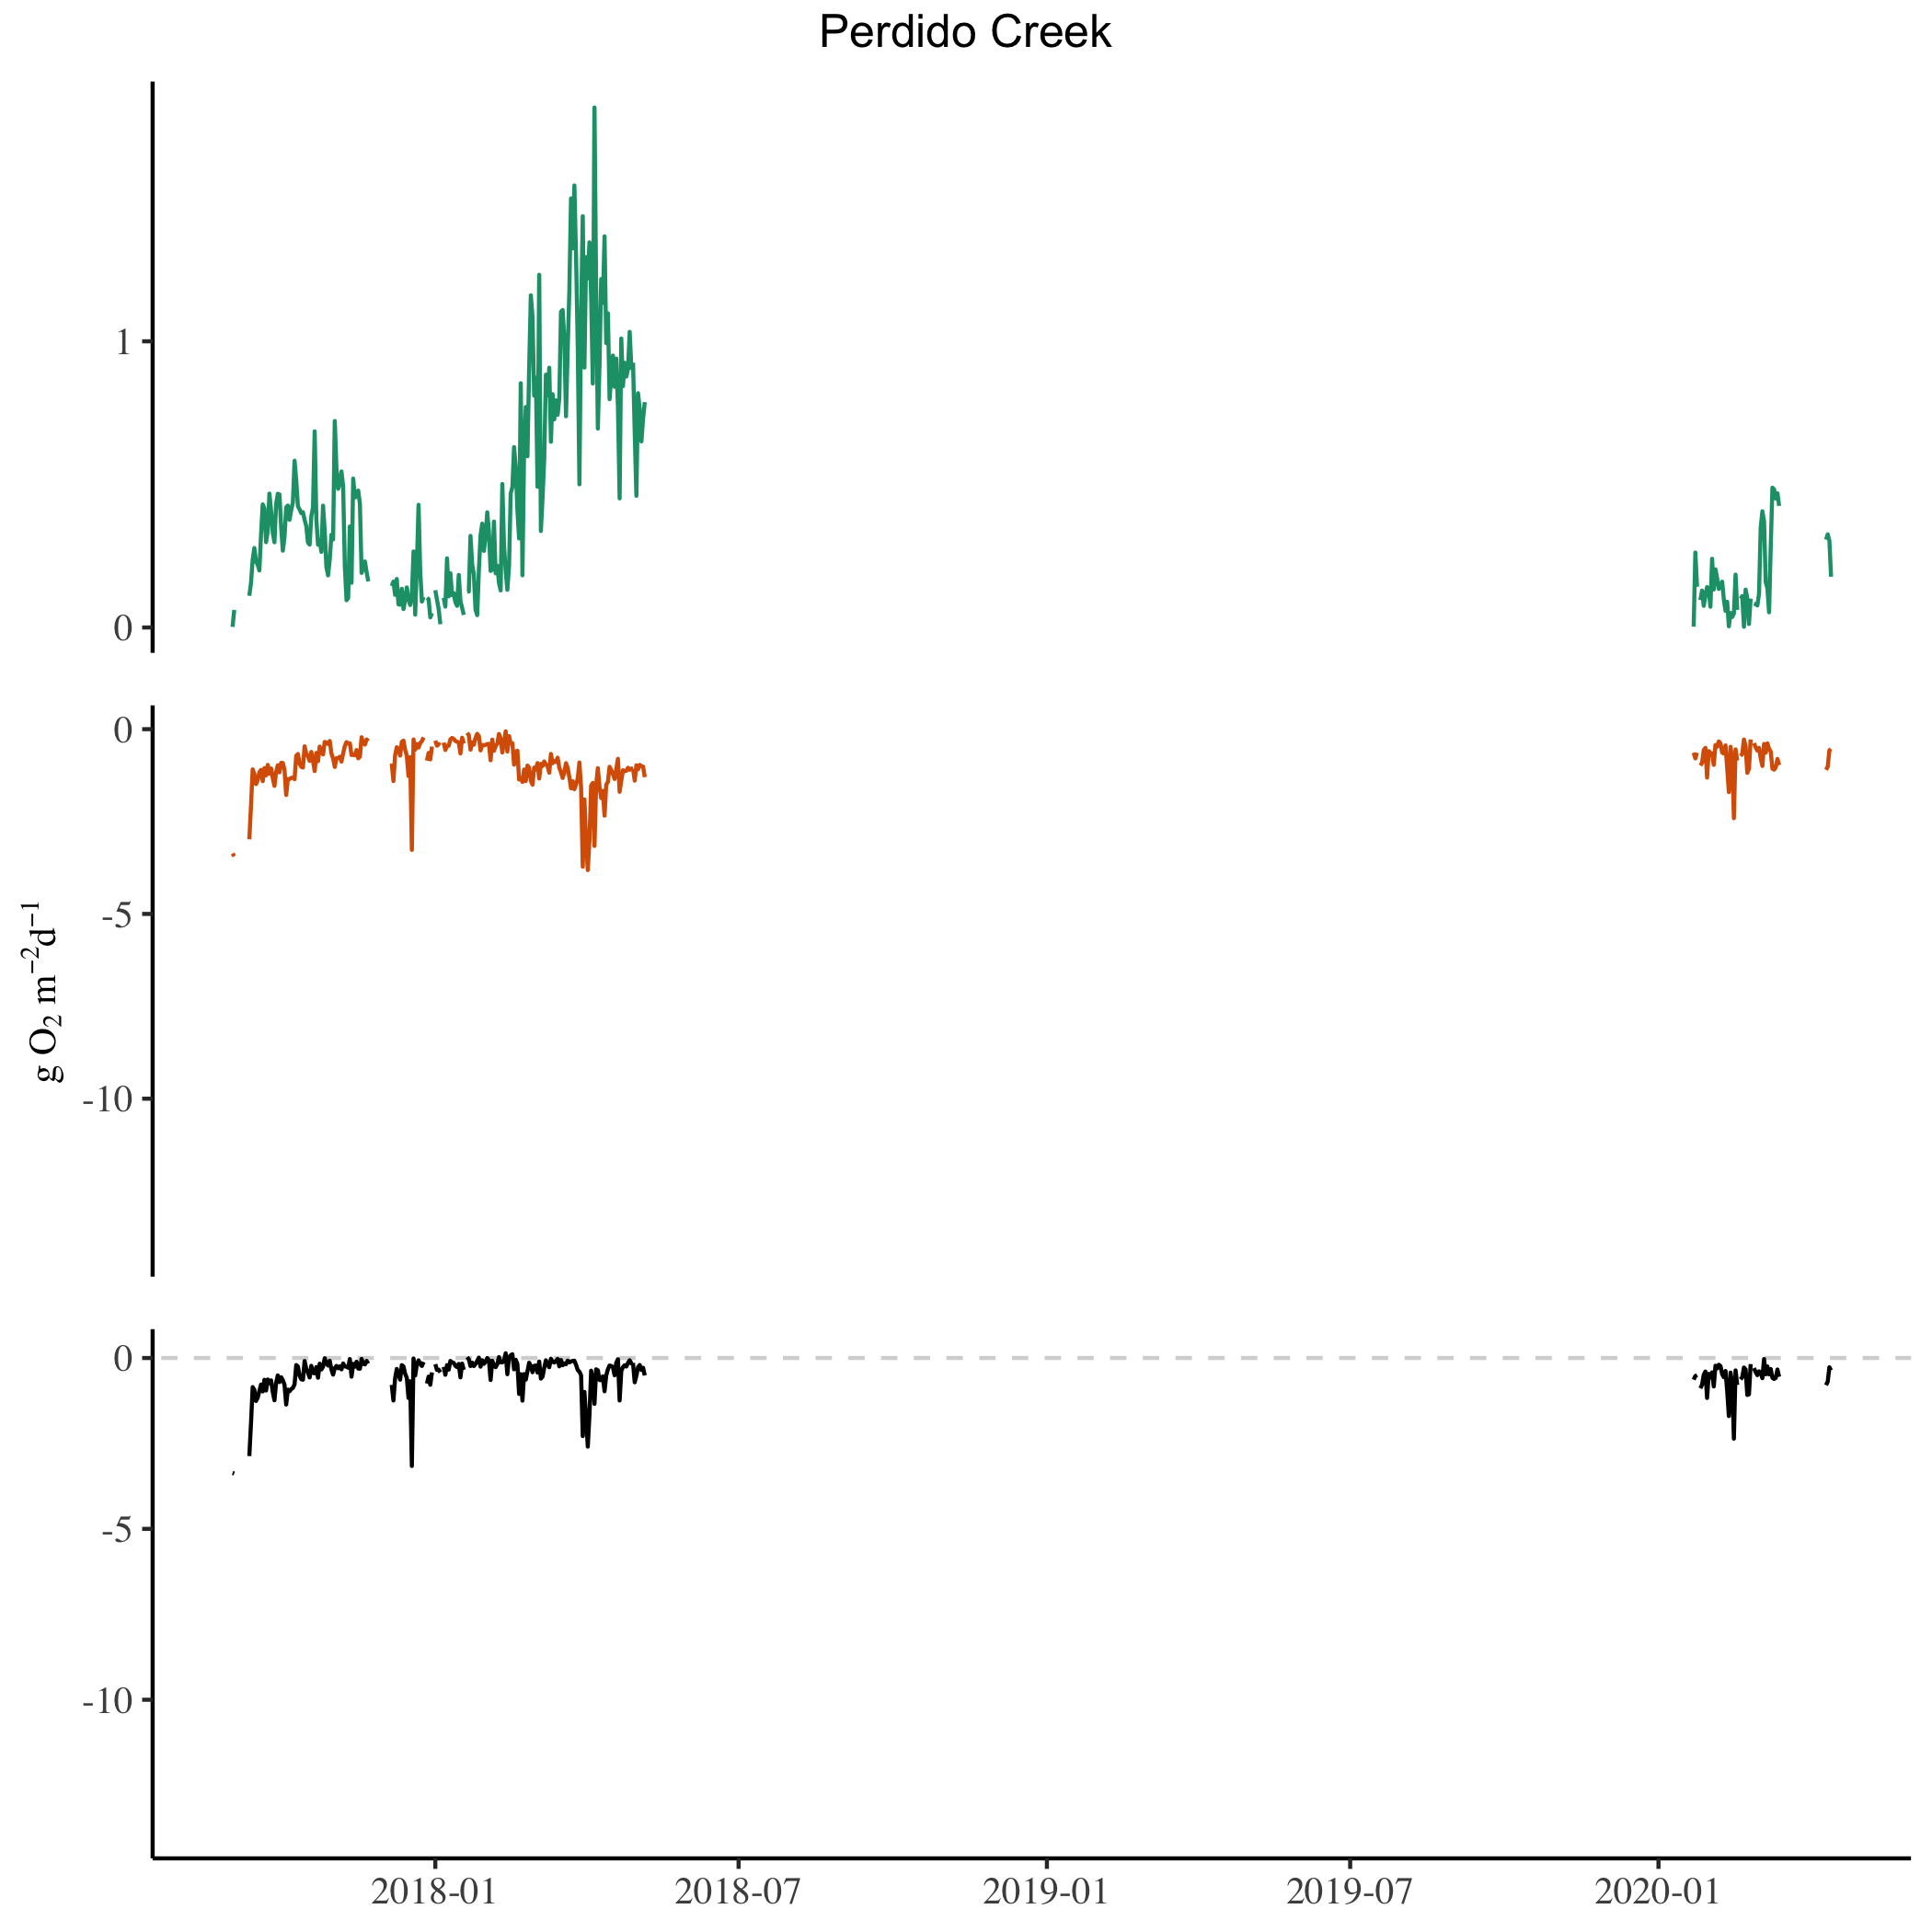
\includegraphics[scale=0.2]{Figs/PDC.png}
\caption{Perdido Creek}
\label{Fig:PDC}
\end{center}
\end{figure}

\begin{figure}[htb]
\begin{center}
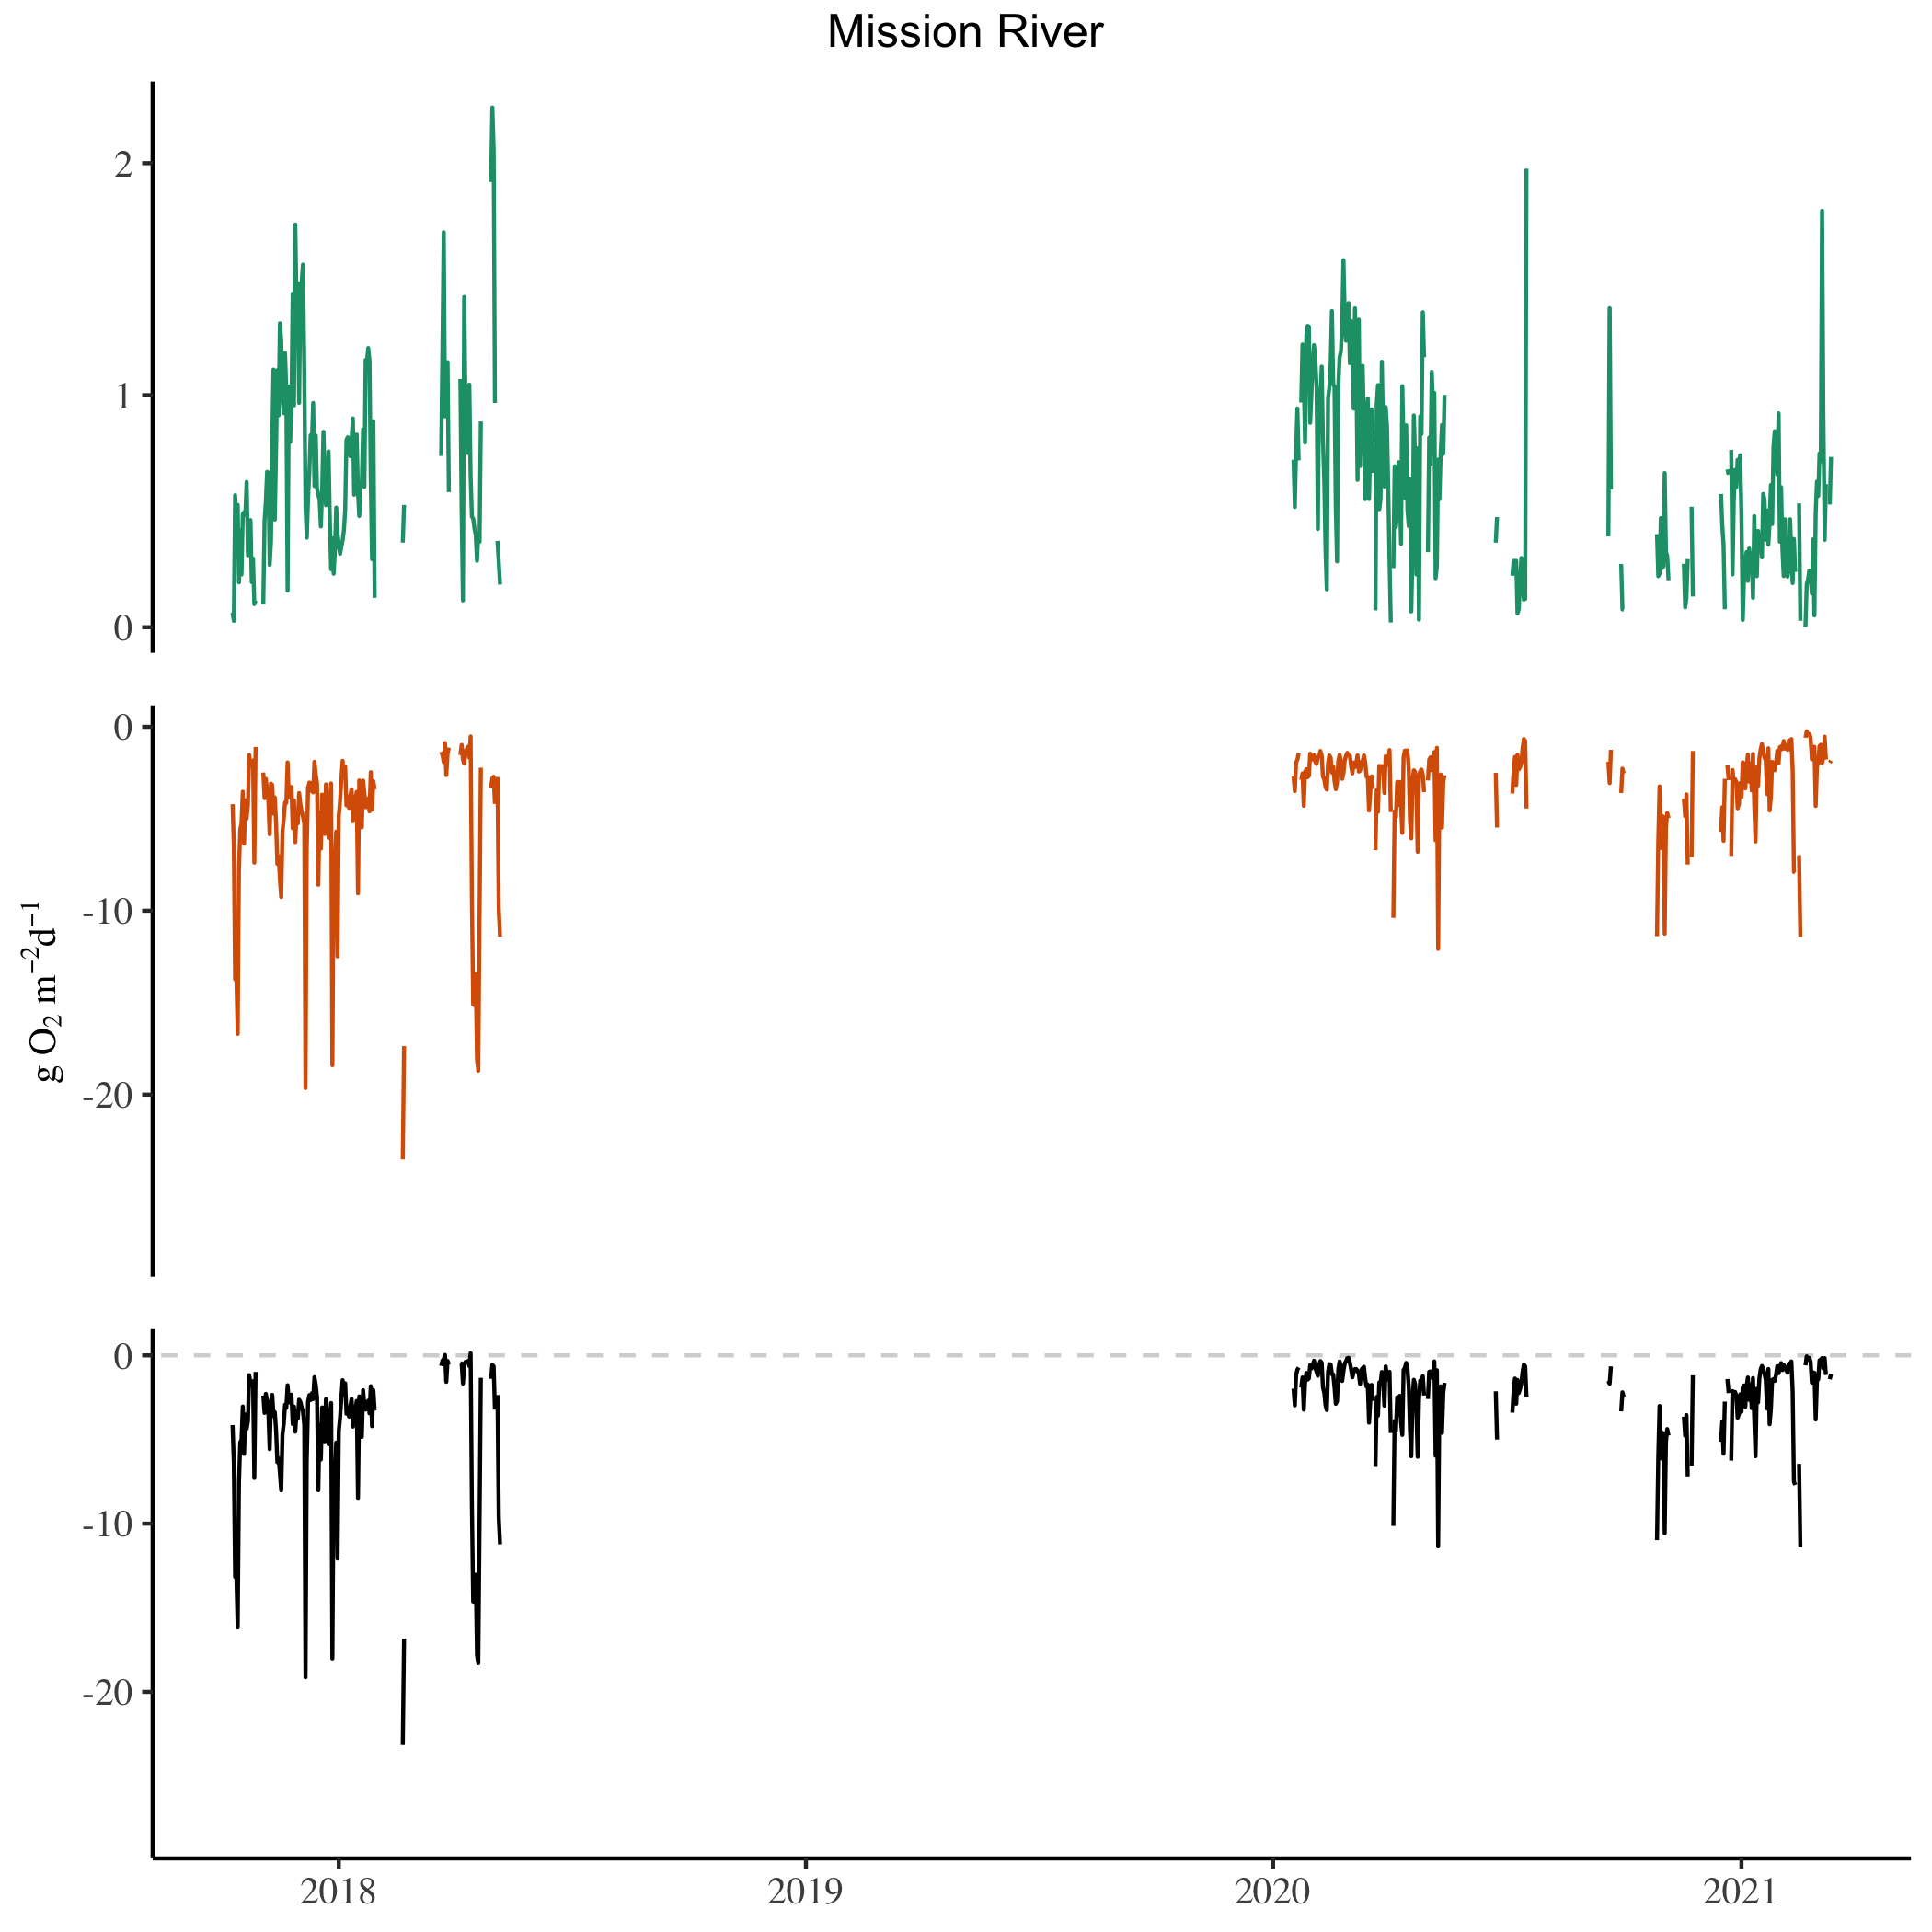
\includegraphics[scale=0.2]{Figs/MR.png}
\caption{Mission River}
\label{Fig:MR}
\end{center}
\end{figure}

\begin{figure}[htb]
\begin{center}
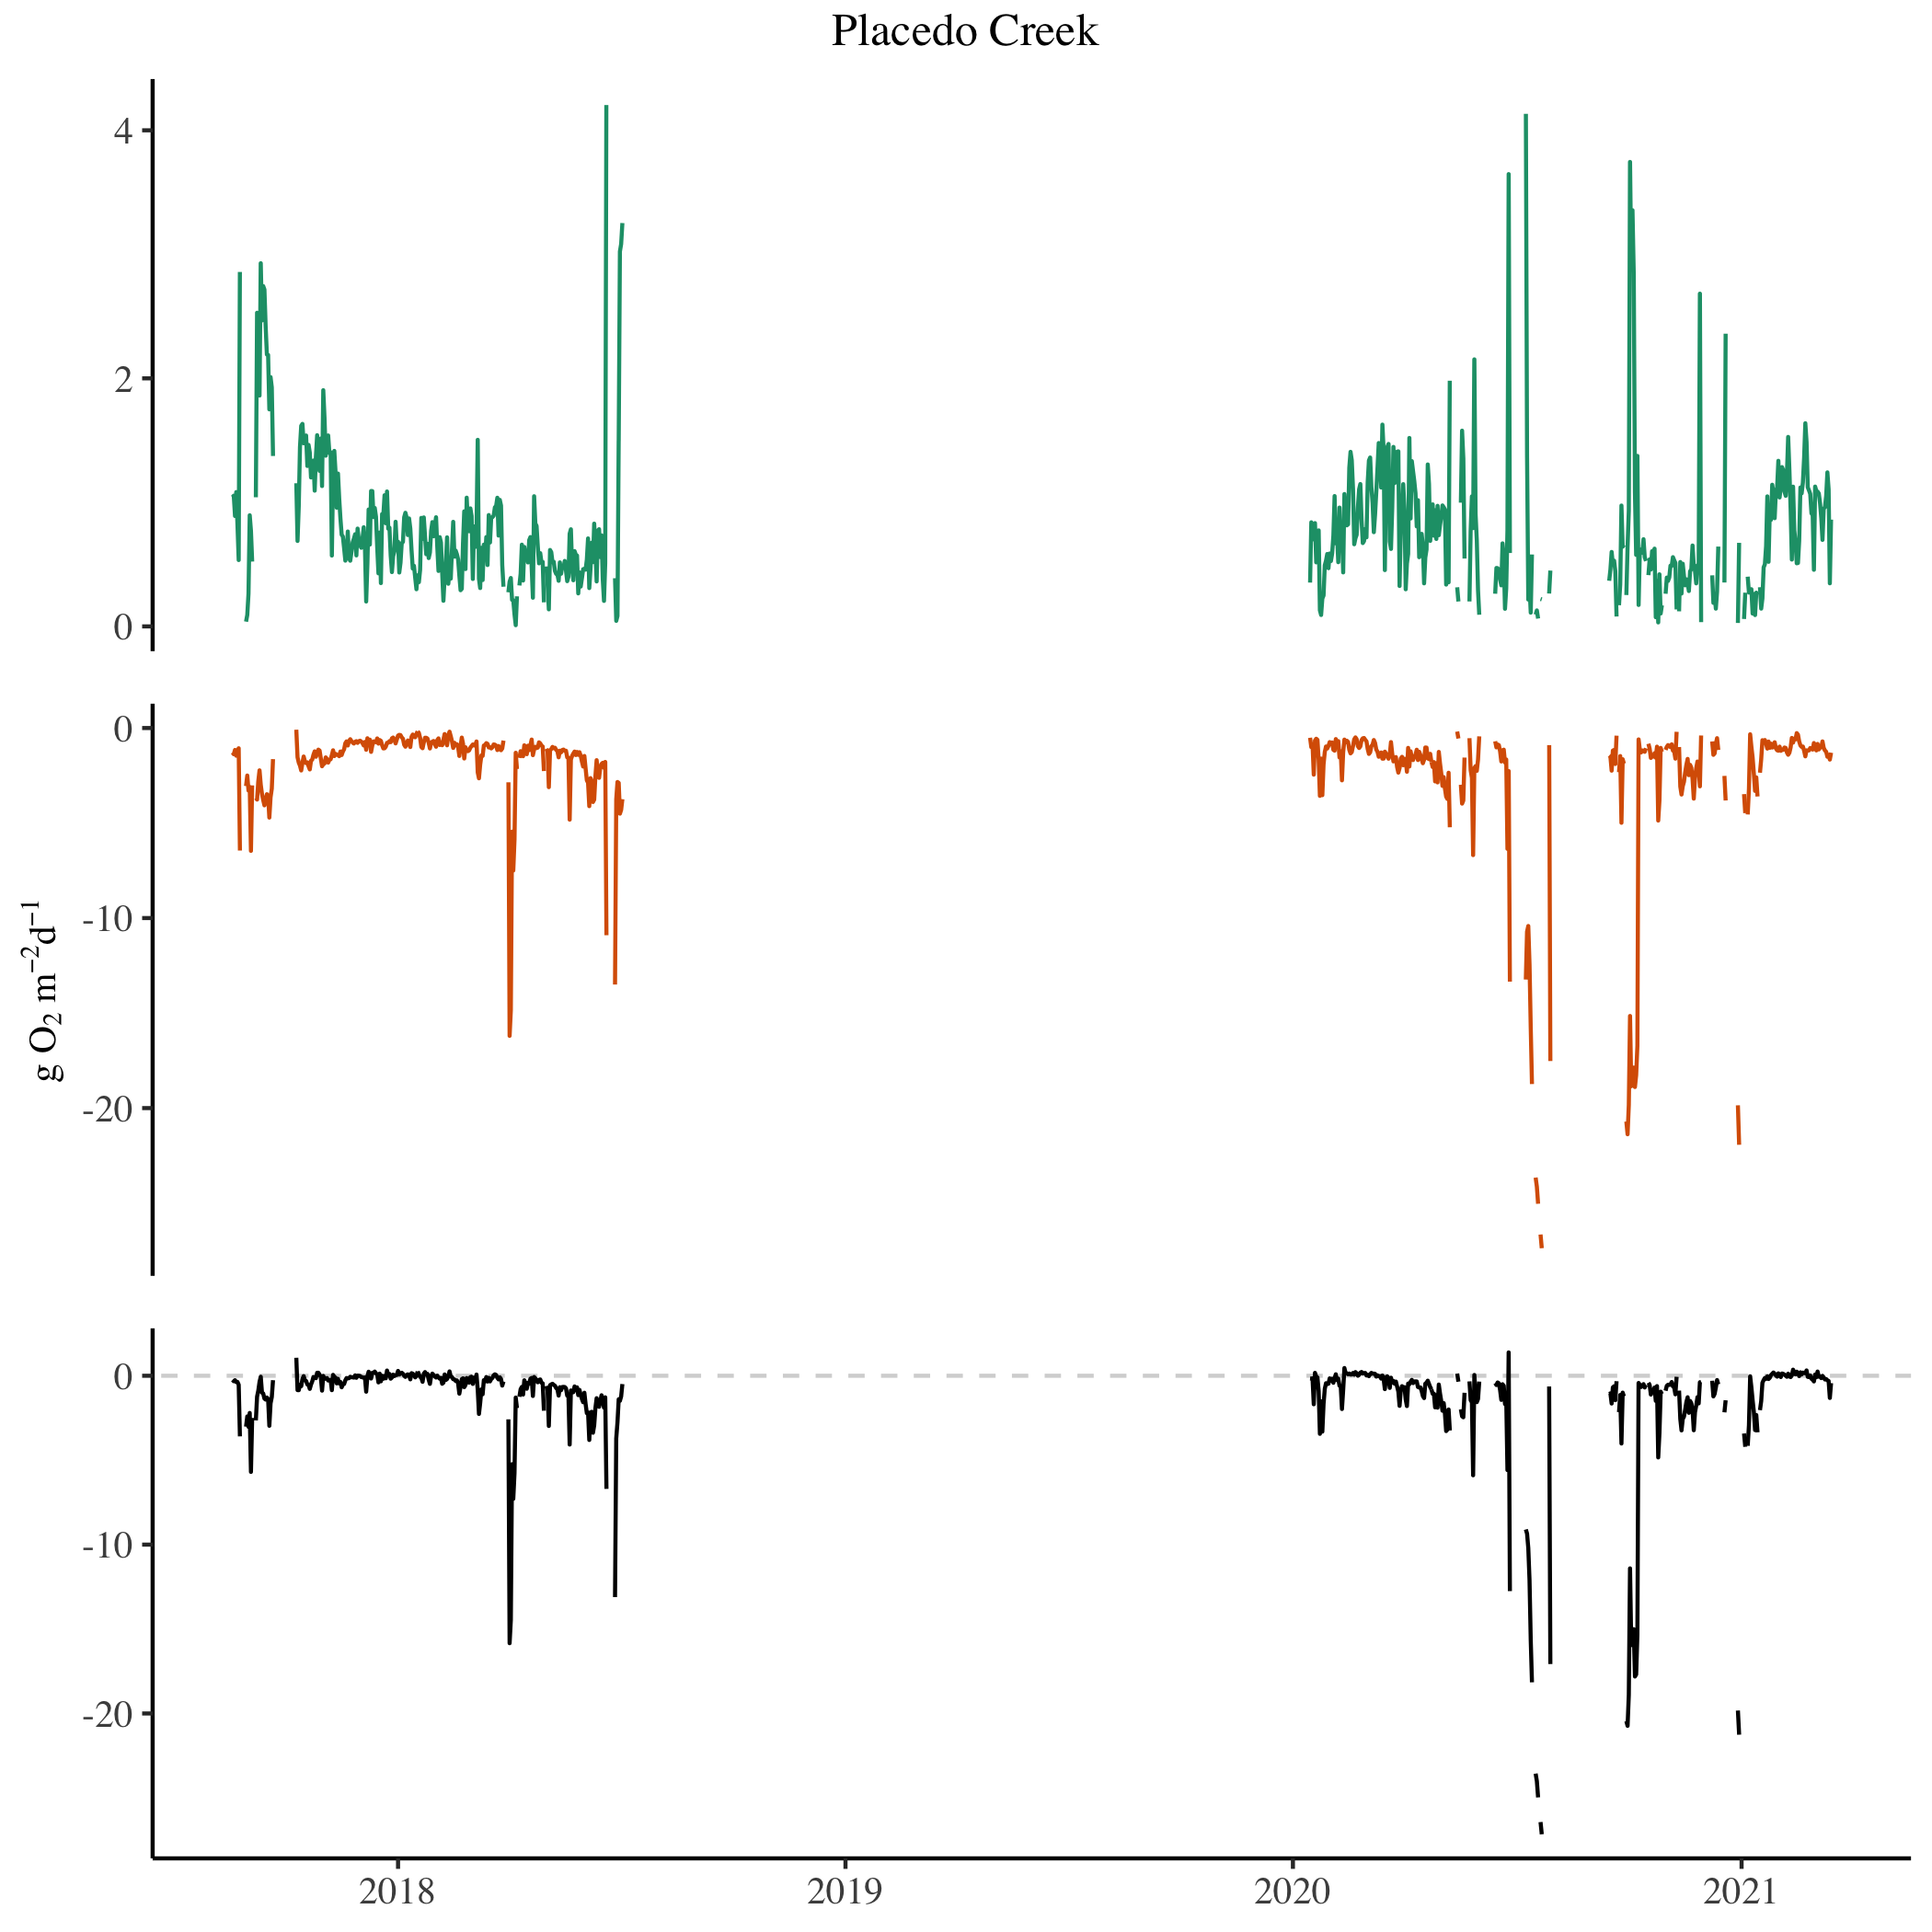
\includegraphics[scale=0.2]{Figs/PLC.png}
\caption{Placedo Creek}
\label{Fig:PLC}
\end{center}
\end{figure}

\begin{figure}[htb]
\begin{center}
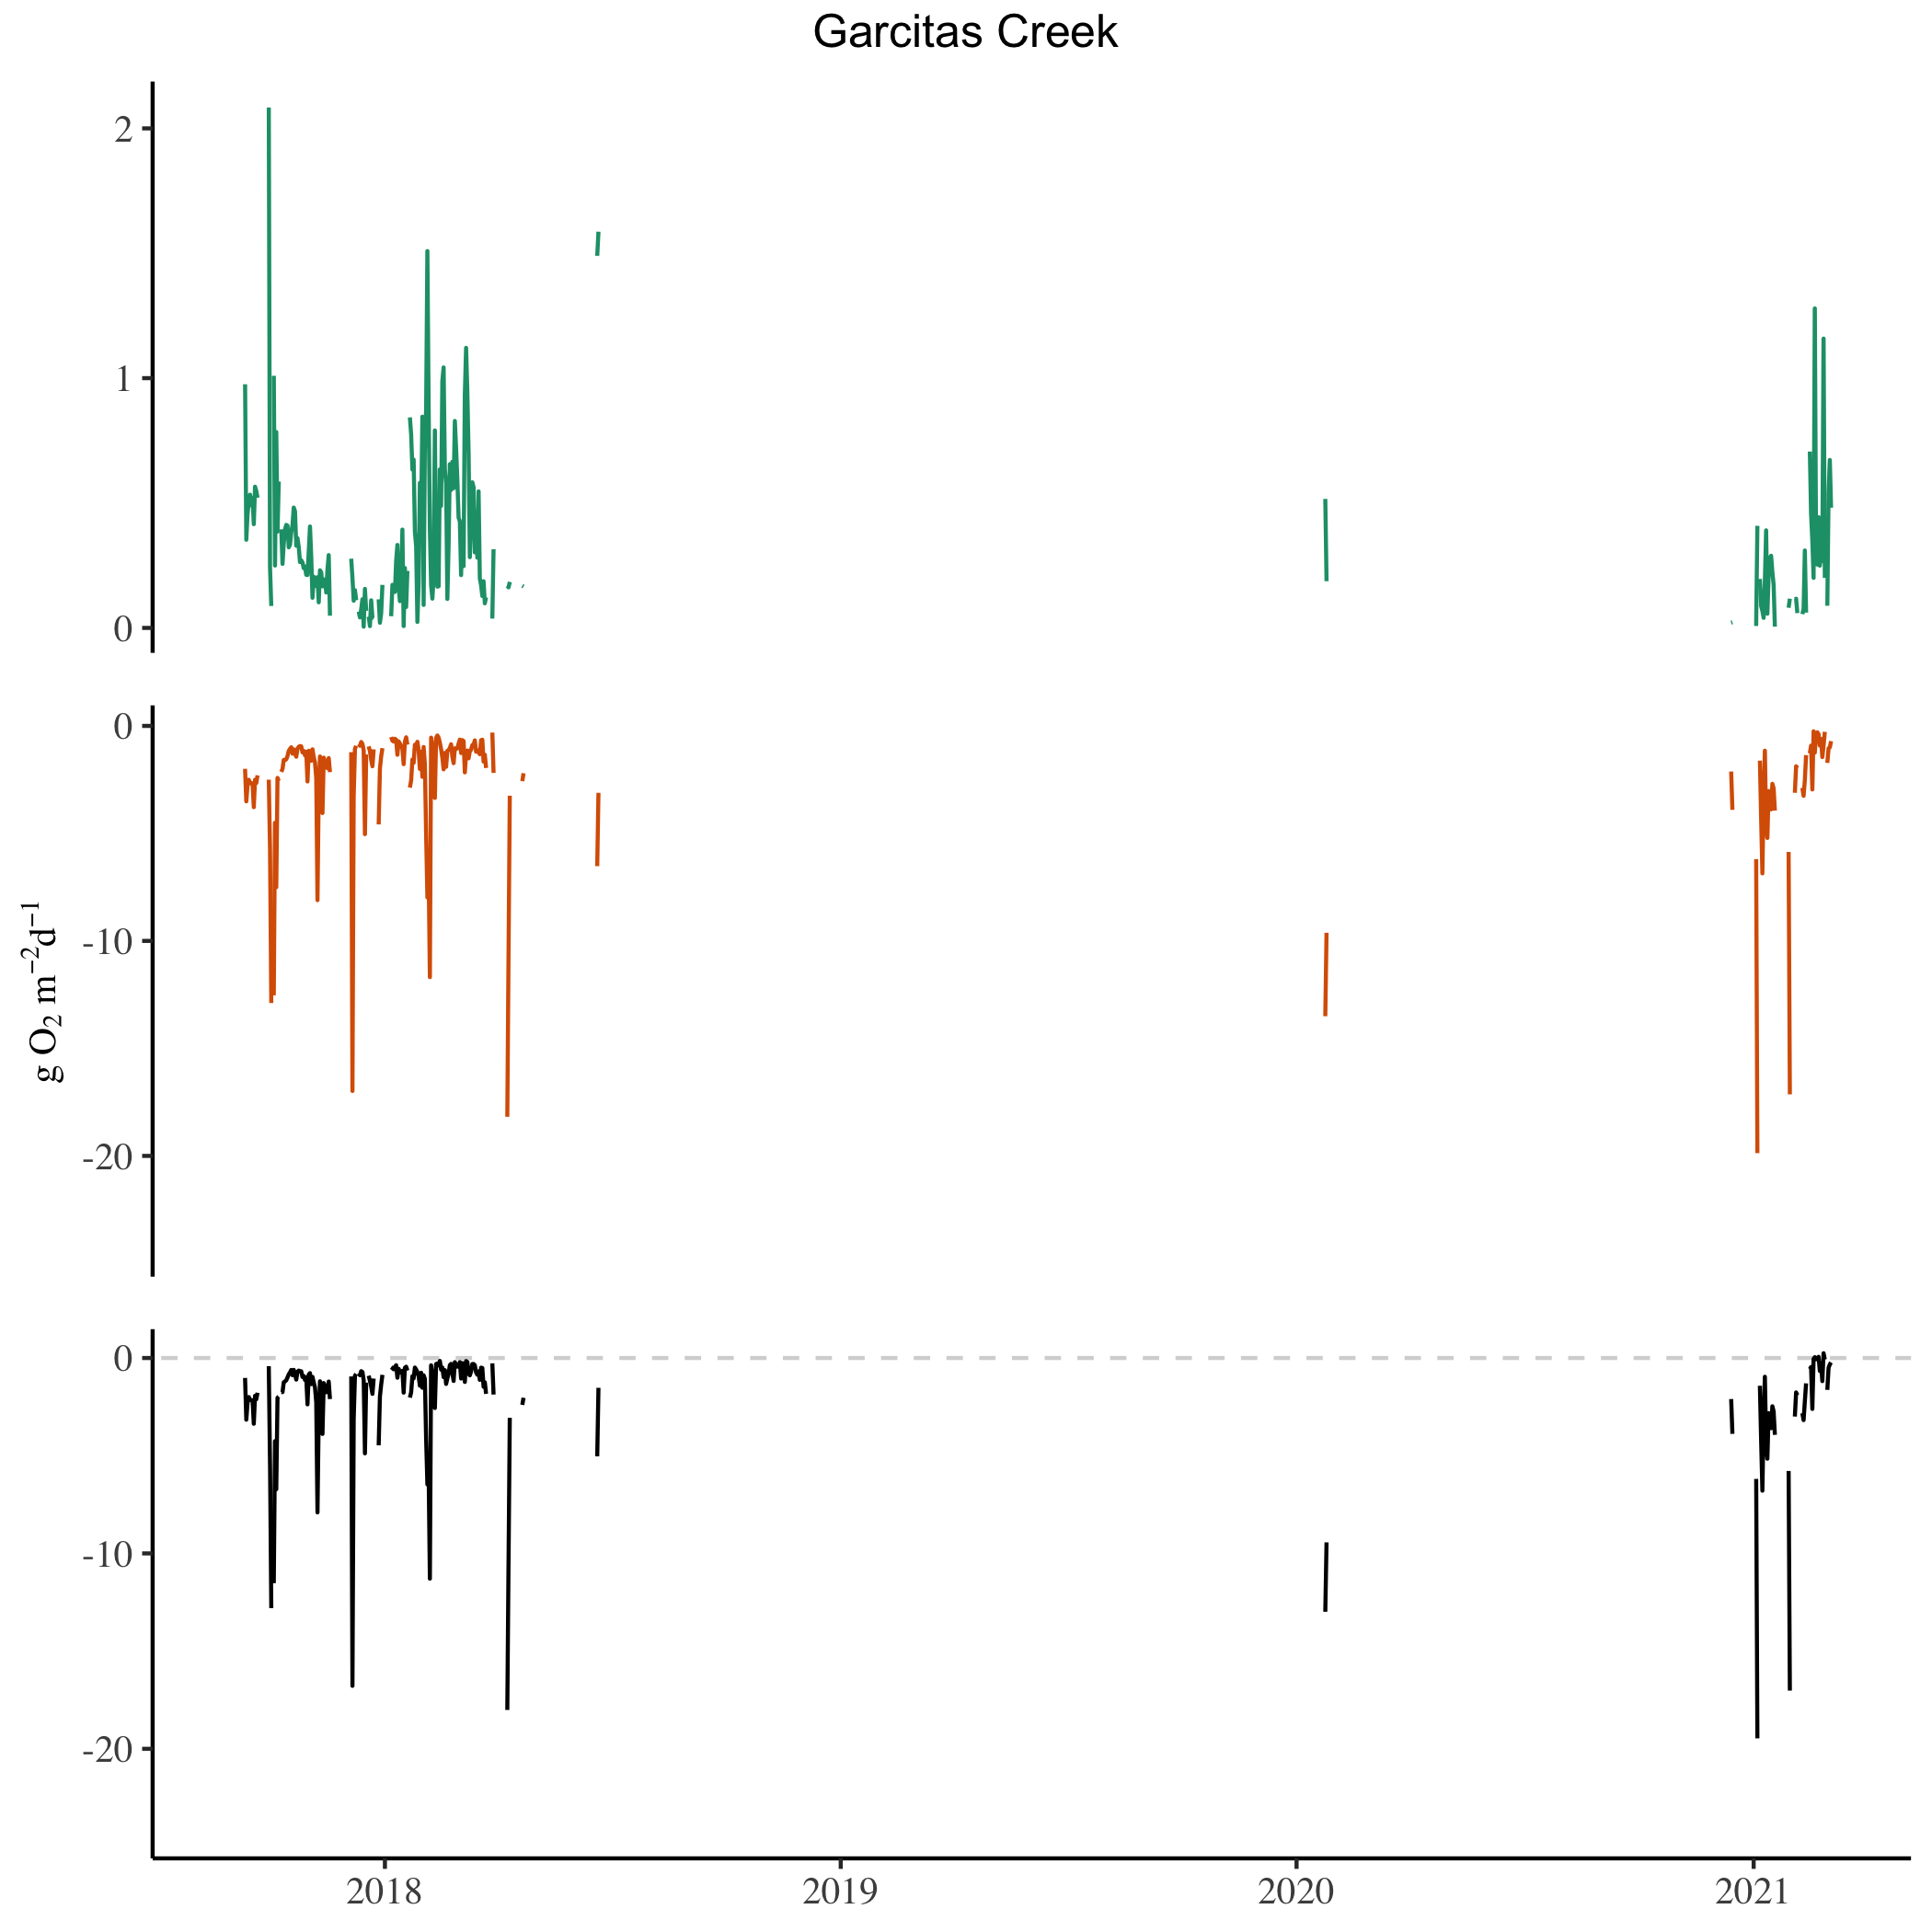
\includegraphics[scale=0.2]{Figs/GC.png}
\caption{Garcitas Creek}
\label{Fig:GC}
\end{center}
\end{figure}

\begin{figure}[htb]
\begin{center}
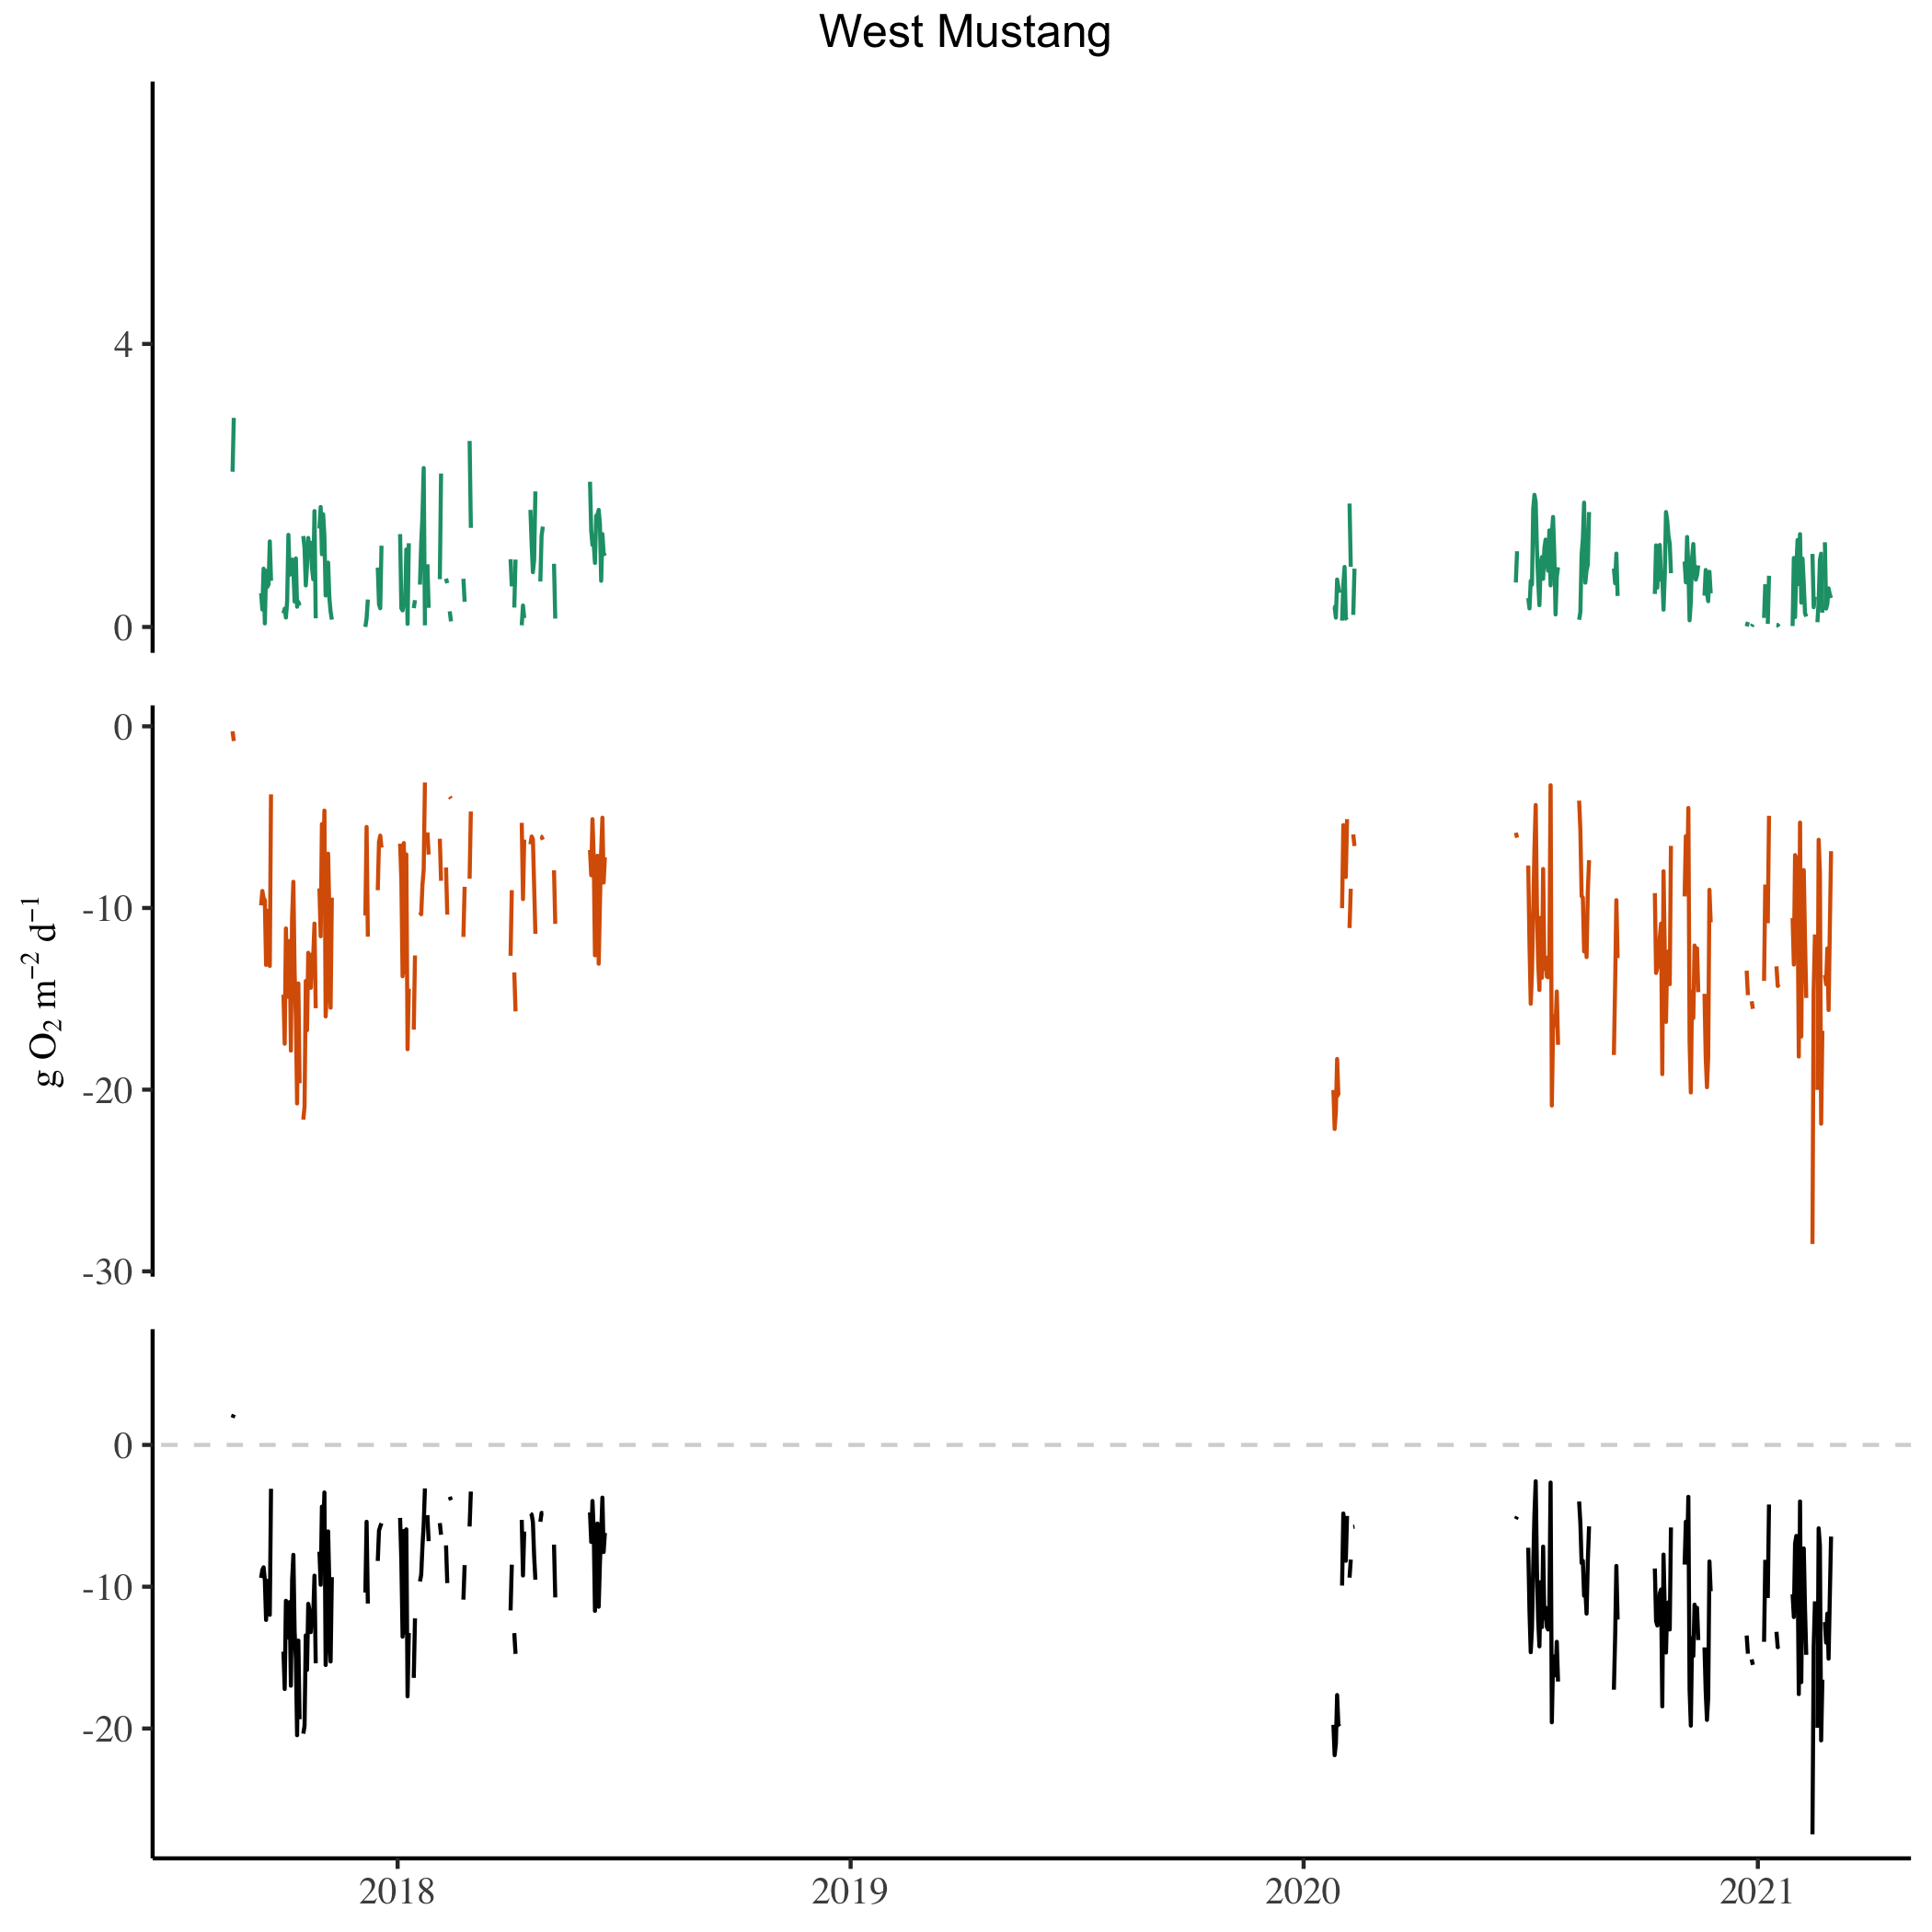
\includegraphics[scale=0.2]{Figs/WMC.png}
\caption{West Mustang Creek}
\label{Fig:WMC}
\end{center}
\end{figure}

\begin{figure}[htb]
\begin{center}
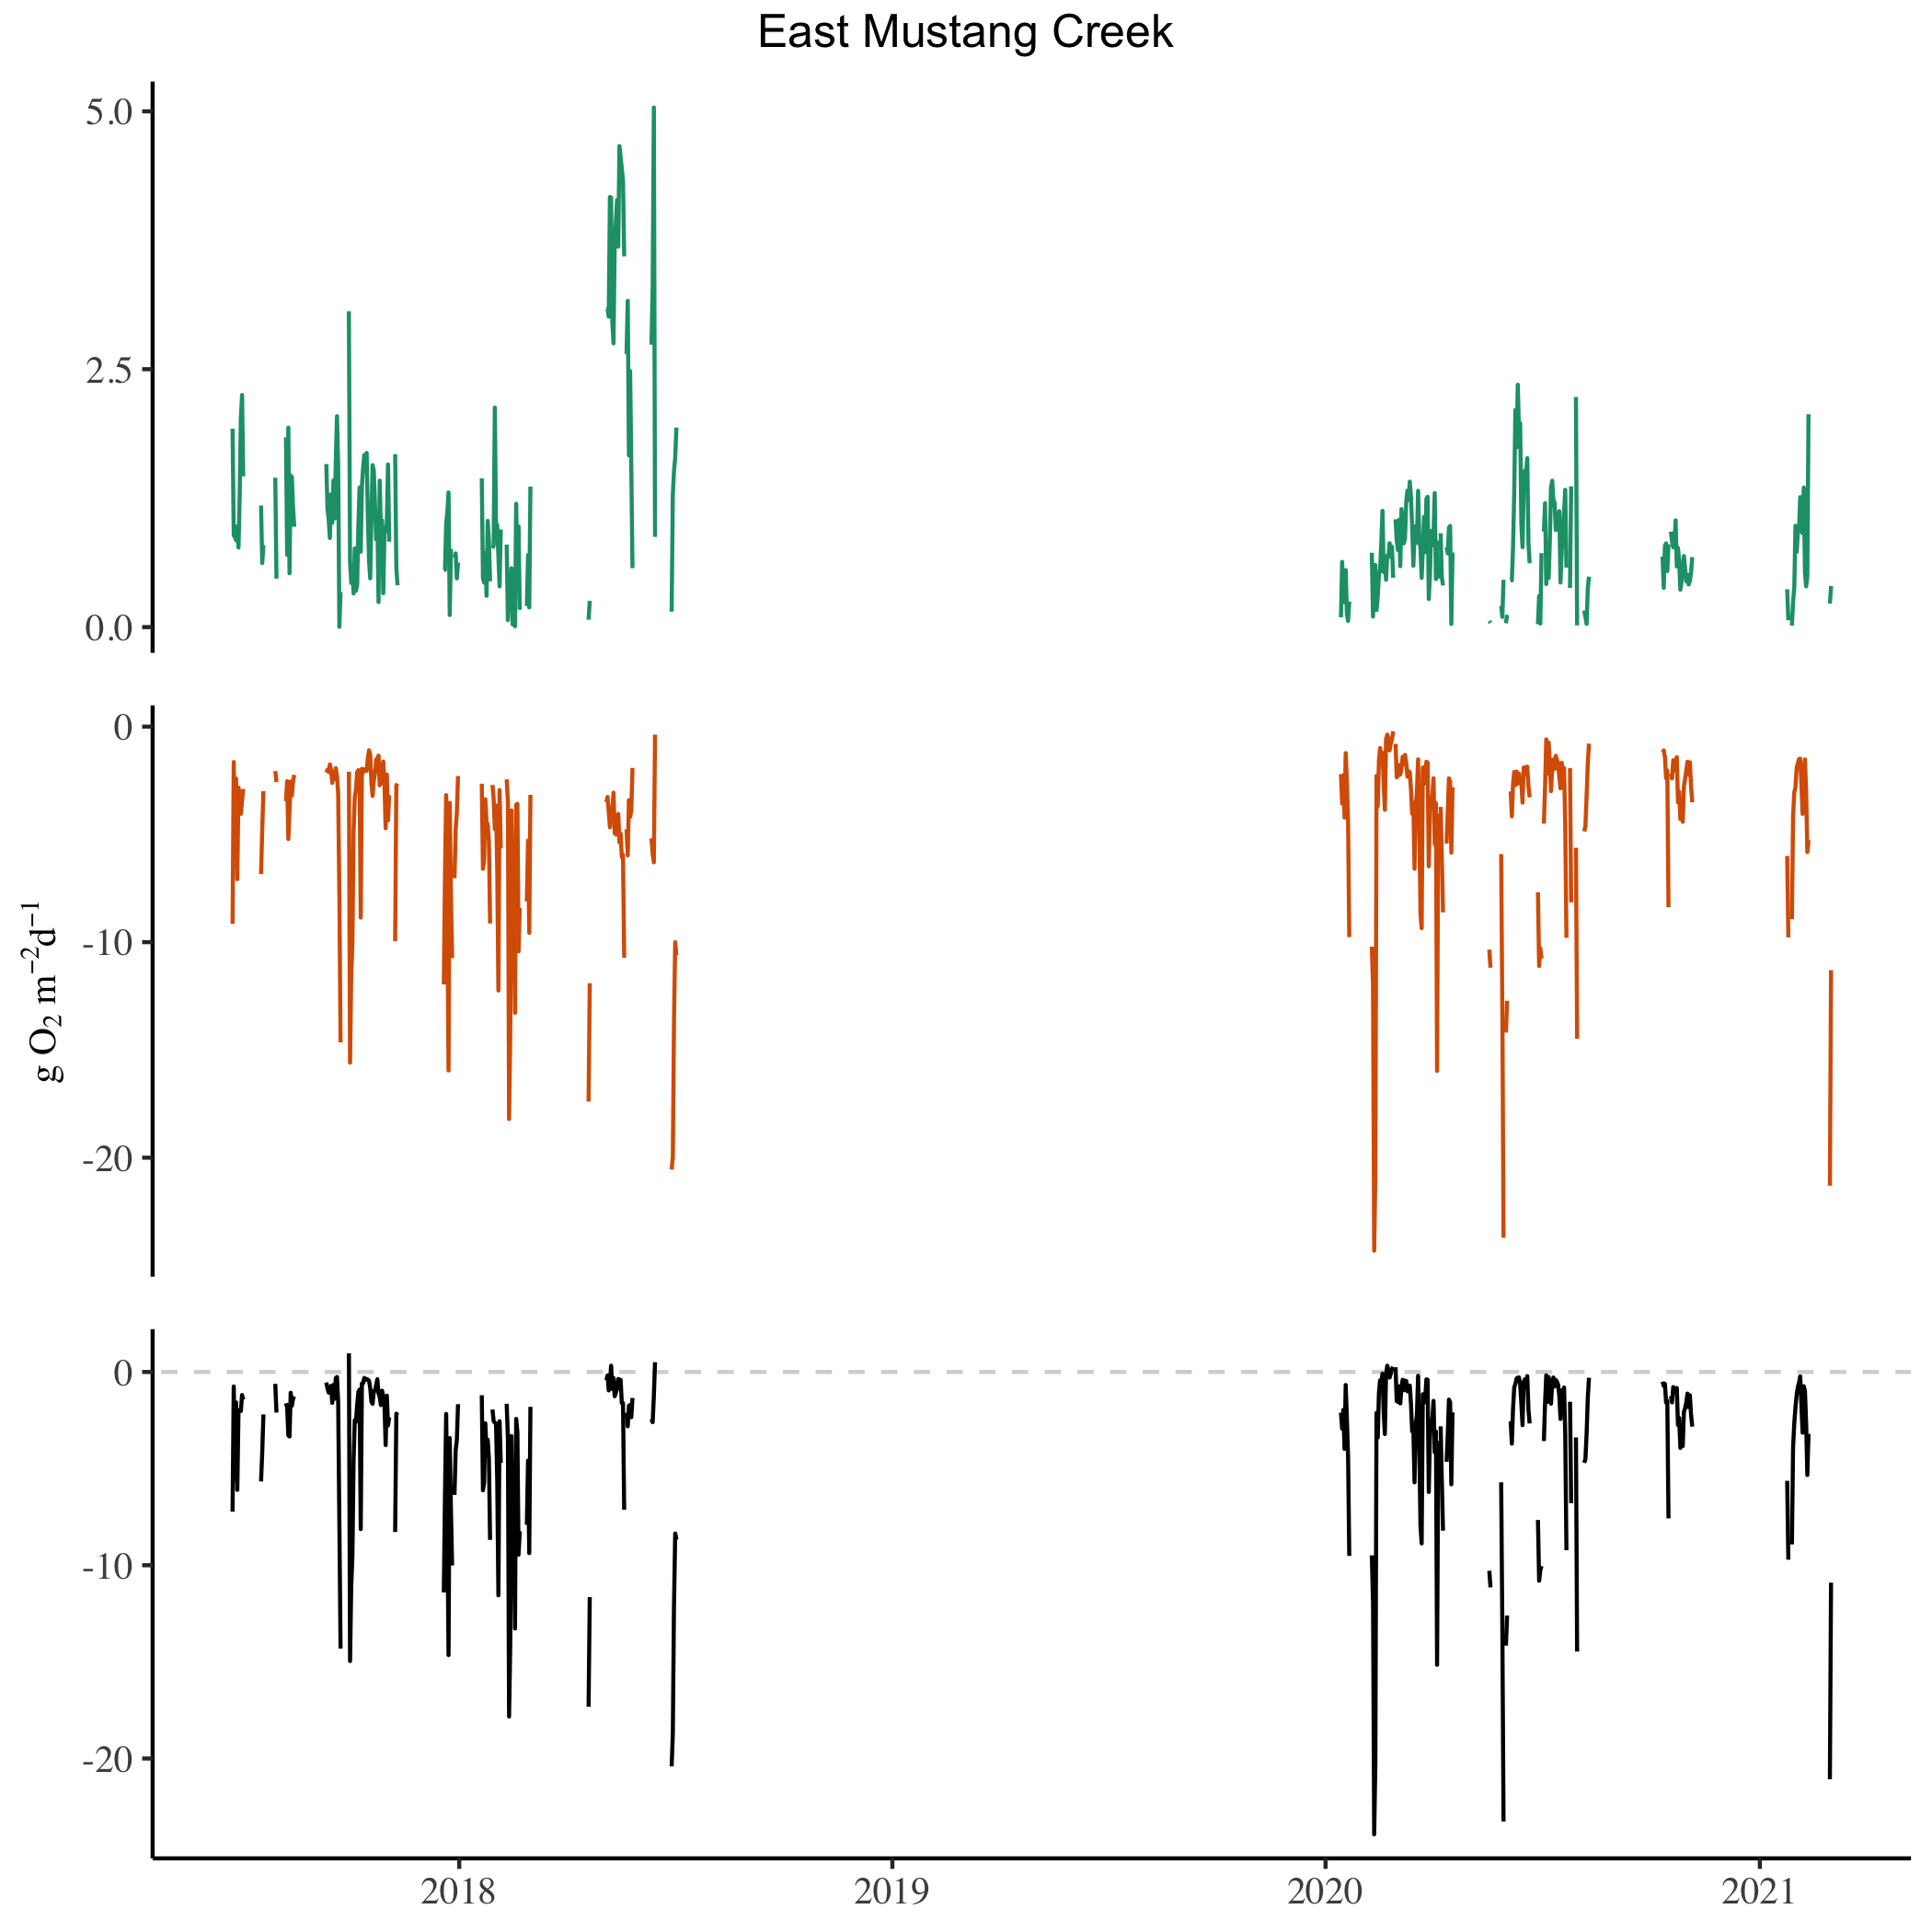
\includegraphics[scale=0.2]{Figs/EMC.png}
\caption{East Mustang Creek}
\label{Fig:EMC}
\end{center}
\end{figure}

\endinput
%-----------------------------------------------------------------------------
% End of appendix1.tex
%-----------------------------------------------------------------------------


%%-----------------------------------------------------------------------------
% Beginning of appendix2.tex
%-----------------------------------------------------------------------------
%
%%%%%%%%%%%%%%%%%%%%%%%%%%%%%%%%%%%%%%%%%%%%%%%%%%%%%%%%%%%%%%%%%%%%%%%%

\chapter{APPENDIX B}
\label{cha:app2}

% Appendices MUST NOT have sections or subsections
%\vspace{-12pt}
%\section{Some Definitions}

\indent \textbf{Anomaly detection.} Detecting anomaly for given statistical models.

\textbf{Classification of objects (Spectral classification).} Classifying
objects in a HSI data set.

\textbf{Demixing.} Finding material components in a raster cell.

\textbf{Electromagnetic radiation (EMR).} The energy in the form of
electromagnetic waves.

\textbf{Electromagnetic spectrum.} The entire family of electromagnetic
radiation, together with all its various wavelengths.

\textbf{Endmember spectra.} The \textquotedblleft pure\textquotedblright%
\ spectra that contribute to mixed spectra.

\textbf{Fused images.} A fused image is a combination of the HSI image and the
HRI image (to be mentioned below). It is usually the best because of high
resolution from the HRI camera and color information from the HSI sensor. This
combination results in sufficiently high image resolution and contrast to
facilitate image evaluation by the human eyes.

\textbf{High Resolution Imagery (HRI).} A high-resolution image (HRI) camera,
which captures black-and-white or panchromatic images, is usually integrated
in an HSI system to capture the same reflected light. However, the HRI camera
does not have a diffraction grating to disperse the incoming reflected light.
Instead, the incoming light is directed to a wider CCD (Charge-Couple Device) to capture more image
data. The HSI resolution is typically one meter per pixel, and the HRI
resolution is much finer: typically a few inches square per pixel.

\textbf{Hyperspectral imaging.} The imagery consists of a larger number of
spectral bands so that the totality of these bands is numerically sufficient
to represent a (continuous) spectral curve for each raster cell.

\textbf{Illumination factors.} The incoming solar energy varies greatly in
wavelengths, peaking in the range of visible light. To convert spectral
radiance to spectral reflectance, the illumination factors must be accounted.
Illumination factors taken into account includes both the illumination
geometry (angles of incoming light, etc.,) and shadowing. Other factors, such
as atmospheric and sensor effects, are also taken into consideration.

\textbf{Macroscopic and intimate mixtures.} Microscopic mixture is a linear
combination of its endmembers, while an intimate mixture is a nonlinear
mixture of its endmembers.

\textbf{Mixed spectra.} Mixed spectra, also known as composite spectra, are
contributed by more than one material components.

\textbf{Multi-spectral imaging.} The imaging bins the spectrum into a handful
of bands.

\textbf{Raster cell.} A pixel in a hyperspectral image.

\textbf{Reflectance conversion.} Radiance values must be converted to
reflectance values before comparing image spectra with reference reflectance
spectra. This is called atmospheric correction. The method for converting the
radiance to reflectance is also called reflectance conversion. The image-based
correction methods include \emph{Flat Field Conversion} and \emph{Internal
Average Relative Reflectance Conversion}. They apply the model $R_{1}=mR_{2},$
where $R_{1}$ is the reflectance, $R_{2}$ is the radiance, and $m$ is the
conversion slope. Some conversions also apply the linear model $R_{1}%
=-c+mR_{2},$ where $c$ is an offset that needs to be abstracted from the
radiance. The popular conversions are

\begin{enumerate}
\item \emph{Flat Field Conversion}. A flat field has a relatively flat
spectral reflectance curve. The mean spectrum of such an area would be
dominated by the combined effects of solar irradiance and atmospheric
scattering and absorption. The scene is converted to "relative" reflectance by
dividing each image spectrum by the flat field mean spectrum.

\item \emph{Internal Average Relative Reflectance (IARR) Conversion}. This
technique is used when no knowledge of the surface materials is available. The
technique calculates a relative reflectance by dividing each spectrum (pixel)
by the scene average spectrum.
\end{enumerate}

\textbf{Region segmentation.} Partitioning the spatial region of a
hyperspectral image into multiple regions (sets of pixels). The goal of
segmentation is to simplify and/or change the representation of an HSI image
into something that is more meaningful and easier to analyze. Region
segmentation is typically used to locate objects and boundaries (lines,
curves, etc.) in images.%

\textbf{Remote sensing.} Sensing something from a distance. The following
processes affect the light that is sensed by a remote sensing system:

% Appendices MUST NOT have sections or subsections
% \section{A Few More Definitions.}

\begin{enumerate}
\item \emph{Illumination}. Light has to illuminate the ground and objects on
the ground before they can reflect any light. In the typical remote sensing
environment, which is outdoors, illumination comes from the sun. We call it
solar illumination.

\item \emph{Atmospheric Absorption and Scattering of Illumination Light}. As
solar illumination travels through the atmosphere, some wavelengths are
absorbed and some are scattered. Scattering is the change in direction of a
light wave that occurs when it strikes a molecule or particle in the atmosphere.

\item \emph{Reflection}. Some of the light that illuminates the ground and
objects on the ground is reflected. The wavelengths that are reflected depend
on the wavelength content of the illumination and on the object's reflectance.
The area surrounding a reflecting object also reflects light, and some of this
light is reflected into the remote sensor.

\item \emph{Atmospheric Absorption and Scattering of Reflected Light}. As
reflected light travels through the atmosphere to the remote sensor, some
wavelengths are absorbed, some are scattered away from the sensor, and some
are scattered into the sensor.
\end{enumerate}

These four effects all change the light that reaches the remote sensor from
the original light source. After the reflected light is captured by the remote
sensor, the light is further affected by how the sensor converts the captured
light into electrical signals. These effects that occur in the sensor are
called sensor effects.

\textbf{Spectral curve.} It is the one-dimensional curve of a spectral reflectance.

\textbf{Spectral libraries.} A spectral library consists of a list of spectral
curves with data of their characteristics corresponding to specific materials
such as mines, plants, etc.

\textbf{Spectral radiance.} It is the measurable reflected light reaching the
sensor. The spectral reflectance of the material is only one factor affecting
it. It is also dependent of the spectra of the input solar energy interactions
of this energy during its downward and upward passages through the atmosphere, etc

\textbf{Shape recognition.} Recognizing the shape of a detected object.

\textbf{Spectral reflectance.} It is the ratio of reflected energy to incident
energy as a function of wavelengths. A certain material has its own spectral
reflectance. The light that is reflected by an object depends on two things:
(1) light that illuminates the object; and (2) the reflectance of the object.
Reflectance is a physical property of the object surface. It is the percentage
of incident EMR of each wavelength that is reflected by the object. Because it
is a physical property, it is not affected by the light that illuminates the object.

\textbf{Spectral reflection.} It is the observed reflected energy, represented
as a function of wavelengths under illumination. It is affected by both
reflectance of the object and the light that illustrates the object. If an
object was illuminated by balanced white light, and if there was no
atmospheric absorption or scatter, and if the sensor was perfect, then the
wavelength composition of reflected light detected by an HSI sensor would
match the reflectance, or spectral signature of the object.

\textbf{Spectral space.} The $n$-dimensional space, where each point is the
spectra of a material or a group of materials.

\textbf{Spectral signature.} A unique characteristic of an object, represented
by some chart of the plot of the object's reflectance as a function of its
wavelength. It can be thought of as an EMR \textquotedblleft
fingerprint\textquotedblright\ of the object.

\textbf{Spectroscopy.} The study of the wavelength composition of
electromagnetic radiation. It is fundamental to how HSI technology works.

\textbf{Signature matching.} Matching reflected light of pixels to spectral
signatures of given objects.

\endinput
%-----------------------------------------------------------------------------
% End of appendix1.tex
%-----------------------------------------------------------------------------



\end{appendices}
%%%%%%%%%%%%%%
%%%%% END  %%%%%%
%%%%%%%%%%%%%%

% \backmatter

%-----------------------------------------------------------------------------
% Beginning of vita.tex
%-----------------------------------------------------------------------------
%
%%%%%%%%%%%%%%%%%%%%%%%%%%%%%%%%%%%%%%%%%%%%%%%%%%%%%%%%%%%%%%%%%%%%%%%%
\clearpage
\phantomsection
\setlength{\parindent}{0pt}
\addcontentsline{toc}{chapter}{VITA}
\begin{singlespace}
\setstretch{1.25}
\begin{center}{\textbf{VITA}}\end{center}
\par
\par
% Put you vita here (below is a sample.)
\begin{center}Connor L. Brown\end{center}

\textbf{EDUCATION}\\
\smallskip\textbf{M.S., Biology} 2019-Present
Sam Houston State University, Huntsville, Texas
Thesis:\\Ecosystem  metabolism  of  coastal  Texas  streams  across  precipitation regimes and land use gradients.\\
\textbf{Relevant Coursework:} Ichthyology, Invertebrate Zoology, Biogeography, Biostatistics, Hydrology, Stream Ecology

\medskip\textbf{B.S., Natural Resources Management} 2016-2018
Texas Tech University, Lubbock, Texas\\
\textbf{Concentration:} Aquatic and Fisheries Biology\\
\textbf{Minor:} Geographic Information Science and Technology\\
\textbf{Relevant Coursework:} Freshwater Bioassessment, Watershed Planning, Fisheries Conservation and Management, Introduction to Geographic Information Systems, Advanced Geographic Information Systems, Cartographic Design, Spatial Analysis, GPS Mapping, Aerial Photo Interpretation, Integrated Natural Resources Management Skills, Wildlife and Vegetation Techniques, Diversity of Life, Genetics, Introduction to Conservation Science.

\bigskip\textbf{PUBLICATIONS}

\smallskip\textbf{Brown, C. L.} Delaune, K. D., Pease, A. A. 2022. \textit{Benthic Macroinvertebrate Assemblage Structure in Salinized Reaches of the Lower Pecos River, Texas.} (In Review.). The Southwestern Naturalist
\bigskip

\textbf{EXPERIENCE}

\smallskip\textbf{2020-2021} Graduate Research Assistant\\Stream and Biogeochemistry Lab, Department of Biological Sciences, Sam Houston State University.\\Managed data collection, analyzed time series data, estimated ecosystem metabolism using R, and collected macroinvertebrates and fish for the NSF Funded project Thresholds in Ecosystem Responses to Rainfall Gradients (TERRG).

\medskip\textbf{2019} Graduate Research Assistant\\Texas Research Institute for Environmental Studies, Sam Houston State University\\Worked on a funded grant from the Texas Military Department to collect invertebrate and habitat data, identified terrestrial and aquatic invertebrates, and pinned specimens.

\medskip\textbf{2019-2020} Teaching Assistant\\Department of Biological Sciences, Sam Houston State University\\Taught three sections of Ecology Lab and Environmental Science. This included giving a lecture over the material, leading lab activities, and assisting in students' knowledge of ecology and environmental science.

\medskip\textbf{2016-2018} Undergraduate Researcher\\Department of Natural Resources Management, Texas Tech University\\Proposed and conducted a research project on the Pecos River. Field work included setting up Hester-Dendy samplers at three sites along the Pecos and taking habitat measurements. Lab work included sorting macroinvertebrates and identifying them using dichotomous keys.

\medskip\textbf{2016} Undergraduate Internship\\Department of Natural Resources Management, Texas Tech University\\Worked closely with a graduate student on their dissertation with both field and lab work. Field work included setting up transects, collecting macroinvertebrates, fish, water sampling, as well as taking habitat measurements. Lab work included using dichotomous keys to identify macroinvertebrates as well as extracting environmental DNA from water samples.

\bigskip\textbf{PRESENTATIONS}

\smallskip\textbf{Brown, C. L.}, Carvallo, F., Frazier, C., Groff, C.M., Jenkins, V., Kinard, S. K., Solis, A.T., Strickland, B., Hogan, J. D., Patrick, C. J., Whiles, M. R., Zanden, H. V., Ulseth, A. J., 2021. Ecosystem metabolism of coastal Texas streams across precipitation and land use gradients. Society for Freshwater Science.

\medskip\textbf{Brown, C. L.}, Delaune, K. D., Pease, A. A., 2018. Spatial and Temporal Variation in Benthic Macroinvertebrate Assemblages Structure in Salinized Reaches of the Pecos River. Desert Fishes Council, Death Valley, California.

\medskip\textbf{Brown, C. L.}, Delaune, K. D., Pease, A. A., 2018. Macroinvertebrate community structure on the lower Pecos River. Southwestern Association of Naturalists, San Marcos, Texas.
\end{singlespace}
\endinput
%-----------------------------------------------------------------------------
% End of vita.tex
%-----------------------------------------------------------------------------



\end{document}  % The End
